% Author Alfredo Sánchez Alberca (asalber@ceu.es)
%!TEX program = pdflatex
\documentclass[a4paper,titlepage]{article}
%===============================================
\usepackage[english]{babel}
\usepackage[utf8]{inputenc}
\usepackage[top=3cm, bottom=3cm, left=2.54cm, right=2.54cm, marginparwidth=2mm]{geometry}

% COLORS
\usepackage[table]{xcolor}
\definecolor{color1}{RGB}{5,161,230} % Light blue
\definecolor{color2}{RGB}{238,50,36} % Red
\definecolor{color3}{RGB}{0,205,0} % Light Green
\definecolor{ocre}{RGB}{243,102,25} % Define the orange color used for highlighting throughout the book
\definecolor{blueceu}{RGB}{5,161,230} % Blue color of CEU logo
\definecolor{greenceu}{RGB}{185,209,16} % Green color of CEU logo
\definecolor{redceu}{RGB}{238,50,36} % Red color of CEU logo
\definecolor{grayceu}{RGB}{111,107,83} % Gray color of CEU logo
\definecolor{chaptergrey}{RGB}{5,161,230} % Blue color of CEU logo

% MATH
\usepackage{amsmath}
\usepackage{amssymb}
\usepackage{amsthm}
\DeclareMathOperator{\sen}{sen}
\DeclareMathOperator{\arcsen}{arcsen}
\DeclareMathOperator{\tg}{tg}
\DeclareMathOperator{\arctg}{arctg}

% GRAPHICS
\usepackage{graphicx}
\usepackage{tikz}
\usepackage{pgfplots}

\usepackage{multicol}
\usepackage[inline]{enumitem}
\usepackage{fancyhdr}
\pagestyle{fancy}
\lhead{\textsc{\textcolor{blueceu}{CEU San Pablo University}}}
\rhead{\textsl{\textsf{\textcolor{blueceu}{Department of Applied Math and Statistics}}}}
\renewcommand{\headrulewidth}{0pt}

\usepackage{booktabs}


% SECTIONS
\usepackage{titlesec}
\titleformat*{\section}{\normalfont\Large\bfseries\color{color1}}


% % SOLUTIONS
% \newif\ifsolution
% % \solutiontrue  % Comment to hide solutions
%
% \newtheoremstyle{solution} % Theorem style name
% {-5pt} % Space above
% {7pt} % Space below
% {\normalfont} % Body font
% {-28pt} % Indent amount
% {\bf} % Theorem head font
% {\kern-11.5pt} % Punctuation after theorem head
% {19pt} % Space after theorem head
% {\begin{tikzpicture}
% \draw (0,0) node [fill=color2, xshift=4mm, inner
% sep=2pt]{
\includegraphics[scale=0.3]{img/bulb}};
% \end{tikzpicture}}
%
% \theoremstyle{solution}
% \newtheorem{solutionT}{Solution}
%
% \RequirePackage[framemethod=default]{mdframed}
%
% % Solution box
% \newmdenv[skipabove=7pt,
% skipbelow=10pt,
% rightline=false,
% leftline=true,
% topline=false,
% bottomline=false,
% linecolor=color2,
% backgroundcolor=black!5,
% innerleftmargin=5pt,
% innerrightmargin=5pt,
% innertopmargin=4pt,
% innerbottommargin=5pt,
% leftmargin=0pt,
% rightmargin=0pt,
% linewidth=4pt]{solBox}
%
% \usepackage{comment}
% \ifsolution
%   \newenvironment{sol}{\ifsolution\begin{solBox}\begin{solutionT}}{\end{solutionT}\end{solBox}\fi}
% \else
%   \excludecomment{sol}
% \fi

% PDF
\usepackage[colorlinks=true]{hyperref}
\hypersetup{pdfauthor={Alfredo Sánchez Alberca (asalber@ceu.es)}, pdftitle={Statistics problems} }
\usepackage{url}

\renewcommand{\floatpagefraction}{.8}
\renewcommand{\textfraction}{.1}

% SOLUTIONS SETTINGS
\usepackage{probsoln-alf}
\reversemarginpar
\showshortanswers
%\showanswers
%\PSNrandseed{2007}

\begin{document}
\sloppy

\title{\vskip 2cm
\Huge \textbf{\textsf{\quad \textcolor{blueceu}{STATISTICS PROBLEMS}\quad}}\\
\vskip 1cm
\Large \sffamily
\begin{tabular}{rl}
\textcolor{blueceu}{Subject:} & Statistics Applied to Health Sciences            \\
\textcolor{blueceu}{Course:}  & 2\textsuperscript{nd}                            \\
\textcolor{blueceu}{Degree:}  & Physiotherapy                                    \\
\textcolor{blueceu}{Year:}    & 2020-2021                                        \\
\textcolor{blueceu}{Authors:}
                              & Alfredo S\'anchez Alberca (\url{asalber@ceu.es})
\end{tabular}
}

\author{}
\date{
\includegraphics[scale=0.3]{img/logo_uspceu}}

\maketitle
\newpage
\tableofcontents
\newpage

% Author Alfredo Sánchez Alberca (asalber@ceu.es)

\newproblem*{des-1a}{far}{}
%STATEMENT
{A survey about the daily number of medicines consumed by people over 70 years, shows the following results:

\begin{center}
3\quad 1\quad 2\quad 2\quad 0\quad 1\quad 4\quad 2\quad 3\quad 5\quad 1\quad 3\quad 2\quad 3\quad 1\quad 4\quad 2\quad 4\quad 3\quad 2 \\
3\quad 5\quad 0\quad 1\quad 2\quad 0\quad 2\quad 3\quad 0\quad 1\quad 1\quad 5\quad 3\quad 4\quad 2\quad 3\quad 0\quad 1\quad 2\quad 3
\end{center}

\begin{enumerate}
\item Construct the frequency distribution table of the sample.
\item Draw the bar chart of the sample and the polygon.
\item Draw the cumulative relative frequency bar chart and polygon.
\end{enumerate}
}
%SOLUTION
{
}
%RESOLUTION
{}

\newproblem{des-1b}{far}{}
%STATEMENT
{Se realizó una encuesta a 40 personas de más de 70 años sobre el número de medicamentos distintos que tomaban habitualmente. El resultado de dicha encuesta fue el siguiente:
\begin{center}
3\quad 1\quad 2\quad 2\quad 0\quad 1\quad 4\quad 2\quad 3\quad 5\quad 1\quad 3\quad 2\quad 3\quad 1\quad 4\quad 2\quad 4\quad 3\quad 2 \\
3\quad 5\quad 0\quad 1\quad 2\quad 0\quad 2\quad 3\quad 0\quad 1\quad 1\quad 5\quad 3\quad 4\quad 2\quad 3\quad 0\quad 1\quad 2\quad 3
\end{center}
Calcular los siguientes estadísticos:
\begin{enumerate}
\item Media.
\item Mediana.
\item Moda.
\item Varianza.
\item Desviación típica.
\item Coeficiente de variación.
\end{enumerate}
}
%SOLUTION
{\begin{enumerate}
\item $ \bar{x} = 2.225$ medicamentos.
\item $Med =2$ medicamentos.
\item $Mod= 2$ y $3$ medicamentos.
\item $s^2 = 1.974$ medicamentos$^2$.
\item $s= 1.405$ medicamentos.
\item $cv = 0.632$, lo que indica que la hay una dispersión moderada-alta.
\end{enumerate}
}
%RESOLUTION
{}


\newproblem*{des-2a}{far}{}
%STATEMENT
{The number of people treated in the emergency service of a hospital every day of November
was
\begin{center}
15 \quad 23 \quad 12 \quad 10 \quad 28 \quad 7 \quad 12 \quad 17 \quad 20 \quad 21 \quad 18 \quad 13 \quad 11 \quad 12 \quad 26 \\
30 \quad 6 \quad 16 \quad 19 \quad 22 \quad 14 \quad 17 \quad 21 \quad 28 \quad 9 \quad 16 \quad 13 \quad 11 \quad 16 \quad 20
\end{center}

\begin{enumerate}
\item Construct the frequency distribution table of the sample.
\item Draw a suitable chart for the frequency distribution.
\item Draw a suitable chart for the cumulative frequency distribution.
\end{enumerate}
}
%SOLUTION
{
}
%RESOLUTION
{}


\newproblem{des-2b}{far}{}
%STATEMENT
{En un hospital se realizó un estudio sobre el número de personas que ingresaron en urgencias en el mes de noviembre. Los datos observados fueron:
\begin{center}
115 \quad 23 \quad 12 \quad 10 \quad 28 \quad 7 \quad 12 \quad 17 \quad 20 \quad 21 \quad 18 \quad 13 \quad 11 \quad 12 \quad 26 \\
30 \quad 6 \quad 16 \quad 19 \quad 22 \quad 14 \quad 17 \quad 21 \quad 28 \quad 9 \quad 16 \quad 13 \quad 11 \quad 16 \quad 20
\end{center}
Calcular los siguientes estadísticos:
\begin{enumerate}
\item Media aritmética
\item Mediana.
\item Moda.
\item Tercer decil.
\item Percentil 62.
\end{enumerate}
}
%SOLUTION
{
Agrupando en las clases $(5,10]$, $(10,15]$, $(15,20]$, $(20,25]$, $(25,30]$.
\begin{enumerate}
\item $\bar{x} = 16.67$ ingresos.
\item $Me=16.11$ ingresos.
\item $Mo=(10,15]$ y $(15,20]$ ingresos.
\item $D_3=12.78$ ingresos.
\item $P_{62}=18.1$ ingresos.
\end{enumerate}
}
%RESOLUTION
{}


\newproblem{des-2c}{far}{}
%STATEMENT
{En un hospital se realizó un estudio sobre el número de personas que ingresaron en urgencias en el mes de noviembre. Los datos observados fueron:
\begin{center}
115 \quad 23 \quad 12 \quad 10 \quad 28 \quad 7 \quad 12 \quad 17 \quad 20 \quad 21 \quad 18 \quad 13 \quad 11 \quad 12 \quad 26 \\
30 \quad 6 \quad 16 \quad 19 \quad 22 \quad 14 \quad 17 \quad 21 \quad 28 \quad 9 \quad 16 \quad 13 \quad 11 \quad 16 \quad 20
\end{center}
Calcular los siguientes estadísticos:
\begin{enumerate}
\item Varianza
\item Desviación típica.
\item Coeficiente de variación de Pearson.
\end{enumerate}
}
%SOLUTION
{
Agrupando en las clases $(5,10]$, $(10,15]$, $(15,20]$, $(20,25]$, $(25,30]$.
\begin{enumerate}
\item $s^2 = 36.75$ ingresos$^2$.
\item $s=6.06$ ingresos.
\item $cv=0.365$, lo que indica que hay poca dispersión.
\end{enumerate}
}
%RESOLUTION
{}


\newproblem*{des-3a}{fis}{*}
%STATEMENT
{The number of injuries suffered by the members of a soccer team in a league were
\begin{center}
0 \quad 1 \quad 2 \quad 1 \quad 3 \quad 0 \quad 1 \quad 0 \quad 1 \quad 2 \quad 0 \quad 1 \\
1 \quad 1 \quad 2 \quad 0 \quad 1 \quad 3 \quad 2 \quad 1 \quad 2 \quad 1 \quad 0 \quad 1
\end{center}

Compute:
\begin{enumerate}
\item Construct the frequency distribution table of the sample.
\item Draw the bar chart of the sample and the polygon.
\item Draw the cumulative frequency bar chart and polygon.
\end{enumerate}
}
%SOLUTION
{
}
%RESOLUTION
{}


\newproblem{des-3b}{fis}{*}
%STATEMENT
{The number of injuries suffered by the members of a soccer team in a league were
\begin{center}
0 \quad 1 \quad 2 \quad 1 \quad 3 \quad 0 \quad 1 \quad 0 \quad 1 \quad 2 \quad 0 \quad 1 \\
1 \quad 1 \quad 2 \quad 0 \quad 1 \quad 3 \quad 2 \quad 1 \quad 2 \quad 1 \quad 0 \quad 1
\end{center}
\begin{enumerate}
\item Mean.
\item Median.
\item Mode.
\item Quartiles.
\item Percentile 32.
\end{enumerate}
}
%SOLUTION
{\begin{enumerate}
\item $\bar{x}= 1.125$ injuries.
\item $Me=1$ injuries.
\item $Mo=1$ injuries.
\item $C_1 = 0.5$ injuries, $C_2=1$ injuries y $C_3=2$ injuries.
\item $P_{32}=1$ injury.
\end{enumerate}
}
%RESOLUTION
{}


\newproblem{des-3c}{fis}{*}
%STATEMENT
{El número de lesiones padecidas durante una temporada por cada jugador de un equipo de fútbol fue el siguiente:
\begin{center}
0 \quad 1 \quad 2 \quad 1 \quad 3 \quad 0 \quad 1 \quad 0 \quad 1 \quad 2 \quad 0 \quad 1 \\
1 \quad 1 \quad 2 \quad 0 \quad 1 \quad 3 \quad 2 \quad 1 \quad 2 \quad 1 \quad 0 \quad 1
\end{center}
Se pide:
\begin{enumerate}
\item rango intercuartílico e interpretarlo.
\item Calcular el coeficiente de asimetría e interpretarlo.
\end{enumerate}
}
%SOLUTION
{\begin{enumerate}
\item $C_1 = 0.5$ lesión, $C_2=1$ lesiones y $C_3=2$ lesiones. $RI=1.5$ lesiones, lo que indica que hay bastante dispersión central.
\item $\bar{x}= 1.125$ lesiones, $s^2= 0.776$ lesiones$^2$, $s= 0.88$ lesiones y $g_1=0.49$ lo que indica que la distribución es un poco asimétrica a la derecha.
\end{enumerate}
}
%RESOLUTION
{}


\newproblem{des-4}{gen}{}
%STATEMENT
{La siguiente tabla expresa la distribución de las puntuaciones obtenidas por un grupo de alumnos:
\[
\begin{tabular}{|c|c|c|c|c|c|c|c|c|c|}
\hline
0-10 & 10-20 & 20-30 & 30-40 & 40-50 & 50-60 & 60-70 & 70-80 & 80-90 & 90-100
\\ \hline
7 & 8 & 13 & 6 & 7 & 6 & 6 & 5 & 6 & 2 \\ \hline
\end{tabular}
\]
Se pide:
\begin{enumerate}
\item  Dibujar el histograma y polígono de frecuencias.
\item  Calcular la media aritmética, la mediana y la moda.
\item  Calcular el percentil 92.
\item  Calcular la desviación típica.
\item  Calcular el coeficiente de asimetría.
\item  Calcular del coeficiente de curtosis.
\end{enumerate}
}
%SOLUTION
{
\begin{enumerate}[start=2]
\item $ \bar{x} = 42.42$ puntos, $Med =38.3$ puntos y $Mod= (20,30]$ puntos.
\item $P_{92}=84.53$ puntos.
\item $s^2 = 695$ puntos$^2$, $s= 26.36$ puntos.
\item $g_1 = 0.335$, que indica que la distribución es un poco asimétrica hacia la derecha.
\item $g_2 = -1.06$, que indica que la distribución es bastante platicúrtica.
\end{enumerate}
}
%RESOLUTION
{}


\newproblem{des-5}{amb}{}
%STATEMENT
{Con el fin de realizar un estudio sobre el aprovechamiento de la energía solar, se han contabilizado las horas de sol registradas durante el mes de enero en las estaciones meteorológicas españolas.
Los datos obtenidos son los siguientes:
\[
\begin{tabular}{|l|c|}
\hline
Horas de Sol & N$^o$ de estaciones \\ \hline\hline
De 50 a 70 & 2 \\ \hline
De 70 a 90 & 6 \\ \hline
De 90 a 110 & 12 \\ \hline
De 110 a 130 & 12 \\ \hline
De 130 a 150 & 16 \\ \hline
De 150 a 170 & 18 \\ \hline
De 170 a 190 & 10 \\ \hline
De 190 a 210 & 2 \\ \hline
De 210 a 230 & 2 \\ \hline
De 230 a 250 & 2 \\ \hline
\end{tabular}
\]
Hallar la media de horas de sol habidas en dicho mes, la desviación típica y el coeficiente de asimetría e interpretarlos.
}
%SOLUTION
{
$\bar x= 140$ horas, $s^2 = 1480$ horas$^2$ y $s= 38.47$ horas, lo que indica que hay poca dispersión y la media es bastante representativa. $g_1=0.226$, lo que indica que la distribución es un poco asimétrica hacia la derecha.
}
%RESOLUTION
{}


\newproblem{des-6}{med}{}
%STATEMENT
{En un hospital se ha tomado nota de la concentración de anticuerpos de inmunoglobulina M en el suero sanguíneo de personas sanas, y han resultado los siguientes datos por litro.
Entre paréntesis figura el sexo de la persona (H para hombre y M para mujer).
\begin{center}
\begin{tabular}{lllll}
(H) 1.071 & (H) 0.955 & (H) 0.730 & (M) 0.908 & (M) 0.859  \\
(H) 0.927 & (M) 0.962 & (M) 1.543 & (H) 1.094 & (M) 0.847  \\
(H) 1.214 & (M) 1.456 & (M) 1.516 & (M) 1.002 & (M) 0.799  \\
(M) 0.881 & (M) 1.096 & (M) 0.964 & (H) 0.973 & (H) 1.222  \\
(H) 0.887 & (H) 1.022 & (M) 0.881 & (M) 1.420 & (M) 1.205  \\
(M) 0.822 & (M) 0.920 & (M) 0.544 & (H) 1.254 & (H) 2.048  \\
(M) 1.053 & (M) 0.673 & (M) 1.454 & (H) 1.160 & (H) 1.327  \\
(M) 1.005 & (H) 1.017 & (M) 0.806 & (H) 1.337 & (H) 0.926  \\
(M) 1.029 & (H) 1.516 & (M) 1.231 & (H) 1.249 & (M) 1.627  \\
(M) 1.081 & (H) 1.416 & (M) 1.033 & (M) 1.417 & (M) 1.031  \\
\end{tabular}
\end{center}
Se pide
\begin{enumerate}
\item Construir la tabla de frecuencias desde 0.5 en clases de amplitud 0.1.
\item Dibujar el histograma de frecuencias relativas y frecuencias relativas acumuladas.
\item ¿En qué población es más representativa la media, en la de hombres o en la de mujeres?
\end{enumerate}
}
%SOLUTION
{Llamando $X$ a la concentración de inmunoglobulina en hombres e $Y$ a la concentración en mujeres:
\begin{enumerate}[start=3]
\item $\bar x = 1.175$, $s_x = 0.284$, $cv_x=0.24$, $\bar y=1.077$, $s_y=0.279$, $cv_y=0.26$, lo que indica que hay una poca menos dispersión en los hombres y su media es un poco más representativa.
\end{enumerate}
}
%RESOLUTION
{}


\newproblem{des-7}{med}{*}
%STATEMENT
{In a study about children's growth, two samples were drawn, one for newborn babies and the other for one year old infants.
The heights in cm of children in each of the samples were
\begin{center}
\begin{tabular}{rl}
Newborn children: & 51, 50, 51, 53, 49, 50, 53, 50, 47, 50\\
One year old children: & 62, 65, 69, 71, 65, 66, 68, 69
\end{tabular}
\end{center}

In which group is the mean more representative? Justify your answer.
}
%SOLUTION
{Let $X$ be the height of a newborn child and $Y$ the height of a one year old child
$\bar x = 50.4$ cm, $s_x = 1.685$ cm, $cv_x=0.034$, $\bar y=66.875$ cm, $s_y=2.713$ cm, $cv_y=0.041$.
Thus, both means are representative but the mean of newborn children is a little more representative.
}
%RESOLUTION
{Llamemos $X$ a las estaturas de los niños recién nacidos e $Y$ a las estaturas de los niños de 1 año.
La media muestral es tanto más representativa cuanto más pequeño es el coeficiente de variación.
Por tanto, para ver en qué muestra es más representativa la media, tenemos que comparar los coeficientes de correlación de ambas muestras.
El coeficiente de correlación esta definido por la fórmula
\[
cv=\frac{s}{\bar{x}},
\]
de modo que, para calcular los coeficientes de variación tenemos que calcular la media y la desviación típica de cada muestra.
Llamando $X_{1}$ a la talla de los recién nacidos y $X_{2}$ a la talla de los niños de un año, tenemos
\begin{eqnarray*}
\bar{x} & = & \frac{\sum_{i}^{}x_{i}}{n_{x}} =
\frac{51+50+\cdots +50}{10} = \frac{504}{10} =50.4 \mbox{cm}, \\
s_{x}^2 & = & \frac{\sum_{i}^{}x_{i}^2}{n_{x}}-\bar{x}^2 =
\frac{51^2+50^2+\cdots 50^2}{10}-50.4^2 = 2543-2540.16 = 2.84 \mbox{cm}^2,  \\
s_{x} & = & \sqrt{2.84} = 1.69 \mbox{cm},  \\
\bar{y} & = & \frac{\sum_{i}^{}y_{i}}{n_{y}} =
\frac{62+65+\cdots +69}{8} = \frac{535}{8} = 66.875 \mbox{cm},  \\
s_{y}^2 & = & \frac{\sum_{i}^{}y_{i}^2}{n_{y}}-\bar{y}^2 =
\frac{62^2+65^2+\cdots 69^2}{8}-66.875^2 = 4479.625-4472.266 = 7.36 \mbox{cm}^2,  \\
s_{y} & = & \sqrt{7.36} = 2.713 \mbox{cm}.  \\
\end{eqnarray*}
Sustituyendo ahora en la fórmula del coeficiente de variación obtenemos
\[
cv_{x}=\frac{s_{x}}{\bar{x}} = \frac{1.69}{50.4} = 0.034 \qquad
cv_{y}=\frac{s_{y}}{\bar{y}} = \frac{2.713}{66.875} = 0.041.
\]
En consecuencia, como $cv_{x}<cv_{y}$, la media es más representativa en la muestra de niños recien nacidos.
}


\newproblem*{des-8}{amb}{}
%STATEMENT
{Las temperaturas medias mensuales (en $^\circ$C) durante el año 2001 en Madrid y Sevilla fueron:
\begin{center}
\begin{tabular}{|l|r|r|r|r|r|r|r|r|r|r|r|r|}
\hline
Ciudad &    Ene &    Feb &    Mar &    Abr &    May &    Jun &    Jul &    Ago &    Sep &    Oct &    Nov &    Dic \\
\hline
 Madrid                  &  $7.2$ &  $8.4$ & $12.2$ & $13.7$ & $16.7$ & $23.3$ & $24.2$ & $25.5$ & $20.4$ & $16.2$ &  $8.1$ &  $4.2$ \\
\hline
 Sevilla                 & $12.1$ & $13.6$ & $16.8$ & $19.0$ & $20.9$ & $27.0$ & $26.6$ & $28.2$ & $24.7$ & $21.3$ & $13.8$ & $11.5$ \\
\hline
\end{tabular}
\end{center}
¿En cuál de la dos ciudades ha habido una mayor variación de temperatura?
}


\newproblem*{des-9}{amb}{}
%STATEMENT
{El siguiente diagrama muestra los datos de una muestra de consumo de energía primaria en la industria española durante el año 2002.
\[
\includegraphics[scale=0.5]{img/energias-des-9}
\]
Realizar un estudio descriptivo de los datos que incluya todos los estadísticos posibles.
}


\newproblem{des-10}{gen}{*}
%STATEMENT
{El siguiente diagrama refleja el porcentaje de calificaciones obtenidas en un examen realizado a 80 alumnos:
\[
\includegraphics[scale=0.5]{img/sectores-des-10}
\]
Se pide:
\begin{enumerate}
\item Construir la tabla de frecuencias para las calificaciones.
\item Dibujar el polígono de frecuencias acumuladas.
\item Calcular todos los estadísticos de tendencia central que sean posibles.
\item A partir de la variable calificación, construir la variable nota con los siguientes intervalos: Suspenso $[0,5)$, Aprobado $[5,7)$, Notable $[7,9)$ y Sobresaliente $[9,10]$, y calcular la nota media y estudiar su representatividad.
\end{enumerate}
Nota: En los tres primeros apartados se debe trabajar con la variable calificación, mientras que en el último debe utilizarse la variable nota.
}
%SOLUTION
{\begin{enumerate}[start=3]
\item $Me=\mbox{Aprobado}$ y $Mo=\mbox{Suspenso}$.
\item $\bar x = 5.275$ puntos, $s=2.447$ puntos y $cv=0.464$, de manera que la media es moderadamente representativa.
\end{enumerate}
}
%RESOLUTION
{}


\newproblem{des-11}{gen}{*}
%STATEMENT
{Sea la variable estadística agrupada en intervalos cuya distribución de frecuencias viene dada por la siguiente tabla:
\[
\begin{tabular}{|c|c|c|c|c|}
\hline
Intervalos & $n_{i}$ & $f_{i}$ & $N_{i}$ & $F_{i}$ \\ \hline
$\left[ 0,10\right) $ & 10 & 0.25 &  &  \\ \hline
$\left[ 10,20\right) $ &  &  & 22 &  \\ \hline
$\left[ 20,30\right) $ &  & 0.30 &  &  \\ \hline
$\left[ 30,40\right) $ &  &  &  &  \\ \hline
\end{tabular}
\]
\begin{enumerate}
\item  Completar la tabla y hallar la desviación típica.
\item  Calcular la mediana y el rango intercuartílico e interpretarlos.
\end{enumerate}
}
%SOLUTION
{\begin{enumerate}
\item $\bar{x}= 18.5$, $s^2=102.75$ y $s=10.14$.
\item $Med = 18.33$, $C_1=10$, $C_3 = 26.27$ y $RI= 16.17$ lo que indica, teniendo en cuenta que el rango de toda la distribución es 40, que la dispersión es moderada.
\end{enumerate}
}
%RESOLUTION
{}


\newproblem{des-12}{gen}{}
%STATEMENT
{Dada la gráfica correspondiente a un polígono acumulativo de frecuencias relativas de una variable estadística agrupada en intervalos de una muestra de tamaño 20:
\[
\includegraphics[scale=0.8]{img/poligono-des-12}
\]
se pide:
\begin{enumerate}
\item Construir la tabla de frecuencias.
\item Dibujar el histograma correspondiente.
\item Calcular la mediana y la moda.
\item Calcular la media aritmética y la desviación típica.
\end{enumerate}
}
%SOLUTION
{\begin{enumerate}[start=3]
\item $Med =42.5$ y $Mod= (40,60)$.
\item $\bar = 44$, $s^2 = 564$, $s= 23.75$.
\end{enumerate}
}
%RESOLUTION
{}


\newproblem*{des-13a}{gen}{*}
%STATEMENT
{The following frequency distribution table represents the distribution of time (in min) required by people
attended in a medical dispensary.
\[
\begin{array}{|c|c|c|c|c|}
\hline \mbox{Time} & n_{i} & f_{i} & N_{i} & F_{i}\\
\hline
\left[ 0,5\right) & 2 &  &  &  \\
\hline
\left[ 5,10\right) &  &  & 8 &  \\
\hline
\left[ 10,15\right) &  & &  & 0.7 \\
\hline
\left[ 15,20\right) & 6 &  &  &\\
\hline
\end{array}
\]

\begin{enumerate}
\item Complete the table.
\item Draw the ogive.
\end{enumerate}
}
%SOLUTION
{
}
%RESOLUTION
{}


\newproblem{des-13b}{gen}{*}
%STATEMENT
{La siguiente tabla representa la distribución de frecuencias del tiempo de atención (en minutos) en una consulta médica:
\[
\begin{tabular}{|c|c|c|c|c|}
\hline
Intervalos & $n_{i}$ & $f_{i}$ & $N_{i}$ & $F_{i}$ \\ \hline
$\left[ 0,5\right) $ & 2 &  &  &  \\ \hline
$\left[ 5,10\right) $ &  &  & 8 &  \\ \hline
$\left[ 10,15\right) $ &  &  &  & 0.7 \\ \hline
$\left[ 15,20\right) $ & 6 &  &  &  \\ \hline
\end{tabular}
\]
\begin{enumerate}
\item Completar la tabla.
\item Calcular el coeficiente de variación y el rango intercuartílico e interpretar los resultados.
\end{enumerate}
}
%SOLUTION
{$\bar x= 11.5$, $s^2= 24$, $s=4.9$, $cv=0.426$, lo que indica que hay una dispersión moderada. $C_1=7.5$, $C_3=15.83$, $RI=8.33$, lo que indica que la dispersión central también es moderada.
}
%RESOLUTION
{}


\newproblem{des-14}{med}{*}
%STATEMENT
{Para obtener información acerca del número de consultas al médico, $X$, que los abonados de una compañía de seguro médico realizan cada mes, trabajando con una muestra de 200 abonados, la distribución de frecuencias fue:
\[
\begin{array}{cc}
\hline
x_i & n_i \\
\hline
0 & 83\\
1 & 51\\
2 & 26\\
3 & 15\\
4 & 9\\
5 & 6\\
6 & 5\\
7 & 3\\
8 & 1\\
9 & 1\\
\hline
\end{array}
\]
Y se pide calcular:
\begin{enumerate}
\item Media, desviación típica y coeficiente de variación del número de visitas al médico. Interpretar el coeficiente de variación.
\item Coeficiente de asimetría de la distribución. Interpretarlo.
\item Percentiles 10 y 90. Interpretarlos.
\end{enumerate}
}
%SOLUTION
{\begin{enumerate}
\item $\bar x=1.41$ consultas, $s^2=3.2919$ consultas$^2$, $s=1.8144$ consultas y $cv=1.29$, lo que indica que hay muchas dispersión y la
media no es muy representativa.
\item $g_1=1.66$ lo cual indica que la distribución es bastante asimétrica hacia la derecha, pero no lo suficiente para considerarla
anormal.
\item $P_{10}=0$ lo que indica que el 10\% de las personas de la muestra que menos consultas realizaron, realizaron 0 consultas, y $P_{90}=4$ lo que indica que el 10\% de las personas de la muestra que más consultas realizaron, realizaron 4 o más consultas.
\end{enumerate}
}
%RESOLUTION
{}


\newproblem{des-15}{med}{*}
%STATEMENT
{Los siguientes datos corresponden a 49 mediciones del colesterol HDL (en mg/dl) tomadas en personas de edades y hábitos similares:
\[
\begin{array}{ccccccc}
69.4 & 68.3 & 60.4 & 70.1 & 93.1 & 71.1 & 58.2 \\
73.6 & 70.9 & 71.5 & 57.1 & 58.7 & 56.9 & 74.8 \\
55.6 & 66.6 & 63.7 & 74.5 & 77.3 & 88.0 & 70.3 \\
75.9 & 67.5 & 70.0 & 67.3 & 67.6 & 77.8 & 70.6 \\
64.9 & 68.0 & 85.1 & 72.8 & 61.6 & 69.2 & 69.6 \\
68.1 & 50.1 & 60.2 & 52.0 & 76.4 & 77.2 & 82.4 \\
74.6 & 71.9 & 73.8 & 82.2 & 71.9 & 73.6 & 69.1 \\
\end{array}
\]
\begin{enumerate}
\item Agrupar los datos en 6 clases comenzando en 50 y terminando en $93,2$.
\item Calcular el rango intercuartílico e interpretarlo.
\item Razonar si la media de estos datos es representativa de los mismos.
\end{enumerate}
}
%SOLUTION
{\begin{enumerate}[start=2]
\item $C_1=64.874$ mg/dl, $C_3=75.071$ mg/dl y $RI=10.197$ mg/dl. Esto es bastante menos de la mitad del recorrido de la variable, lo que indica que los datos centrales están bastante concentrados.
\item $\bar x= 69.469$ mg/dl, $s^2=71.952$ (mg/dl)$^2$, $s=8.482$ mg/dl y $cv=0.122$, lo que indica que hay poca dispersión y por tanto la media es muy representativa.
\end{enumerate}
}
%RESOLUTION
{}


\newproblem{des-16}{med}{}
%STATEMENT
{Se ha llevado a cabo un estudio sobre el número de radiografías realizadas durante el último año a un grupo de 200 personas, y la información se presenta en la siguiente tabla incompleta:
\[
\begin{array}{|c|c|c|c|}
\hline
\mbox{Radiografías} & \mbox{Personas} & f_i & F_i \\
\hline
0 &    & 0.20 &      \\
1 & 84 &      &      \\
2 &    &      & 0.72 \\
3 &    &      &      \\
4 & 24 &      &      \\
5 &    & 0.02 &      \\
\hline
\end{array}
\]
\begin{enumerate}
\item Completar tabla.
\item Calcular media, mediana, desviación típica y coeficiente de variación e interpretar los resultados.
\end{enumerate}
}
%SOLUTION
{\begin{enumerate}[start=2]
\item $\bar x= 1.62$ radiografías, $s^2=1.875$ radiografías$^2$, $s=1.37$ radiografías y $cv=0.845$, lo que indica que hay bastante dispersión y la media no es muy representativa.
\end{enumerate}
}
%RESOLUTION
{}


\newproblem{des-17}{far}{*}
%STATEMENT
{En un estudio diseñado para investigar la efectividad de un nuevo producto anestésico local, la misma cantidad de producto fue suministrada a 20 pacientes, y se midió el tiempo transcurrido hasta lograr cierto grado de sensibilidad. Los resultados, en minutos, son los siguientes:
\begin{center}
38, 43, 52, 64, 39, 54, 51, 47, 42, 58, 63, 36, 39, 47, 49, 46, 52, 44, 38, 57
\end{center}
\begin{enumerate}
\item Agrupar los datos desde 35 a 65 en 6 clases diferentes.
\item Una vez agrupados, calcular: Media, Desviación Típica y Coeficiente de Asimetría.
\item Teniendo en cuenta la distribución agrupada y suponiendo que todos aquellos datos que se encuentren por arriba del percentil 95 tienen un comportamiento anormal, ¿cuáles de los pacientes se puede considerar que han tenido un tiempo de insensibilidad anormal?
\end{enumerate}
}
%SOLUTION
{\begin{enumerate}[start=2]
\item $\bar x= 47.75$ minutos, $s^2=66.188$ minutos$^2$, $s=8.136$ minutos. $g_1=0.268$ lo que indica que la distribución es ligeramente asimétrica hacia la derecha.
\item $P_{95}=62.5$ minutos.
\end{enumerate}
}
%RESOLUTION
{}


\newproblem{des-18}{gen}{*}
%STATEMENT
{Si a todos los datos de una muestra se les suma una misma cantidad positiva, ¿cómo se ve afectada la representatividad de la media?
¿Y si se multiplican por un mismo número distinto de 0?
Razonar la respuesta.
}
%SOLUTION
{La representatividad de la media aumenta cuando se suma una constante a los datos y se mantiene igual cuando se multiplican por una constante.
}
%RESOLUTION
{Sea $X$ una variable cualquiera y consideremos la variable $Y=X+c$ resultante de sumar una constante $c> 0$ a los valores de $X$. Entonces, aplicando las propiedades de las transformaciones lineales tenemos
\[
cv_{y} = \frac{s_y}{|\bar y|} = \frac{s_x}{|\bar x +c|} < \frac{s_x}{|\bar x|} = cv_{x},
\]
luego al ser menor el coeficiente de variación $Y$ hay menos dispersión relativa y su media es más representativa.

Por otro lado si ahora tomamos $Y=cX$ como la variable resultante de multiplicar los datos de $X$ por una constante $c\neq 0$, tenemos, de nuevo apliando las propiedades de las transformaciones lineales,
\[
cv_{y} = \frac{s_y}{|\bar y|} = \frac{cs_x}{|c\bar x|} = \frac{s_x}{|\bar x|} = cv_{x},
\]
de modo que el coeficiente de variación no se altera y por tanto la representatividad de la media es la misma.
}


\newproblem{des-19}{med}{*}
%STATEMENT
{Como parte de un proyecto de investigación, los investigadores obtuvieron los siguientes datos respecto a los niveles de peróxido lípido (en nmol/ml) en el suero de 30 individuos adultos bajo tratamiento de Diabetes Mellitus:
\[
\begin{array}{cccccccccc}
3.09 & 6.06 & 7.34 & 5.32 & 4.29 & 5.36 & 6.01 & 7.84 & 3.87 & 5.23 \\
4.67 & 7.89 & 5.16 & 6.32 & 6.45 & 3.21 & 5.98 & 6.45 & 7.12 & 4.13 \\
5.16 & 3.04 & 4.56 & 5.67 & 5.98 & 6.23 & 7.34 & 5.32 & 4.21 & 7.13 \\
\end{array}
\]
Agrupar los datos en 5 clases de amplitud unidad, comenzando en 3, y sobre la distribución obtenida:
\begin{enumerate}
\item Calcular media, desviación típica y coeficiente de variación de los niveles de peróxido lípido.
Interpretar el coeficiente de variación.
\item Calcular cuartiles de la distribución e interpretarlos.
\item Dibujar el diagrama de caja y bigotes y comprobar si hay o no datos atípicos.
\end{enumerate}
}
%SOLUTION
{\begin{enumerate}
\item $\bar x = 5.667$ nmol/ml, $s^2= 1.668$ (nmol/ml)$^2$, $s= 1.292$ nmol/ml y $cv=0.228$, lo que indica que hay poca dispersión y la media es bastante representativa.
\item $C_1=4.7$ nmol/ml, $C_2=5.667$ nmol/ml y $C_3= 6.75$ nmol/ml.
\item Las vallas son $v_1=1.625$ y $v_2=9.825$. Todos los datos están entre las vallas y no hay datos atípicos. Los bigotes son $b_1=3.04$ nmol/ml y $b_2=7.89$ nmol/ml.
\end{enumerate}
}
%RESOLUTION
{}


\newproblem{des-20}{med}{*}
%STATEMENT
{The following table represents the frequency distribution of ages at which a group of people suffered a heart attack.
\begin{center}
\begin{tabular}{lccccc}
\toprule
Age & [40-50) & [50-60) & [60-70) & [70-80) & [80-90)  \\
Persons & 6 & 12 & 23 & 19 & 5  \\
\bottomrule
\end{tabular}
\end{center}

Could we assume that the sample comes from a normal population?

Use the following sums: $\sum x_in_i= 4275$ years, $\sum (x_i-\bar x)^2n_i=7462$ years$^2$, $\sum (x_i-\bar x)^3n_i=-18249$ years$^3$, $\sum (x_i-\bar x)^4n_i=2099636$ years$^4$.
}
%SOLUTION
{
$\bar x= 65.769$ years, $s^2= 114.823$ years$^2$, $s=10.716$ years. $g_1=-0.228$ and $g_2=-0.55$.
As the coefficient of skewness and kurtosis are both between -2 and 2, we can assume that both samples becomes from a normal population.
}
%RESOLUTION
{}


\newproblem{des-21}{med}{*}
%STATEMENT
{Para obtener información acerca del porcentaje de albúmina en el suero proteico de personas adultas, se analizaron muestras de 32 personas, con los siguientes resultados:
\[
\begin{array}{cccccccc}
70.2 & 63.5 & 65.8 & 67.9 & 60.1 & 69.7 & 64.2 & 65.3 \\
62.8 & 68.4 & 65.2 & 66.3 & 70.7 & 71.8 & 68.7 & 71.9 \\
64.4 & 62.4 & 60.4 & 67.0 & 62.9 & 65.9 & 67.5 & 66.6 \\
67.8 & 70.5 & 63.1 & 65.3 & 69.5 & 71.4 & 61.0 & 64.3 \\
\end{array}
\]
\begin{enumerate}
\item Agrupar la distribución de porcentajes de albúmina en 6 clases de igual amplitud, desde 60 hasta 72.
\item En la distribución agrupada calcular media, desviación típica, y cuartiles.
\item ¿Es representativa la media de la muestra de porcentajes de albúmina?
\item Dibujar el diagrama de caja y bigotes de la distribución y determinar si hay o no algún dato atípico.
\end{enumerate}
}
%SOLUTION
{\begin{enumerate}[start=2]
\item $\bar x=66.3125\%$, $s^2=9.9023\%^2$, $s=3.1468\%$. $C_1=64\%$, $C_2=66\%$, $C_3=69\%$.
\item $cv=0.05$ lo que indica que hay muy poca dispersión y la media es muy representativa.
\end{enumerate}
}
%RESOLUTION
{}


\newproblem*{des-22}{amb}{}
%STATEMENT
%CAMBIAR DATOS PARA QUE SALGA MÁS ASIMÉTRICA
{Para determinar la validez de un terreno para un determinado cultivo, se realizó un muestreo sistemático del terreno obteniendo 18 valoraciones del PH del suelo-agua (en relación 1:2.5).
Los valores obtenidos fueron:
\[
\begin{array}{ccccccccc}
5.82 & 6.23 & 6.17 & 7.11 & 6.44 & 6.08 & 6.03 & 5.91 & 6.83 \\
6.55 & 6.24 & 6.12 & 6.32 & 5.86 & 6.64 & 6.73 & 7.24 & 6.02
\end{array}
\]
Se pide:
\begin{enumerate}
\item Calcular el coeficiente de asimetría e interpretarlo.
\item Aplicar una transformación a la variable para obtener otra variable con una simetría más normal.
\end{enumerate}
}


\newproblem{des-23}{far}{}
%STATEMENT
{To determine the accuracy of a method for measuring hematocrit in blood, the measurement was repeated 8 times on
the same blood sample.
The results of hematocrit in plasma, in percentage, were
\[
42.2\quad 42.1\quad 41.9\quad 41.8\quad 42\quad 42.1\quad 41.9\quad 42
\]
What do you think about the accuracy of the method?
}
%SOLUTION
{$\bar x= 42\%$, $s^2=0.015\%^2$, $s=0.1225\%$ and $cv=0.003$, so the variability in the measurements is very low and the method has a high accuracy.
}
%RESOLUTION
{Para ver si se trata de un buen método de medición, tenemos que comprobar que entre las sucesivas mediciones no haya grandes diferencias. Se trata, por tanto, de medir la variabilidad de la muestra y para ello calculamos el coeficiente de variación:
\begin{align*}
\bar x & = \frac{\sum x_i}{n} = \frac{42.2+\cdots+42}{8} = \frac{336}{8}= 42\%,\\
s^2 & = \frac{\sum x_i^2}{n}-\bar x^2 = \frac{42.2^2+\cdots+42^2}{8}-42^2 = \frac{14112.12}{8}-42^2= 0.015\%^2,\\
s &= \sqrt{0.015} = 0.1225\%,\\
cv &= \frac{s}{|\bar x|} = \frac{0.1225}{42} = 0.003.
\end{align*}
Como el coeficiente de variación es muy pequeño, podemos concluir que la variabilidad entre las mediciones es ínfima y por tanto se trata de un buen método de medición.
}


\newproblem*{des-24a}{fis}{}
%STATEMENT
{In a survey about the dependency of older people, 23 persons over 75 years were asked about the help they need in
daily life.
The answers were
\begin{center}
B\quad D\quad A\quad B\quad C\quad C\quad B\quad C\quad D\quad E\quad A\quad B\quad C\quad E\quad A\quad B\quad C\quad
D\quad B\quad B\quad A\quad A\quad B
\end{center}

where the meanings of letters are:
\begin{enumerate}
\item[A] No help.
\item[B] Help climbing stairs.
\item[C] Help climbing stairs and getting up from a chair or bed.
\item[D] Help climbing stairs, getting up and dressing.
\item[E] Help for almost everything.
\end{enumerate}

Construct the frequency distribution table and a suitable chart.
}
%SOLUTION
{
}
%RESOLUTION
{}


\newproblem{des-24b}{fis}{}
%STATEMENT
{En cuestionario sobre la dependencia de las personas mayores de 75 años se preguntaba sobre la necesidad de ayuda en el desarrollo normal de su vida. Las posibles respuestas eran:
\begin{enumerate}
\item[A] Ninguna ayuda.
\item[B] Ayuda al subir las escaleras.
\item[C] Ayuda al subir las escaleras y al incorporarse de una posición sentada o tumbada.
\item[D] Ayuda al subir las escaleras, al incorporarse, y al vestirse.
\item[E] Ayuda para prácticamente todo.
\end{enumerate}
El cuestionario lo respondieron 20 personas, y los resultado obtenidos fueron
\begin{center}
B\quad D\quad A\quad B\quad C\quad C\quad B\quad C\quad D\quad E\quad A\quad B\quad C\quad E\quad A\quad B\quad C\quad
D\quad B\quad B\quad A\quad A\quad B
\end{center}
Se pide:
\begin{enumerate}
\item Calcular las medidas de tendencia central.
\item Calcular los cuartiles y el decil 8.
\item ¿Qué se puede decir sobre la dispersión?
\end{enumerate}
}
%SOLUTION
{\begin{enumerate}
\item $Me$ ente b y c y $Mo=b$.
\item $C_1=$b, $C_2$ entre b y c, $C_3=$ entre c y d, $D_8=d$.
\item Suponiendo que hay la misma distancia entre categorías y asignando rangos a cada valor ($a=1,b=2,c=3,d=4,e=5$), tenemos $\bar x=2.7$, $s^2=1.41$, $s=1.187$ y $cv=0.44$, lo que indica una dispersión moderada.
\end{enumerate}
}
%RESOLUTION
{}


\newproblem{des-25}{amb}{*}
%STATEMENT
{Como parte de un proyecto de investigación, los investigadores obtuvieron los siguientes datos respecto a los niveles (en partes por millón) de cierto contaminante químico en 30 suelos diferentes de la Comunidad de Madrid:
\begin{center}
\[
\begin{array}{cccccccccc}
3.09 & 6.06 & 7.34 & 5.32 & 4.29 & 5.36 & 6.01 & 7,84 & 3.87 & 5.23 \\
4.67 & 7.89 & 5.16 & 6.32 & 6.45 & 3.21 & 5.98 & 6.45 & 7.12 & 4.13 \\
5.16 & 3.04 & 4.56 & 5.67 & 5.98 & 6.23 & 7.34 & 5.32 & 4.21 & 7.13 \\
\end{array}
\]
\end{center}
Agrupar los datos en 5 clases de amplitud unidad, comenzando en 3, y sobre la distribución obtenida:
\begin{enumerate}
\item Calcular media, desviación típica y coeficiente de variación de los niveles de contaminante.
Interpretar el coeficiente de variación.
\item Calcular cuartiles de la distribución e interpretarlos.
\item Dibujar el diagrama de caja y bigotes y comprobar si hay o no datos atípicos.
\end{enumerate}
}
%SOLUTION
{\begin{enumerate}
\item $\bar x = 5.667$ ppm, $s^2= 1.668$ ppm$^2$, $s= 1.292$ ppm y $cv=0.228$, lo que indica que hay poca dispersión y la media es bastante representativa.
\item $C_1=4.7$ ppm, $C_2=5.667$ ppm y $C_3= 6.75$ ppm.
\item Las vallas son $v_1=1.625$ y $v_2=9.825$. Todos los datos están entre las vallas y no hay datos atípicos. Los bigotes son $b_1=3.04$ ppm y $b_2=7.89$ ppm.
\end{enumerate}
}
%RESOLUTION
{}


\newproblem{des-26}{fis}{*}
%STATEMENT
{To compare two rehabilitation treatments $A$ and $B$ for an injury, every treatment was applied to a different
group of people. The number of days required to cure the injury in each group is shown in the following table:
\begin{center}
\begin{tabular}{lrr}
\toprule
Days & $A$ & $B$ \\
20-40 & 5 & 8 \\
40-60 & 20 & 15 \\
60-80 & 18 & 20 \\
80-100 & 7 & 7 \\
\bottomrule
\end{tabular}
\end{center}

\begin{enumerate}
\item In which treatment is more representative the mean?
\item In which treatment the distribution of days is more skew?
\item In which treatment the distribution is more peaked?
\end{enumerate}

Use the following sums:\\
$A$: $\sum x_in_i= 3040$ days, $\sum (x_i-\bar x)^2n_i=14568$ days$^2$, $\sum (x_i-\bar x)^3n_i=17011.2$ days$^3$, $\sum
(x_i-\bar x)^4n_i=9989603$ days$^4$\\
$B$: $\sum x_in_i= 3020$ days, $\sum (x_i-\bar x)^2n_i=16992$ days$^2$, $\sum (x_i-\bar x)^3n_i=-42393.6$ days$^3$, $\sum
(x_i-\bar x)^4n_i=12551516$ days$^4$
}
%SOLUTION
{\begin{enumerate}
\item $\bar x_A=60.8$ days, $s^2_A=291.36$ days$^2$, $s_A=17.0693$ days and $cv_A = 0.28$.\\
$\bar x_B=60.4$ days, $s^2_B=339.84$ days$^2$, $s_B=18.4348$ days and $cv_B = 0.31$.\\
Thus, as $cv_A<cv_B$ the mean of treatment $A$ is a little more representative.
\item $g_{1_A} = 0.068$ and $g_{1_B} = -0.14$, so the distribution of treatment $A$ is a little bit right skewed and the distribution of treatment $B$ is a little bit left skewed, but both distributions are almost symmetric.
\item $g_{2_A}=-0.65$ and $g_{2_B}=-0.83$, so the distribution of treatment $A$ is flatter than a normal distribution (platykurtic) and the distribution of treatment $B$ is more peaked than a normal distribution (leptokurtic).
\end{enumerate}
}
%RESOLUTION
{}


\newproblem{des-27}{gen}{*}
%STATEMENT
{El número de muertos en  accidentes de carretera durante el 2005 en España fue el siguiente
\begin{center}
\begin{tabular}{|l|cccccccccccc|}
\hline
Mes & Ene & Feb & Mar & Abr & May & Jun & Jul & Ago & Sep & Oct & Nov & Dic\\
\hline
Muertos & 272 & 269 & 293 & 274 & 308 & 314 & 374 & 354 & 310 & 318 & 269 & 297\\
\hline
\end{tabular}
\end{center}
Se pide:
\begin{enumerate}
\item Calcular el coeficiente de variación del número mensual de muertos e interpretarlo.
\item Calcular la mediana del número mensual de muertos.
\end{enumerate}
}
%SOLUTION
{\begin{enumerate}
\item $\bar x=304.333$ muertos, $s^2=1024.425$ muertos$^2$, $s=32.007$ muertos y $cv =0.105$, lo que indica que hay poca variabilidad en los datos y la media es muy representativa.
\item $Me=302.5$ muertos.
\end{enumerate}
}
%RESOLUTION
{\begin{enumerate}
\item Para calcular el coeficiente de variación necesitamos tanto la media como la desviación típica de la variable. Si llamamos $X$ al número mensual de muertos, teniendo en cuenta que los valores se repiten una única vez, y trabajando con ellos sin agrupar, ya que sólo tenemos 12 valores diferentes correspondientes a los 12 meses
del año, podemos completar fácilmente la tabla necesaria para el cálculo:
\[
\begin{array}{|c|c|}
\hline
x_i & x_i^2 \\
\hline
272 & 73984 \\
269 & 72361 \\
293 & 85849 \\
274 & 75076 \\
308 & 94864 \\
314 & 98596 \\
374 & 139876 \\
354 & 125316 \\
310 & 96100 \\
318 & 101124 \\
269 & 72361 \\
297 & 88209 \\
\sum x_i=2652 & \sumx_i^2=1123716 \\
\hline
\end{array}
\]

Con ello:
\begin{align*}
\bar x &= \frac{{\sum {x_i} }} {12} = \frac{{3651}} {{12}} = 304.333\\
s^2  &= \frac{{\sum {x_i ^2} }} {12} - \bar x^2 = \frac{{1123716}}
{{12}} - 304.333^2  = 1024.425 \Rightarrow s = + \sqrt {1024.425} =
32.007
\end{align*}

Y el coeficiente de variación vale:
\[
Cv = \frac{s}{{\left| {\bar x} \right|}} =
\frac{{32.007}}{{304.333}} = 0.105=10.5\%
\]
Por lo tanto, la dispersión relativa de la muestra es bastante pequeña ($10.5\%$) y podemos afirmar que la media de la distribución es bastante representativa.

\item Ordenando los datos de menor a mayor obtenemos la siguiente secuencia:
\[
269,269,272,274,293,297,308,310,314,318,354,374
\]

Y para calcular la mediana, una vez ordenados los 12 datos de mayor a menor, nos debemos fijar en los valores de la variable que ocupan las dos posiciones centrales, sexta y séptima, ya que tenemos un número par de datos. En la sexta posición encontramos 297 muertos, y en la séptima 308. Por lo tanto:
\[
Me = \frac{{297 + 308}}{2} = 302.5
\]
\end{enumerate}
}


\newproblem*{des-28}{med}{*}
%STATEMENT
{Un médico de familia analiza el número de recetas que ha expedido entre sus abonados en los dos últimos meses, obteniendo la siguiente distribución:
\begin{center}
\begin{tabular}{|l|ccccccccc|}
\hline
Recetas & 0 & 1 & 2 & 3 & 4 & 6 & 7 & 9 & 12\\
\hline
Abonados & 401 & 203 & 95 & 150 & 166 & 40 & 10 & 12 & 3\\
\hline
\end{tabular}
\end{center}

\begin{enumerate}
\item Calcular la media, desviación tí­pica y coeficiente de variación del número de recetas e interpretar este último.
\item Si un número medio de recetas superior a 2 puede suponer un fraude, ¿existen pruebas significativas para afirmar que no hay fraude? Justificar la respuesta.
\item Teniendo en cuenta la definición dada más abajo, calcular le Media Recortada 10\% ($MR_{0.1}$) del número de recetas.
¿Cuándo crees que será conveniente la utilización de la media recortada en lugar de la media aritmética?\\
\textbf{Definición}: La \emph{media recortada} $p$\% es la media aritmética de la muestra que queda al quitar el $p$\%
de valores menores y el $p$\% de valores mayores de la muestra original.
\end{enumerate}
}


\newproblem{des-29}{far}{*}
%STATEMENT
{The histogram below shows the frequency distribution of the body mass index (BMI) of a group of people by gender.
\begin{center}
\resizebox{0.6\textwidth}{!}{% Created by tikzDevice version 0.9 on 2016-02-01 19:17:20
% !TEX encoding = UTF-8 Unicode
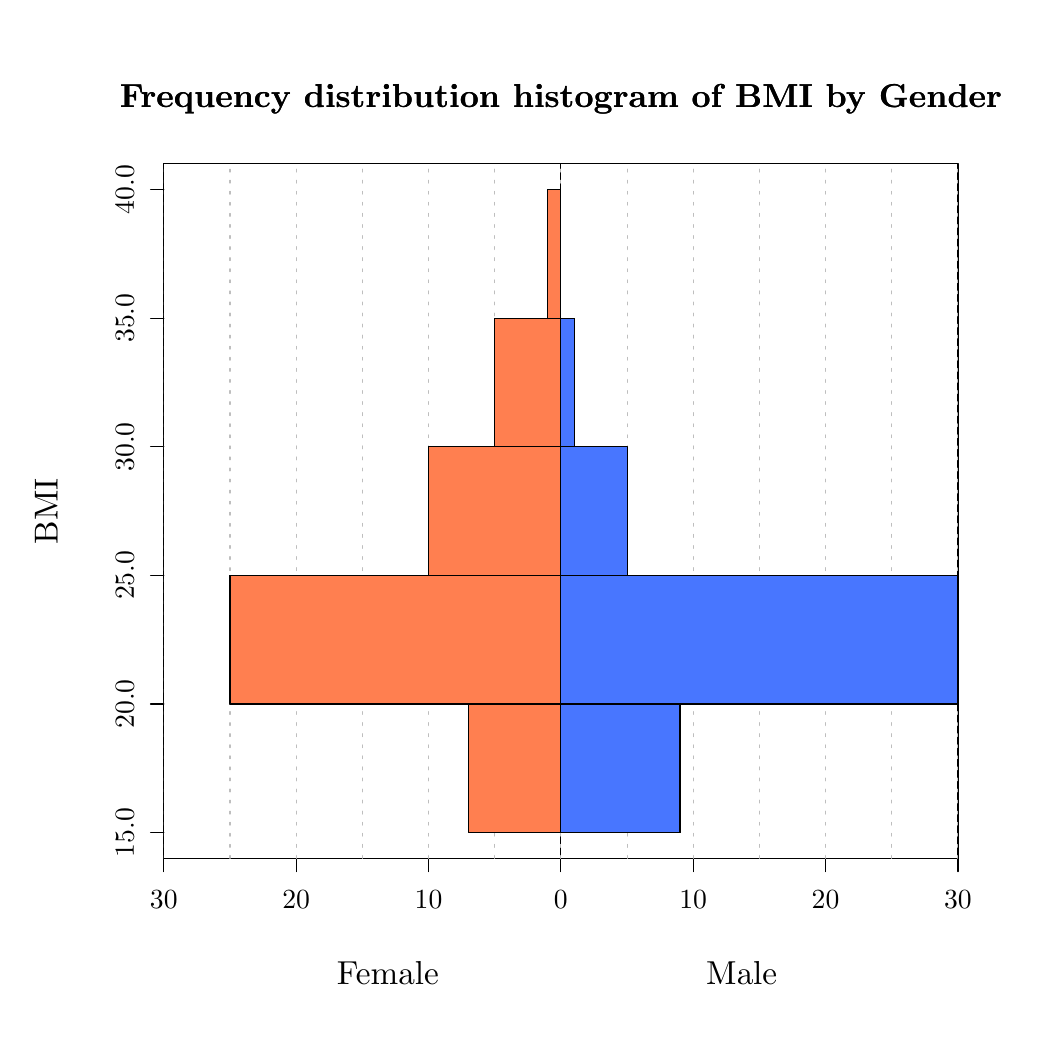
\begin{tikzpicture}[x=1pt,y=1pt]
\definecolor{fillColor}{RGB}{255,255,255}
\path[use as bounding box,fill=fillColor,fill opacity=0.00] (0,0) rectangle (361.35,361.35);
\begin{scope}
\path[clip] (  0.00,  0.00) rectangle (361.35,361.35);
\definecolor{drawColor}{RGB}{0,0,0}

\path[draw=drawColor,line width= 0.4pt,line join=round,line cap=round] (192.68, 70.49) rectangle (159.20,116.97);

\path[draw=drawColor,line width= 0.4pt,line join=round,line cap=round] (192.68,116.97) rectangle ( 73.11,163.44);

\path[draw=drawColor,line width= 0.4pt,line join=round,line cap=round] (192.68,163.44) rectangle (144.85,209.91);

\path[draw=drawColor,line width= 0.4pt,line join=round,line cap=round] (192.68,209.91) rectangle (168.76,256.38);

\path[draw=drawColor,line width= 0.4pt,line join=round,line cap=round] (192.68,256.38) rectangle (187.89,302.86);

\node[text=drawColor,anchor=base,inner sep=0pt, outer sep=0pt, scale=  1.20] at (192.68,332.61) {\bfseries Frequency distribution histogram of BMI by Gender};
\end{scope}
\begin{scope}
\path[clip] (  0.00,  0.00) rectangle (361.35,361.35);
\definecolor{drawColor}{RGB}{0,0,0}

\path[draw=drawColor,line width= 0.4pt,line join=round,line cap=round] (192.68, 70.49) rectangle (235.72,116.97);

\path[draw=drawColor,line width= 0.4pt,line join=round,line cap=round] (192.68,116.97) rectangle (336.15,163.44);

\path[draw=drawColor,line width= 0.4pt,line join=round,line cap=round] (192.68,163.44) rectangle (216.59,209.91);

\path[draw=drawColor,line width= 0.4pt,line join=round,line cap=round] (192.68,209.91) rectangle (197.46,256.38);

\path[draw=drawColor,line width= 0.4pt,line join=round,line cap=round] (192.68,256.38) rectangle (192.68,302.86);

\node[text=drawColor,anchor=base,inner sep=0pt, outer sep=0pt, scale=  1.20] at (192.68,332.61) {\bfseries Frequency distribution histogram of BMI by Gender};
\end{scope}
\begin{scope}
\path[clip] (  0.00,  0.00) rectangle (361.35,361.35);
\definecolor{drawColor}{RGB}{0,0,0}

\path[draw=drawColor,line width= 0.4pt,line join=round,line cap=round] ( 49.20, 61.20) -- (336.15, 61.20);

\path[draw=drawColor,line width= 0.4pt,line join=round,line cap=round] ( 49.20, 61.20) -- ( 49.20, 56.40);

\path[draw=drawColor,line width= 0.4pt,line join=round,line cap=round] ( 97.03, 61.20) -- ( 97.03, 56.40);

\path[draw=drawColor,line width= 0.4pt,line join=round,line cap=round] (144.85, 61.20) -- (144.85, 56.40);

\path[draw=drawColor,line width= 0.4pt,line join=round,line cap=round] (192.68, 61.20) -- (192.68, 56.40);

\path[draw=drawColor,line width= 0.4pt,line join=round,line cap=round] (240.50, 61.20) -- (240.50, 56.40);

\path[draw=drawColor,line width= 0.4pt,line join=round,line cap=round] (288.32, 61.20) -- (288.32, 56.40);

\path[draw=drawColor,line width= 0.4pt,line join=round,line cap=round] (336.15, 61.20) -- (336.15, 56.40);

\node[text=drawColor,anchor=base,inner sep=0pt, outer sep=0pt, scale=  1.00] at ( 49.20, 43.20) {30};

\node[text=drawColor,anchor=base,inner sep=0pt, outer sep=0pt, scale=  1.00] at ( 97.03, 43.20) {20};

\node[text=drawColor,anchor=base,inner sep=0pt, outer sep=0pt, scale=  1.00] at (144.85, 43.20) {10};

\node[text=drawColor,anchor=base,inner sep=0pt, outer sep=0pt, scale=  1.00] at (192.68, 43.20) { 0};

\node[text=drawColor,anchor=base,inner sep=0pt, outer sep=0pt, scale=  1.00] at (240.50, 43.20) {10};

\node[text=drawColor,anchor=base,inner sep=0pt, outer sep=0pt, scale=  1.00] at (288.32, 43.20) {20};

\node[text=drawColor,anchor=base,inner sep=0pt, outer sep=0pt, scale=  1.00] at (336.15, 43.20) {30};

\path[draw=drawColor,line width= 0.4pt,line join=round,line cap=round] ( 49.20, 70.49) -- ( 49.20,302.86);

\path[draw=drawColor,line width= 0.4pt,line join=round,line cap=round] ( 49.20, 70.49) -- ( 44.40, 70.49);

\path[draw=drawColor,line width= 0.4pt,line join=round,line cap=round] ( 49.20,116.97) -- ( 44.40,116.97);

\path[draw=drawColor,line width= 0.4pt,line join=round,line cap=round] ( 49.20,163.44) -- ( 44.40,163.44);

\path[draw=drawColor,line width= 0.4pt,line join=round,line cap=round] ( 49.20,209.91) -- ( 44.40,209.91);

\path[draw=drawColor,line width= 0.4pt,line join=round,line cap=round] ( 49.20,256.38) -- ( 44.40,256.38);

\path[draw=drawColor,line width= 0.4pt,line join=round,line cap=round] ( 49.20,302.86) -- ( 44.40,302.86);

\node[text=drawColor,rotate= 90.00,anchor=base,inner sep=0pt, outer sep=0pt, scale=  1.00] at ( 38.40, 70.49) {15.0};

\node[text=drawColor,rotate= 90.00,anchor=base,inner sep=0pt, outer sep=0pt, scale=  1.00] at ( 38.40,116.97) {20.0};

\node[text=drawColor,rotate= 90.00,anchor=base,inner sep=0pt, outer sep=0pt, scale=  1.00] at ( 38.40,163.44) {25.0};

\node[text=drawColor,rotate= 90.00,anchor=base,inner sep=0pt, outer sep=0pt, scale=  1.00] at ( 38.40,209.91) {30.0};

\node[text=drawColor,rotate= 90.00,anchor=base,inner sep=0pt, outer sep=0pt, scale=  1.00] at ( 38.40,256.38) {35.0};

\node[text=drawColor,rotate= 90.00,anchor=base,inner sep=0pt, outer sep=0pt, scale=  1.00] at ( 38.40,302.86) {40.0};
\end{scope}
\begin{scope}
\path[clip] (  0.00,  0.00) rectangle (361.35,361.35);
\definecolor{drawColor}{RGB}{0,0,0}

\node[text=drawColor,anchor=base,inner sep=0pt, outer sep=0pt, scale=  1.20] at (130.14, 15.60) {Female};

\node[text=drawColor,anchor=base east,inner sep=0pt, outer sep=0pt, scale=  1.20] at (270.83, 15.60) {Male};

\node[text=drawColor,rotate= 90.00,anchor=base,inner sep=0pt, outer sep=0pt, scale=  1.20] at ( 10.80,186.67) {BMI};
\end{scope}
\begin{scope}
\path[clip] ( 49.20, 61.20) rectangle (336.15,312.15);
\definecolor{drawColor}{RGB}{0,0,0}

\path[draw=drawColor,line width= 0.4pt,line join=round,line cap=round] (192.68, 61.20) -- (192.68,312.15);
\end{scope}
\begin{scope}
\path[clip] (  0.00,  0.00) rectangle (361.35,361.35);
\definecolor{drawColor}{RGB}{0,0,0}

\path[draw=drawColor,line width= 0.4pt,line join=round,line cap=round] ( 49.20, 61.20) --
	(336.15, 61.20) --
	(336.15,312.15) --
	( 49.20,312.15) --
	( 49.20, 61.20);
\end{scope}
\begin{scope}
\path[clip] ( 49.20, 61.20) rectangle (336.15,312.15);
\definecolor{drawColor}{RGB}{190,190,190}

\path[draw=drawColor,line width= 0.4pt,dash pattern=on 1pt off 3pt ,line join=round,line cap=round] (  1.38, 61.20) -- (  1.38,312.15);

\path[draw=drawColor,line width= 0.4pt,dash pattern=on 1pt off 3pt ,line join=round,line cap=round] ( 25.29, 61.20) -- ( 25.29,312.15);

\path[draw=drawColor,line width= 0.4pt,dash pattern=on 1pt off 3pt ,line join=round,line cap=round] ( 49.20, 61.20) -- ( 49.20,312.15);

\path[draw=drawColor,line width= 0.4pt,dash pattern=on 1pt off 3pt ,line join=round,line cap=round] ( 73.11, 61.20) -- ( 73.11,312.15);

\path[draw=drawColor,line width= 0.4pt,dash pattern=on 1pt off 3pt ,line join=round,line cap=round] ( 97.03, 61.20) -- ( 97.03,312.15);

\path[draw=drawColor,line width= 0.4pt,dash pattern=on 1pt off 3pt ,line join=round,line cap=round] (120.94, 61.20) -- (120.94,312.15);

\path[draw=drawColor,line width= 0.4pt,dash pattern=on 1pt off 3pt ,line join=round,line cap=round] (144.85, 61.20) -- (144.85,312.15);

\path[draw=drawColor,line width= 0.4pt,dash pattern=on 1pt off 3pt ,line join=round,line cap=round] (168.76, 61.20) -- (168.76,312.15);

\path[draw=drawColor,line width= 0.4pt,dash pattern=on 1pt off 3pt ,line join=round,line cap=round] (192.68, 61.20) -- (192.68,312.15);

\path[draw=drawColor,line width= 0.4pt,dash pattern=on 1pt off 3pt ,line join=round,line cap=round] (216.59, 61.20) -- (216.59,312.15);

\path[draw=drawColor,line width= 0.4pt,dash pattern=on 1pt off 3pt ,line join=round,line cap=round] (240.50, 61.20) -- (240.50,312.15);

\path[draw=drawColor,line width= 0.4pt,dash pattern=on 1pt off 3pt ,line join=round,line cap=round] (264.41, 61.20) -- (264.41,312.15);

\path[draw=drawColor,line width= 0.4pt,dash pattern=on 1pt off 3pt ,line join=round,line cap=round] (288.32, 61.20) -- (288.32,312.15);

\path[draw=drawColor,line width= 0.4pt,dash pattern=on 1pt off 3pt ,line join=round,line cap=round] (312.24, 61.20) -- (312.24,312.15);

\path[draw=drawColor,line width= 0.4pt,dash pattern=on 1pt off 3pt ,line join=round,line cap=round] (336.15, 61.20) -- (336.15,312.15);

\path[draw=drawColor,line width= 0.4pt,dash pattern=on 1pt off 3pt ,line join=round,line cap=round] (360.06, 61.20) -- (360.06,312.15);
\end{scope}
\begin{scope}
\path[clip] (  0.00,  0.00) rectangle (361.35,361.35);
\definecolor{drawColor}{RGB}{0,0,0}
\definecolor{fillColor}{RGB}{255,127,80}

\path[draw=drawColor,line width= 0.4pt,line join=round,line cap=round,fill=fillColor] (192.68, 70.49) rectangle (159.20,116.97);

\path[draw=drawColor,line width= 0.4pt,line join=round,line cap=round,fill=fillColor] (192.68,116.97) rectangle ( 73.11,163.44);

\path[draw=drawColor,line width= 0.4pt,line join=round,line cap=round,fill=fillColor] (192.68,163.44) rectangle (144.85,209.91);

\path[draw=drawColor,line width= 0.4pt,line join=round,line cap=round,fill=fillColor] (192.68,209.91) rectangle (168.76,256.38);

\path[draw=drawColor,line width= 0.4pt,line join=round,line cap=round,fill=fillColor] (192.68,256.38) rectangle (187.89,302.86);
\definecolor{fillColor}{RGB}{72,118,255}

\path[draw=drawColor,line width= 0.4pt,line join=round,line cap=round,fill=fillColor] (192.68, 70.49) rectangle (235.72,116.97);

\path[draw=drawColor,line width= 0.4pt,line join=round,line cap=round,fill=fillColor] (192.68,116.97) rectangle (336.15,163.44);

\path[draw=drawColor,line width= 0.4pt,line join=round,line cap=round,fill=fillColor] (192.68,163.44) rectangle (216.59,209.91);

\path[draw=drawColor,line width= 0.4pt,line join=round,line cap=round,fill=fillColor] (192.68,209.91) rectangle (197.46,256.38);

\path[draw=drawColor,line width= 0.4pt,line join=round,line cap=round,fill=fillColor] (192.68,256.38) rectangle (192.68,302.86);
\end{scope}
\end{tikzpicture}
}
\end{center}

\begin{enumerate}
\item Draw the pie chart for the gender.
\item In which group is more representative the mean of the BMI?
\item Calculate the mean for the whole sample.
\end{enumerate}
Use the following sums\\
Females: $\sum x_in_i = 1160$ kg/m$^2$ \quad $\sum x_i^2n_i = 29050$ kg$^2$/m$^4$\\
Males: $\sum x_in_i = 1002$ kg/m$^2$ \quad $\sum x_i^2n_i = 22781$ kg$^2$/m$^4$
}
%SOLUTION
{\begin{enumerate}[start=2]
\item $\bar{f} =24.17$ kg/m$^2$, $s_{f}^2=21.1806$ (kg/m$^2$)$^2$, $s_f=4.6$ kg/m$^2$ and $cv_f = 0.19$.\\
$\bar{m} =22.28$ kg/m$^2$, $s_{m}^2=9.9506$ (kg/m$^2$)$^2$, $s_m=3.15$ kg/m$^2$ and $cv_m = 0.14$.
Thus, the mean of males is more representative.
\item $\bar{x}=23.25$ kg/m$^2$.
\end{enumerate}
}
%RESOLUTION
{Lamemos $H$ a la variable que mide el índice de masa corporal para los hombres y $M$ para las mujeres.
\begin{enumerate}
\item A partir del histograma de frecuencias absolutas de las mujeres podemos obtener fácilmente las frecuencias absolutas de los intervalos mirando la altura de las barras, y a partir de las frecuencias absolutas podemos calcular el resto de frecuencias.
La tabla de frecuencias para las mujeres es:
\[
\begin{array}{|c|r|r|r|r|}
\hline
   M   & n_i &  f_i & N_i &  F_i \\
\hline
 15-20 &   7 & 0.15 &   7 & 0.15 \\
 20-25 &  25 & 0.52 &  32 & 0.67 \\
 25-30 &  10 & 0.21 &  42 & 0.88 \\
 30-35 &   5 & 0.10 &  47 & 0.98 \\
 35-40 &   1 & 0.02 &  48 & 1.00 \\
\hline
\mbox{Suma} & 48 & 1.00 & & \\
\hline
\end{array}
\]
Del mismo modo, a partir del histograma de frecuencias absolutas de los hombres obtenemos la tabla de frecuencias para hombres:
\[
\begin{array}{|c|r|r|r|r|}
\hline
   H   & n_i &  f_i & N_i &  F_i \\
\hline
 15-20 &   9 & 0.20 &   9 & 0.20 \\
 20-25 &  30 & 0.67 &  39 & 0.87 \\
 25-30 &   5 & 0.11 &  44 & 0.98 \\
 30-35 &   1 & 0.02 &  45 & 1.00 \\
\hline
\mbox{Suma} & 45 & 1.00 & & \\
\hline
\end{array}
\]

\item La variable Sexo sólo tiene dos categorías que son Hombre y Mujer, de modo que el diagrama de sectores asociado sólo tendrá dos sectores. La tabla de frecuencias de la variable sexo es:
\[
\begin{array}{|c|r|r|}
\hline
  \textrm{Sexo}  & n_i &   f_i \\
\hline
 \textrm{Mujer}  &  48 & 0.516 \\
\hline
 \textrm{Hombre} &  45 & 0.484 \\
\hline
  \textrm{Suma}  &  93 & 1.000 \\
\hline
\end{array}
\]
Así pues, para calcular el ángulo correspondiente a cada sector basta con multiplicar $360^{\circ}$ (el ángulo de la circunferencia completa) por la frecuencia relativa de cada categoría:
\[
\alpha_m=360^{\circ}0.516=186^{\circ}\qquad \alpha_h=360^{\circ}0.484=174^{\circ}.
\]
Y el diagrama de sectores asociados es:
\begin{center}
\includegraphics[scale=0.6]{img/sectores-des-29}
\end{center}

\item La media será más representativa en el grupo que tenga menos dispersión, y para comparar la dispersión de ambos grupos necesitamos el coeficiente de variación.
Calculamos para ello los estadísticos necesarios a partir de las tablas de frecuencias. Para las mujeres tenemos:
\[
\begin{array}{|c|r|r|r|r|}
\hline
   M   & m_i & n_i & m_in_i & m_i^2n_i \\
\hline
 15-20 & 17.5 &  7 & 122.5 & 2143.75 \\
 20-25 & 22.5 & 25 & 562.5 & 12656.25\\
 25-30 & 27.5 & 10 & 275.0 & 7562.50 \\
 30-35 & 32.5 &  5 & 162.5 & 5281.25 \\
 35-40 & 37.5 &  1 &  37.5 & 1406.25 \\
\hline
\mbox{Suma} & & 48 & 1160.0& 29050.00 \\
\hline
\end{array}
\]

\begin{align*}
\bar{m} & = \frac{\sum m_{i}}{n_m}=\frac{1160}{48}=24.17,  \\
s_{m}^2 &= \frac{\sum m_{i}^2}{n_m}-\bar{m}^2 = \frac{29050}{48}-24.17^2=21.1806,  \\
s_m &= \sqrt{21.1806} = 4.6,\\
cv_m &= \frac{s_m}{|\bar{m}|}=\frac{4.6}{24.17} = 0.19.
\end{align*}

Y para los hombres:
\[
\begin{array}{|c|r|r|r|r|}
\hline
   H   & h_i &  n_i & h_in_i &  h_i^2n_i \\
\hline
 15-20 &  17.5 &  9 & 157.5 &  2756.25 \\
 20-25 &  22.5 & 30 & 675.0 & 15187.50 \\
 25-30 &  27.5 &  5 & 137.5 &  3781.25 \\
 30-35 &  32.5 &  1 &  32.5 &  1056.25 \\
\hline
\mbox{Suma} & & 45 & 1002.5 & 22781.25 \\
\hline
\end{array}
\]

\begin{align*}
\bar{h} & = \frac{\sum h_{i}}{n_h}=\frac{1002.5}{45}=22.28,  \\
s_{h}^2 & = \frac{\sum h_{i}^2}{n_h}-\bar{h}^2 =
\frac{22781.25}{45}-22.28^2=9.9506,  \\
s_h &= \sqrt{9.9506} = 3.15,\\
cv_h &= \frac{s_h}{|\bar{h}|}=\frac{3.15}{22.28} = 0.14.
\end{align*}

Así pues, ambas muestras tienen un coeficiente de variación bajo y por tanto las medias son muy representativas, pero lo es un poco más la de los hombres ya que tienen una poca menos dispersión.

\item Para calcular la media de toda la muestra podemos hacer una media ponderada de las medias de las mujeres y l
os hombres donde los pesos son los tamaños muestrales de cada grupo.
\[
\bar{x}=\frac{p_m\bar{m}+p_h\bar{h}}{p_m+p_h}=\frac{45\cdot 22.28+48\cdot 24.17}{45+48}=23.25.
\]

\end{enumerate}
}


\newproblem*{des-30}{med}{*}
%STATEMENT
{Se ha medido el tiempo necesario, en días, para curar un tipo concreto de infección (tiempo transcurrido desde el comienzo del tratamiento hasta el alta) en dos grupos de pacientes a los que se han aplicado antibióticos diferentes.
En un grupo de 80 pacientes tratados con el antibiótico A, los resultados obtenidos fueron:
\[
\begin{array}{|c|c|}
\hline
\mbox{Tiempo (días)} & n_i \\
\hline
{[0,30)} & 50 \\
{[30,60)} & 20 \\
{[60,90)} & 10 \\
\hline
\end{array}
\]

Mientras que en un grupo de 100 pacientes tratados con el antibiótico B se obtuvo:
\[
\begin{array}{|c|c|}
\hline
\mbox{Tiempo (días)} & n_i \\
\hline
{[0,30)} & 40 \\
{[30,60)} & 50 \\
{[60,90)} & 10 \\
\hline
\end{array}
\]

\begin{enumerate}
\item Calcular la media y la desviación típica del número de días hasta el alta, para cada uno de los antibióticos.
\item ¿En qué antibiótico es más representativa la media?. Justificar la respuesta numéricamente.
\item ¿Cuánto vale el percentil 90 del tiempo de curación para los pacientes tratados con B?
\item ¿Qué tiempo de recuperación ha sido relativamente más alto, uno de 40 días de un paciente tratado con A, o uno de 45 días de otro tratado con B? Justificar la respuesta numéricamente.
\end{enumerate}
}


\newproblem{des-31}{med}{*}
%STATEMENT
{Para  estudiar la eficacia de un nuevo fármaco en el tratamiento de la hipertensión arterial, se tomaron los valores
de la tensión arterial diastólica (TAD) en 8 pacientes antes del tratamiento ($X$) y después de un mes de tratamiento
($Y$), obteniéndose los siguientes resultados:
\begin{center}
\begin{tabular}{|c|r|r|r|r|r|r|r|r|}
\hline
$X$ & 100 & 104 & 96 & 98 & 105 & 106 & 110 & 100 \\
\hline
$Y$ & 92 & 97 & 94 & 100 & 94 & 92 & 95 & 104 \\
\hline
\end{tabular}
\end{center}

\begin{enumerate}
\item ¿En qué variable es más representativa la media?
\item Hallar el coeficiente de asimetría de la variable $Y$ e interpretarlo.
\end{enumerate}
}
%SOLUTION
{\begin{enumerate}
\item $\bar x=102.375$, $s_x^2=18.9844$, $s_x=4.3571$ y $cv_x =0.0426$.\\
$\bar y=96$, $s_y^2=15.25$, $s_y=3.9051$ y $cv_y = 0.0407$.\\
Como ambos coeficientes de variación son casi iguales podemos concluir que ambas medias son igual de representativas.
\item $g_1=0.9068$ lo que indica que es asimétrica hacia la derecha.
\end{enumerate}
}
%RESOLUTION
{\begin{enumerate}
\item Para ver en qué muestra es más representativa la media tenemos que comparar las dispersiones de ambas muestras mediante el coeficiente de variación. Para ello, procedemos al cálculo de los estadísticos necesarios:
\begin{align*}
\bar{x} & = \frac{\sum x_{i}}{n}=\frac{100+\cdots+100}{8}=\frac{819}{8}=102.375,  \\
s_{x}^2 & = \frac{\sum x_{i}^2}{n}-\bar{x}^2 =
\frac{100^2+\cdots+100^2}{8}-102.375^2=\frac{83997}{8}-10480,6406=18.9844,  \\
s_{x} & = \sqrt{18.9844}=4.3571,  \\
cv_x &= \frac{s_x}{|\bar{x}|}= \frac{4.3571}{102.375}=0.0426,\\
\bar{y} & = \frac{\sum y_{j}}{n}=\frac{92+\cdots+104}{8}=
\frac{768}{8}=96,  \\
s_{y}^2 & = \frac{\sum y_{j}^2}{n}-\bar{y}^2 =
\frac{92^2+\cdots+104^2}{8}-96^2=\frac{73850}{8}-9216=15.25,  \\
s_{y} & = \sqrt{15.25}=3.9051,  \\
cv_y &= \frac{s_y}{|\bar{y}|}= \frac{3.9051}{96}=0.0407,\\
\end{align*}
Ambos coeficientes de variación son muy pequeños, lo cual indica que hay muy poca dispersión en las muestras y las medias son muy representativas, aunque un poco más la de $Y$ por tener un coeficiente de variación más pequeño.

\item El coeficiente de asimetría de $Y$ es
\[g_1=\frac{\sum(y_j-\bar{y})^3/n}{s_y^3}=
\frac{\left((92-96)^3+\cdots +(104-96)^3\right)/8}{3.9051^3}=\frac{432/8}{59,552}=0.9068,\]
lo que indica que la distribución es asimétrica a la derecha aunque no los suficiente como para rechazar la hipótesis de que los datos provienen de una población normal.
\end{enumerate}
}


\newproblem{des-32}{amb}{*}
%STATEMENT
{Una piscifactoría realiza un estudio para determinar si una especie de pez está en peligro extinción en los ríos de una región.
Para ello se midió el número de peces en 10 sitios diferentes obteniendo los siguientes resultados en unidades
por hectómetro cúbico:
\begin{center}
  36 -- 11 -- 7 -- 18 -- 35 -- 27 -- 21 -- 15 -- 25 -- 12
\end{center}
Se pide:
\begin{enumerate}
\item Calcular las medidas de tendencia central.
\item Calcular el coeficiente de apuntamiento e interpretarlo.
\end{enumerate}
}
%SOLUTION
{\begin{enumerate}
\item $\bar{x} = 20.7$ peces, $Me=19.5$ peces, no hay moda porque todos los valores tienen frecuencia 1.
\item $g_2= -1.13$ lo que indica que es una distribución bastante platicúrtica.
\end{enumerate}
}
%RESOLUTION
{Llamemos $X$ al número de peces por hectómetro cúbico.
\begin{enumerate}
\item Las medidas de tendencia central son la media aritmética, la mediana y la moda. Calculamos primero la media:
\[
\bar{x} = \frac{\sum x_{i}}{n}=\frac{36+\cdots+12}{10}=\frac{207}{10}=20.7 \mbox{ peces},
\]

Para calcular la mediana ordenamos los valores de la muestra:
\begin{center}
  7 -- 11 -- 12 -- 15 -- 18 -- 21 -- 25 -- 27 -- 35 -- 36
\end{center}
Como el tamaño de la muestra es par, habrá dos individuos que ocupen las posiciones centrales de la muestra, y estos serán los que ocupen las posiciones $n/2=10/2=5$ y $n/2+1=6$, es decir, los valores 18 y 21. Así pues la mediana es
\[
Me=\frac{18+21}{2}=19.5 \mbox{ peces}.
\]

Por último, no podemos decir que haya moda porque todos los valores tienen frecuencia 1.

\item La fórmula del coeficiente de apuntamiento es
\[
g_2=\frac{\sum (x_i-\bar{x})^4}{ns^4}-3,
\]
así que necesitamos calcular previamente la desviación típica:
\begin{align*}
s^2 & = \frac{\sum x_{i}^2}{n}-\bar{x}^2 =
\frac{36^2+\cdots+12^2}{10}-20.7^2=\frac{5179}{10}-428,49=89.41,\\
s &=\sqrt{89.41}=9.4557.
\end{align*}
Así pues, tenemos
\[
g_2=\frac{(36-20.7)^4+\cdots + (12-20.7)^4}{10\cdot 9.4557^4}-3=\frac{149449.657}{79941,9504}-3=-1.13,
\]
lo que indica que la distribución es bastante platicúrtica, es decir, con menos apuntamiento que una distribución normal.
\end{enumerate}
}


\newproblem{des-33}{amb}{*}
%STATEMENT
{Las temperaturas (en ºC) observadas en Barcelona y La Coruña en 12 días elegidos aleatoriamente el último año fueron:
\begin{center}
\begin{tabular}{|l|cccccccccccc|}
\hline
Barcelona & 13 & 14 & 16 & 18 & 21 & 25 & 28 & 28 & 25 & 21 & 17 & 13\\ \hline
La Coruña & 13 & 13 & 15 & 16 & 17 & 20 & 22 & 23 & 22 & 19 & 15 & 13\\ \hline
\end{tabular}
\end{center}
Se pide:

\begin{enumerate}
\item ¿En cuál de las dos ciudades hay mayor variación de temperaturas?
\item ¿Por debajo de qué valor estarán las temperaturas de la mitad de los días en ambas ciudades?
\end{enumerate}
}
%SOLUTION
{\begin{enumerate}
\item $cv_b = 0.2684$ y $cv_c =0.2071$ lo que indica que hay una ligera mayor variación de temperaturas en Barcelona.
\item $Me_b = 19,5.$ y $Me_c= 16.5$.
\end{enumerate}
}
%RESOLUTION
{Llamemos $B$ a la variable que mide las temperaturas en Barcelona, y $C$ a la que mide las temperaturas en La Coruña.
\begin{enumerate}
\item Para ver en qué ciudad hay mayor variación de temperatura tenemos que calcular los coeficientes de variación de ambas ciudades y compararlos.
\begin{align*}
\bar{b} &=\frac{\sum b_i}{n}= \frac{13+14+\cdots+13}{12}=\frac{239}{12}=19.9167,\\
s_b^2 &= \frac{\sum b_i^2}{n}-\bar{b}^2=\frac{13^2+14^2+\cdots+13^2}{12}-19.9167^2=\frac{5103}{12}-396.6749=28.5764,\\
s_b &=\sqrt{28.5764}=5.3457,\\
cv_b &= \frac{s_b}{|\bar{b}|}=\frac{5.3457}{19.9167}=0.2684,\\
\bar{c} &=\frac{\sum c_i}{n}= \frac{13+13+\cdots+13}{12}=\frac{208}{12}=17.3333,\\
s_c^2 &= \frac{\sum c_i^2}{n}-\bar{c}^2=\frac{13^2+13^2+\cdots+13^2}{12}-17.3333^2=\frac{3760}{12}-300.4433=12.8889,\\
s_c &=\sqrt{12.8889}=3.5901,\\
cv_c &= \frac{s_c}{|\bar{c}|}=\frac{3.5901}{17.3333}=0.2071.
\end{align*}
Por consiguiente, como el coeficiente de variación es mayor en Barcelona, es en esta ciudad donde hay mayor variación de temperaturas.

\item El valor que cumple que por debajo del mismo están la mitad de los valores de la muestra es la mediana.
Para calcular la mediana en ambas ciudades ordenamos los valores de la muestra de menor a mayor, y puesto que tenemos un tamaño muestral par $n=12$, buscamos los dos valores centrales, que ocuparan las posiciones $n/2=6$ y $n/2+1=7$.
En el caso de Barcelona tenemos que dichos valores son
\begin{center}
\begin{tabular}{|c|cccccccccccc|}
\hline
Posición & 1 & 2 & 3 & 4 & 5 & 6 & 7 & 8 & 9 & 10 & 11 & 12   \\ \hline
B & 13 & 13 & 14 & 16 & 17 & \fbox{18} & \fbox{21} & 21 & 25 & 25 & 28 & 28 \\ \hline
\end{tabular}
\end{center}
Como son valores diferentes, la mediana es $Me_b=\dfrac{18+21}{2}=19,5.$

En el caso de La Coruña tenemos
\begin{center}
\begin{tabular}{|c|cccccccccccc|}
\hline
Posición & 1 & 2 & 3 & 4 & 5 & 6 & 7 & 8 & 9 & 10 & 11 & 12   \\ \hline
C & 13 & 13 & 13 &  15 & 15 & \fbox{16} & \fbox{17} & 19 & 20 & 22 & 22 & 23 \\ \hline
\end{tabular}
\end{center}
Y al igual que antes, la mediana es $Me_c=\dfrac{16+17}{2}=16,5.$
\end{enumerate}
}


\newproblem{des-34}{gen}{*}
%STATEMENT
{Las pruebas de determinación del cociente intelectual realizadas en un colectivo de alumnos universitarios
reflejan los siguientes resultados:
\begin{center}
\begin{tabular}{|c|c|}
\hline
   C.I.    & Nº de alumnos \\
\hline
  [80,90)  &       3       \\
\hline
 [90,100)  &      12       \\
\hline
 [100,110) &      21       \\
\hline
 [110,120) &      24       \\
\hline
 [120,130) &      13       \\
\hline
 [130,140) &       2       \\
\hline
\end{tabular}
\end{center}
\begin{enumerate}
\item Calcular el coeficiente de variación del cociente intelectual. ¿Es representativa la media?
\item Si se considera ``muy inteligente'' a una persona cuyo cociente intelectual se encuentra en el 10\% de los más inteligentes, ¿cuál será el cociente que delimita la categoría ``muy inteligente'' en el colectivo de alumnos?
\end{enumerate}
}
%SOLUTION
{\begin{enumerate}
\item $cv=0.1$ lo que indica que hay poca dispersión y la media es muy representativa.
\item $P_{90}=125.77$.
\end{enumerate}
}
%RESOLUTION
{\begin{enumerate}
\item Para calcular el coeficiente de variación necesitamos la media y la desviación típica.
Para facilitar los cálculos, añadimos dos nuevas columnas a la tabla de distribución de frecuencias:
\[
\begin{array}{|c|c|r|r|r|}
\hline
   \textrm{C.I.}   & x_i & \multicolumn{1}{c|}{n_i} & \multicolumn{1}{c|}{x_in_i} & \multicolumn{1}{c|}{x_i^2n_i}\\
\hline\hline
  [80,90)  &  85  &   3       & 255 & 21675 \\
\hline
 [90,100)  &  95 &    12       & 1140 & 108300 \\
\hline
 [100,110) &  105 &    21       & 2205 & 231525\\
\hline
 [110,120) &  115 &    24       & 2760 & 317400\\
\hline
 [120,130) &  125 &    13       & 1625 & 203125\\
\hline
 [130,140) &  135 &     2       & 270 & 36450\\
\hline\hline
 \textrm{Sumas} &  & 75 & 8255 & 918475 \\
\hline
\end{array}
\]
A partir de aquí calculamos los estadísticos que necesitamos.
\begin{align*}
\bar{x} & = \frac{\sum x_in_i}{N}=\frac{8255}{75}=110.07,\\
s^2 & =\frac{\sum x_i^2n_i}{N}-\bar{x}^2= \frac{918475}{75}-110.07^2=131.6622,\\
s & =\sqrt{131.6622}=11.47.
\end{align*}
Finalmente calculamos el coeficiente de variación:
\[
cv=\frac{s}{|\bar{x}|}=\frac{11.47}{110.07}= 0.1.
\]
Puesto que el coeficiente de variación es pequeño, podemos concluir que hay poca dispersión en la muestra y por tanto, la media es representativa.

\item Buscamos el coeficiente intelectual por encima del cual está el 10\% más inteligente de la clase, o lo que es lo mismo, por debajo del cual está el 90\% menos inteligente de la clase. En definitiva se trata de calcular el percentil 90.
Para ello necesitamos la columna de frecuencias acumuladas en la tabla
\[
\begin{array}{|c|r|r|}
\hline
   \textrm{C.I.}    & \multicolumn{1}{c|}{n_i} & \multicolumn{1}{c|}{N_i} \\
\hline\hline
  [80,90)  &       3       & 3 \\
\hline
 [90,100)  &      12       & 15 \\
\hline
 [100,110) &      21       & 36 \\
\hline
 [110,120) &      24       & 60 \\
\hline
 [120,130) &      13       & 73 \\
\hline
 [130,140) &       2       & 75 \\
\hline
\end{array}
\]

La frecuencia acumulada correspondiente al percentil 90 es $N_{P_{90}}=90\cdot 75/100=67.5$. Mirando el la  columna de frecuencias acumuladas de la tabla de frecuencias comprobamos que dicha frecuencia se alcanza dentro del intervalo $[120,130)$.
Interpolando en este intervalo obtenemos el percentil que buscamos \[P_{90}=120+\frac{67.5-60}{13}10=125.77.\]
\end{enumerate}
}


\newproblem{des-35}{far}{*}
%STATEMENT
{En un laboratorio farmacéutico se van a fabricar dos tipos de cápsulas $A$ y $B$, cuyos contenidos en principio
activo debe ser 250 y 500 mg. respectivamente. Para ello se prueban dos máquinas dosificadoras, una para cada tipo de
cápsulas, siendo los contenidos en principio activo de las cápsulas fabricadas con ellas los siguientes:
\[
\begin{array}{c|c}
A & B  \\ \hline
238 & 488  \\
245 & 494  \\
236 & 476  \\
248 & 483  \\
241 & 492  \\
243 &
\end{array}
 \]
¿En cuál de las dos máquinas es más representativa la media?
Razonar la respuesta.
}
%SOLUTION
{$cv_{A} = 0.0167$ y $cv_{B}=0.0133$, luego es un poco más representativa la media en la máquina $B$.
}
%RESOLUTION
{Llamaremos $A$ a la variable que mide la cantidad de principio activo que pone la máquina $A$ en cada cápsula y $B$ a la variable que mide la cantidad de principio activo que pone la máquina $B$ en cada cápsula.
Para ver en cual de las dos muestras es más representativa la media, tenemos que calcular los coeficientes de variación en cada caso.

Calculamos primero los estadísticos necesarios para la máquina $A$:
\begin{align*}
\bar{A} & = \frac{\sum A_{i}}{n_{A}}=\frac{1451}{6}=241.833,\\
s_{A}^2 & =  \frac{\sum{A_{i}^2}{n_{A}}}-\bar{A}^2= \frac{350999}{6}-241.833^2=16.472,\\
s_{A} & = \sqrt{16.472}= 4.058,\\
cv_{A} & = \frac{s_{A}}{\bar{A}}=\frac{4.058}{241.833}=0.0167,
\end{align*}

En el caso de la máquina $B$ tenemos:
\begin{align*}
\bar{B} & = \frac{\sum B_{i}}{n_{B}}=\frac{2433}{5}=486.6,\\
s_{B}^2 & = \frac{\sum{B_{i}^2}{n_{B}}}-\bar{B}^2= \frac{1184109}{5}-486.6^2=42.24,\\
s_{B} & = \sqrt{42.24}= 6.499,\\
cv_{B} & = \frac{s_{B}}{\bar{B}}=\frac{6.499}{486.6}=0.0133.
\end{align*}

Como el coeficiente de variación de la muestra de $B$ es un poco menor que el de $A$, la dispersión será menor en la muestra de $B$ y $\bar{B}$ será un poco más representativa que $\bar{A}$.
}


\newproblem{des-36}{gen}{*}
%STATEMENT
{En un centro de reclutamiento se han medido las alturas de 150 jóvenes, obteniéndose la siguiente tabla de frecuencias:
\[
\begin{tabular}{|c|c|}
\hline
Altura: & Número de jóvenes: \\ \hline
1.50-1.60 & 12 \\ \hline
1.60-1.70 & 30 \\ \hline
1.70-1.80 & 52 \\ \hline
1.80-1.90 & 42 \\ \hline
1.90-2.00 & 11 \\ \hline
2.00-2.10 & 3 \\ \hline
\end{tabular}
\]

\begin{enumerate}
\item Calcular el coeficiente de variación. ¿Es representativa la media?
\item  Si se considera alto a un joven cuya altura corresponde como mínimo a la del percentil 85, ¿cuál es la
mínima altura que tendrá un alto?
\end{enumerate}
}
%SOLUTION
{\begin{enumerate}
\item $cv=0.065$ lo que indica muy poca dispersión y una media muy representativa.
\item $ P_{85}=1.88$ mt.
\end{enumerate}
}
%RESOLUTION
{\begin{enumerate}
\item  El coeficiente de variación se define como
\[
cv=\dfrac{s}{|\bar{x}|},
\]
de modo que necesitamos calcular la media y la desviación típica, pero antes de nada, completamos la tabla de frecuencias.
\[
\begin{array}{|c|c|c|c|c|}
\hline
x_{i} & n_{i} & N_{i} & x_{i}n_{i} & x_{i}^2n_{i}\\ \hline
1.50-1.60 & 12 & 12 & 18.6 & 28.83 \\
1.60-1.70 & 30 & 42 & 49.5 & 81.68 \\
1.70-1.80 & 52 & 94 & 91 & 159.25\\
1.80-1.90 & 42 & 136 & 77.7 & 143.75\\
1.90-2.00 & 11 & 147 & 21.45 & 41.83\\
2.00-2.10 & 3 & 150 & 6.15 & 12.61\\ \hline
\mbox{Sumas} & 150 & & 264.4 & 467.94 \\
\hline
\end{array}
\]
Ahora calculamos la media y la desviación típica:
\begin{eqnarray*}
\bar{x} & = & \frac{\sum
x_{i}n_{i}}{N}=\frac{264.4}{150}=1.7627.\\
s^2 & = & \frac{\sum x_{i}^2 n_{i}}{N}-\bar{x}^2 =
\frac{467.94}{150}-1.7627^2=0.013.\\
s & = & \sqrt{0.02}=0.114.
\end{eqnarray*}
Por consiguiente, el coeficiente de variación es
\[ cv=\frac{0.114}{1.7627}=0.065, \]
lo que indica que hay muy poca dispersión y la media es muy representativa.

\item Tenemos que calcular el percentil 85 para ver a partir de qué estatura un joven es considerado alto.
La frecuencia absoluta acumulada correspondiente al percentil 85 es $85\cdot N/100=85\cdot 150/100 = 127.5$.
Mirando la tabla de frecuencias en la columna de las frecuencias absolutas acumuladas podemos comprobar que la frecuencia 127.5 se alcanza en algún punto del intervalo 1.80-1.90.
Para obtener el percentil 85 interpolamos en dicho intervalo:
\[ P_{85}=1.80+\frac{127.5-94}{42}(1.90-1.80)=1.88. \]
\end{enumerate}
}


\newproblem{des-37}{med}{*}
%STATEMENT
{Se ha realizado un estudio sobre la tensión arterial en dos ciudades A y B. Se tomó una muestra de 20 individuos, que arrojó los siguientes valores:
\begin{center}
\begin{tabular}{l}
\begin{tabular}{|l|c|c|c|c|c|c|c|c|c|c|}
\hline
 Tensión & 135 & 128 & 137 & 110 & 154 & 142 & 121 & 127 & 114 & 103 \\
\hline
 Ciudad  &  A  &  B  &  A  &  B  &  A  &  A  &  A  &  B  &  B  &  B  \\
\hline
\end{tabular}
\\[.5cm]
\begin{tabular}{|l|c|c|c|c|c|c|c|c|c|c|}
\hline
 Tensión & 98 & 96 & 114 & 123 & 132 & 141 & 132 & 121 & 98 & 136 \\
\hline
 Ciudad  & A  & B  &  A  &  B  &  A  &  B  &  A  &  B  & B  &  A  \\
\hline
\end{tabular}
\end{tabular}
\end{center}
Se pide:
\begin{enumerate}
\item Construir la tabla de frecuencias para la tensión, agrupando en clases de amplitud 10, entre 95 y 155.
\item Dibujar el polígono de frecuencias acumuladas correspondiente a la tabla anterior.
\item Calcular el coeficiente de asimetría e interpretarlo.
\item Calcular el tercer decil e interpretarlo.
\item Considerando los datos sin agrupar, ¿en qué ciudad son más homogéneas las tensiones?
\end{enumerate}
}
%SOLUTION
{\begin{enumerate}[start=3]
\item $\bar x = 123$ mmHg, $s^2= 251$ mmHg$^2$, $s=15.843$ mmHg y $g_1=-0.12$, por lo que la distribución es un poco asimétrica hacia la izquierda.
\item $D_3= 111,67$ mmHg.
\item $\bar x_A=130.1$ mmHg, $s^2_A=219.89$ mmHg$^2$, $s_A=14.8287$ mmHg y $cv_A =0.1139$.\\
$\bar x_B=116.1$ mmHg, $s^2_B=189.69$ mmHg$^2$, $s_B=13.7728$ mmHg y y $cv_B = 0.1186$.
Así pues, como el $cv_A<cv_B$ las tensiones son un poco más homogéneas en la ciudad $A$, aunque en ambos casos las muestras son muy homogéneas.
\end{enumerate}
}
%RESOLUTION
{Llamemos $X$ a la variable que mide la tensión arterial.
\begin{enumerate}
\item Agrupando en clases de amplitud 10, obtenemos 6 clases entre 95 y 155. La tabla de frecuencias correspondiente es
\[
\begin{array}{|c|r|r|r|r|r|}
\hline
   X  & \multicolumn{1}{c|}{x_i} & \multicolumn{1}{c|}{n_i} & \multicolumn{1}{c|}{f_i} & \multicolumn{1}{c|}{N_i} & \multicolumn{1}{c|}{F_i}\\
\hline\hline
  [95,105)  &  100  &   4       & 0.2 & 4 & 0.2\\
\hline
 [105,115)  &  110 &    3       & 0.15 & 7 & 0.35 \\
\hline
 [115,125) &  120 &    3       & 0.15 &  10 & 0.5\\
\hline
 [125,135) &  130 &    4       & 0.2 & 14 & 0.7\\
\hline
 [135,145) &  140 &    5       & 0.25 & 19 & 0.95\\
\hline
 [145,155) &  150 &     1       & 0.05 & 10 & 1\\
\hline
\end{array}
\]

\item El polígono de frecuencias absolutas acumuladas correspondiente a esta tabla es el siguiente
\begin{center}
\includegraphics[scale=0.6]{img/poligono-tension-des-37}
\end{center}

\item El coeficiente de asimetría se calcula mediante la fórmula
\[g_1=\frac{\sum (x-\bar{x})^3n_i/n}{s^3}.\]
A partir de la tabla anterior, calculamos los estadísticos necesarios:
\[
\begin{array}{|c|r|r|r|r|}
\hline
   X  & \multicolumn{1}{c|}{x_i} & \multicolumn{1}{c|}{n_i} & \multicolumn{1}{c|}{x_in_i} & \multicolumn{1}{c|}{x_i^2n_i}\\
\hline\hline
  [95,105)  &  100  &   4       & 400 & 40000\\
\hline
 [105,115)  &  110 &    3       & 330 & 36300 \\
\hline
 [115,125) &  120 &    3       & 360 &  43200\\
\hline
 [125,135) &  130 &    4       & 520 & 67600 \\
\hline
 [135,145) &  140 &    5       & 700 & 98000 \\
\hline
 [145,155) &  150 &     1       & 150 & 22500\\
\hline
\hline
\textrm{Sumas} & & 20 & 2460 & 307600\\
\hline
\end{array}
\]

\begin{align*}
\bar{x} & = \frac{\sum x_in_i}{n}=\frac{2460}{20}=123,\\
s^2 & =\frac{\sum x_i^2n_i}{N}-\bar{x}^2= \frac{307600}{20}-123^2=251,\\
s & =\sqrt{251}=15.84.
\end{align*}

Por último calculamos el coeficiente de asimetría
\[
\begin{array}{|c|r|r|r|r|}
\hline
   X  & \multicolumn{1}{c|}{x_i} & \multicolumn{1}{c|}{n_i} & \multicolumn{1}{c|}{x_i-\bar{x}} & \multicolumn{1}{c|}{(x_i-\bar{x})^3n_i}\\
\hline\hline
  [95,105)  &  100  &   4       & -23 & -48668\\
\hline
 [105,115)  &  110 &    3       & -13 & -6591 \\
\hline
 [115,125) &  120 &    3       & -3 &  -81\\
\hline
 [125,135) &  130 &    4       & 7 & 1372 \\
\hline
 [135,145) &  140 &    5       & 17 & 24565 \\
\hline
 [145,155) &  150 &     1       & 27 & 19683\\
\hline
\hline
\textrm{Sumas} & & 20 &  & -9720\\
\hline
\end{array}
\]

\[
g_1=\frac{\sum (x-\bar{x})^3n_i/n}{s^3}=\frac{-9720/20}{15.84^3}=-0.12.
\]
Esto indica que la distribución es ligeramente asimétrica a la izquierda.

\item El tercer decil $D_3$ tiene frecuencia absoluta acumulada $N_{D_3}=3n/10=3\cdot 20/10=6$, y mirando en la columna de frecuencias absolutas acumuladas comprobamos que corresponderá a un individuo de la clase $[105,115)$. Interpolando en dicho intervalo tenemos que que el tercer decil es
\[ D_3=105+\frac{6-4}{3}10=111,67,
\]
lo cual indica que  el 30\% de la población tiene un tensión inferior a 111.67.

\item Llamemos $a$ y $b$ a las variables que miden las tensiones de las ciudades A y B respectivamente. Las tensiones serán más homogéneas en la ciudad que haya menos dispersión. Para comparar las dispersiones de ambas poblaciones utilizamos el coeficiente de variación que no depende de las unidades. Calculamos los estadísticos necesarios trabajando directamente desde la muestra sin agrupar:
\begin{align*}
\bar{a} & = \frac{\sum a_{i}}{n}=\frac{135+\cdots+136}{10}=\frac{1301}{10}=130.1,  \\
s_{a}^2 & = \frac{\sum a_{i}^2}{n}-\bar{a}^2 =
\frac{135^2+\cdots+136^2}{10}-130.1^2=\frac{171459}{10}-16926.01=219.89,  \\
s_{a} & = \sqrt{219.89}=14.83,  \\
cv_a &=\frac{s_a}{|\bar{a}|}=\frac{14.83}{130.1}=0.1139,\\
\bar{b} & = \frac{\sum b_{j}}{n}=\frac{128+\cdots+98}{10}=
\frac{1161}{10}=116.1,  \\
s_{b}^2 & = \frac{\sum b_{j}^2}{n}-\bar{b}^2 =
\frac{128^2+\cdots+98^2}{10}-116.1^2=\frac{136689}{10}-13479.21=189.69,  \\
s_{b} & = \sqrt{189.69}=13.77,  \\
cv_b &=\frac{s_b}{|\bar{b}|}=\frac{13.77}{116.1}=0.1186.
\end{align*}
Así pues, comparando los coeficientes de variación en ambas ciudades comprobamos que son prácticamente iguales aunque es un poco menor la dispersión en la ciudad A por lo que las tensiones serán un poco más homogéneas.
\end{enumerate}
}


\newproblem{des-38}{gen}{*}
%STATEMENT
{En un grupo de alumnos se ha medido el número de días que faltaron a clase una muestra de alumnos de primer año y otra de alumnos repetidores, obteniendo:
\[
\begin{array}{lcccccccc}
\mbox{Primer año:}  & 8 & 2 & 3  & 2  & 1  & 4 & 0 & 3 \\
\mbox{Repetidores:} & 4 & 6 & 20 & 12 & 16 & 8 & 5 &   \\
\end{array}
\]
Se pide:
\begin{enumerate}
\item Calcular la mediana en ambos casos.
\item ¿En cuál de las dos muestras hay menos dispersión?
\item ¿Comparar el apuntamiento de ambas muestras?
\end{enumerate}
}
%SOLUTION
{\begin{enumerate}
\item $Me_{x}=2.5$ y $Me_{y}=8$.
\item $cv_x =0.7862$ y $cv_y =0.5538$, hay menos dispersión en los alumnos repetidores.
\item $g_{2_x} =0.703$ y $g_{2_y} =-1.125$ lo que indica que la distribución de los alumnos de primer año es leptocúrtica y la de los repetidores platicúrtica.
\end{enumerate}
}
%RESOLUTION
{Llamemos $X$ a la variable que mide el número de días que faltaron los alumnos de primer año, e $Y$ al de los alumnos repetidores
\begin{enumerate}
\item Para calcular la mediana primero ordenamos los datos de ambas muestras:
\[
\begin{array}{lcccccccc}
\mbox{Primer año:}  & 0 & 1 & 2  & 2  & 3  & 3 & 4 & 8 \\
\mbox{Repetidores:} & 4 & 5 & 6 & 8 & 12 & 16 & 20 &   \\
\end{array}
\]
En el primer caso, como el tamaño de la muestra es par, habrá dos valores que estarán en el centro de la distribución, que serán los que ocupen la posiciones $n/2=8/2=4$ y $n/2+1=5$, es decir, los valores 2 y 3, de modo que la mediana es su media:
\[
Me_{x}=\frac{2+3}{2}=2.5.
\]
En el segundo caso, como el tamaño muestral es impar, sólo habrá un valor central que será el que ocupe la posición $(n+1)/2=8/2=4$, es decir, el valor 8, y por tanto $Me_{y}=8$.

\item Para compara la dispersión de ambas muestras tenemos que calcular el coeficiente de variación, y para ello, previamente hay que calcular la media y la desviación típica de cada muestra:
\begin{align*}
\bar{x} & = \frac{\sum x_{i}}{n}=\frac{8+\cdots+3}{8}=\frac{23}{8}=2.875,  \\
s_{x}^2 & = \frac{\sum x_{i}^2}{n}-\bar{x}^2 =
\frac{8^2+\cdots+3^2}{8}-2.875^2=\frac{107}{8}-8,2656=5.1094,  \\
s_{x} & = \sqrt{5.1094}=2.2604,  \\
cv_x &=\frac{s_x}{|\bar{x}|}=\frac{2.2604}{2.875}=0.7862,\\
\bar{y} & = \frac{\sum y_{j}}{n}=\frac{4+\cdots+5}{7}=
\frac{71}{7}=10.143,  \\
s_{y}^2 & = \frac{\sum y_{j}^2}{n}-\bar{y}^2 =
\frac{4^2+\cdots+5^2}{7}-10.143^2=\frac{941}{7}-102.8804=31.5510,  \\
s_{y} & = \sqrt{31.5510}=5.617,  \\
cv_y &=\frac{s_y}{|\bar{y}|}=\frac{5.617}{10.143}=0.5538.
\end{align*}
Así pues, como el coeficiente de variación es menor en $Y$, hay menos dispersión el grupo de los repetidores.

\item El coeficiente de apuntamiento en ambas muestras es
\begin{align*}
g_{2_x} &=\frac{\sum (x_i-\bar{x})^4}{ns_x^4}-3= \frac{(8-2.875)^4+\cdots + (3-2.875)^4}{8\cdot 2.2604^4}-3=\frac{773.3379}{208.8484}-3=0.703,\\
g_{2_y} &=\frac{\sum (y_j-\bar{y})^4}{ns_y^4}-3= \frac{(4-10.143)^4+\cdots + (5-10.143)^4}{7\cdot 5.617^4}-3=\frac{13068.6239}{6968.1218}-3=-1.125.
\end{align*}
Por tanto, la primera muestra tiene un apuntamiento mayor de lo normal (leptocúrtica) mientras que la segunda muestra tiene un apuntamiento bastante menor de lo normal (platicúrtica).
\end{enumerate}
}


\newproblem*{des-39}{nut}{*}
%STATEMENT
{Al realizar un estudio sobre el peso de las mujeres mayores de 30 años en una determinada población, se obtuvieron los siguientes datos:
\begin{center}
72 -- 66 -- 51 -- 87 -- 65 -- 57 -- 73 -- 84 -- 67 -- 78 \\
58 -- 62 -- 75 -- 56 -- 68 -- 74 -- 57 -- 65 -- 73 -- 67
\end{center}
Realizar un estudio descriptivo agrupando los datos en 4 clases de amplitud 10 comenzando en el 50, que incluya:
\begin{enumerate}
\item Histograma de frecuencias absolutas y frecuencias absolutas acumuladas y los correspondientes polígonos.
\item Rango intercuartílico e interpretación.
\item Estudiar la representatividad de la media.
\end{enumerate}
}


\newproblem*{des-40}{nut}{*}
%STATEMENT
{Se realiza un estudio sobre el nivel de colesterol en sangre de los trabajadores de una empresa que utilizan habitualmente el comedor de la misma. Los resultados fueron los siguientes:
\begin{center}
214 - 205 - 197 - 204 - 186 - 192 - 216 - 176 - 192 - 196\\
207 - 182 - 218 - 203 - 194 - 176 - 203 - 214 - 188 - 198
\end{center}
Se pide:

\begin{enumerate}
\item Obtener la distribución de frecuencias agrupadas en clases de amplitud 10, comenzando en 170.
\item Dibujar el histograma y el polígono de frecuencias.
\item Calcular el coeficiente de variación de Pearson e interpretar los resultados.
\item Calcular el rango intercuartílico.
\end{enumerate}
}


\newproblem{des-41}{psi}{}
%STATEMENT
{En un grupo de alumnos universitarios se realiza un estudio sobre la velocidad de lectura.
Para ellos se les dio a leer un texto de un periódico y se contó el número de palabras que leyeron en un minuto, obteniendo los siguientes resultados:
\begin{center}
286 -- 242 -- 185 -- 244 -- 296 -- 211 -- 233 -- 179 -- 190 -- 274 \\
255 -- 222 -- 260 -- 216 -- 204 -- 247 -- 232 -- 257 -- 196 -- 261
\end{center}
Se pide:
\begin{enumerate}
\item Construir la tabla de frecuencias agrupando en intervalos de amplitud 25 comenzando en 175.
\item Calcular las medidas de tendencia central. ¿Es representativa la media?
\item Calcular el coeficiente de apuntamiento e interpretarlo.
\end{enumerate}
}
%SOLUTION
{\begin{enumerate}[start=2]
\item $\bar{x}=233.75$, $Med=235$, $Mod= [225,250)$ y $[250-275]$. $s^2=1017.19$, $s=31.89$ y $cv=0.14$ lo que indica que hay poca dispersión y la media es muy representativa.
\item $g_2=-1.1$ de manera que la distribución es bastante platicúrtica.
\end{enumerate}
}
%RESOLUTION
{}


\newproblem*{des-42}{amb}{*}
%STATEMENT
{Una piscifactoría realiza un estudio para determinar si una especie de pez está en peligro extinción en los ríos de una región.
Para ello se midió el número de peces en 12 sitios diferentes obteniendo los siguientes resultados en unidades por hectómetro cúbico:
\begin{center}
  16 -- 11 -- 14 -- 18 -- 21 -- 27 -- 21 -- 15 -- 22 -- 12 -- 2 -- 19
\end{center}
Se pide:
\begin{enumerate}
\item Dibujar el diagrama de cajas y eliminar de la muestra los datos atípicos si existen.
\item Calcular las medidas de tendencia central. ¿Cuál de ellas es más representativa?
\item Calcular el coeficiente de apuntamiento e interpretarlo.
\end{enumerate}
}


\newproblem*{des-43}{gen}{*}
%STATEMENT
{Dado el siguiente polígono correspondiente a una muestra de 60 individuos
\begin{center}
\includegraphics[scale=0.5]{img/poligono-acumuladas-des-43}
\end{center}
Calcular:
\begin{enumerate}
\item Tabla de frecuencias
\item Coeficiente de variación. ¿Se puede decir que hay mucha dispersión?
\item Decil 7.
\item Coeficiente de asimetría e interpretarlo.
\end{enumerate}
}


\newproblem*{des-44}{amb}{*}
%STATEMENT
{La siguiente tabla muestra los datos de emisiones de CO$_2$ y CH$_4$ (en kg/hab) y el producto interior bruto per cápita (en miles US\$) de varios países en el último año:
\[
\begin{array}{|l|r|r|r|}
\hline
\mbox{País} & \mbox{CO}_2 & \mbox{CH}_4 & \mbox{PIB}\\
\hline\hline
\mbox{Austria}     & 7.60 & 0.97 & 38.40\\ \hline
\mbox{España}      & 6.73 & 0.81	& 30.12\\ \hline
\mbox{Francia}     & 5.71 & 0.94	& 33.19\\ \hline
\mbox{EEUU}        &19.40 & 1.72	&	45.84\\ \hline
\mbox{Alemania}    & 9.80 & 0.83	& 34.18\\ \hline
\mbox{Canadá}      &15.60 & 3.08	& 38.43\\ \hline
\mbox{Italia}      & 7.29 & 0.58	& 30.44\\ \hline
\mbox{Japón}       &	9.44 & 0.16	& 33.58\\ \hline
\mbox{Australia}   &17.48 & 6.36	& 36.26\\ \hline
\mbox{Reino Unido} & 8.99 & 0.76	& 35.13\\ \hline
\end{array}
\qquad
\begin{array}{|l|r|r|r|}
\hline
\mbox{País} & \mbox{CO}_2 & \mbox{CH}_4 & \mbox{PIB}\\
\hline\hline
\mbox{Bolivia}     & 1.05 & 3.44	& 40.13\\ \hline
\mbox{Niger}       &	0.1	 & 0.12	&	 0.67\\ \hline
\mbox{Senegal}     &	0.35 & 0.76 &  1.69\\ \hline
\mbox{Pakistán}    & 0.65 & 0.59	&  2.59\\ \hline
\mbox{Filipinas}   &	0.83 & 0.46	&  3.38\\ \hline
\mbox{Perú}        & 0.94 & 0.75	&  7.80\\ \hline
\mbox{Túnez}      & 2.17 & 0.48	&  7.47\\ \hline
\mbox{Nepal}       & 0.13 & 0.90	&  1.21\\ \hline
\mbox{Nicaragua}   & 0.7	 & 0.32	&  2.62\\ \hline
\mbox{Mauritania}  & 0.97 & 0.85	&  2.01\\ \hline
\end{array}
\]
Se pide:
Agrupar los datos de CH$_4$ en 5 clases desde el 0 hasta el 2 y calcular:
\begin{enumerate}
\item Media, varianza y coeficiente de variación. ¿Existe mucha dispersión? Justificar la respuesta.
\item Calcular el Rango Intercuartílico e interpretarlo.
\item Tipificar los datos y calcular el coeficiente de asimetría e interpretarlo.
\end{enumerate}
}


\newproblem{des-45}{amb}{}
%STATEMENT
{Se realizó una encuesta a 40 personas de más de 70 años sobre el número de medicamentos distintos que tomaban habitualmente.
El resultado de dicha encuesta fue el siguiente:
\begin{center}
3 -- 1 -- 2 -- 2 -- 0 -- 1 -- 4 -- 2 -- 3 -- 5 -- 1 -- 3 -- 2 -- 3 -- 1 -- 4 -- 2 -- 4 -- 3 -- 2 \\
3 -- 5 -- 0 -- 1 -- 2 -- 0 -- 2 -- 3 -- 0 -- 1 -- 1 -- 5 -- 3 -- 4 -- 2 -- 3 -- 0 -- 1 -- 2 -- 3
\end{center}
Se pide:
\begin{enumerate}
\item Obtener la distribución de frecuencias de la muestra.
\item Dibujar el diagrama de barras y el polígono de frecuencias asociados.
\item Dibujar el diagrama de frecuencias acumuladas.
\item Calcular la media aritmética, la mediana y la moda.
\item Calcular la varianza y la desviación típica.
\item Calcular el coeficiente de variación de Pearson.
\end{enumerate}
}
%SOLUTION
{\begin{enumerate}[start=4]
\item $ \bar{x} = 2.225$, $Med =2$ y $Mod= 2$.
\item $s^2 = 1.974$, $s= 1.405$.
\item $cv = 0.632$.
\end{enumerate}
}
%RESOLUTION
{}


\newproblem*{des-46}{gen}{*}
%STATEMENT
{Se considera la variable estadística agrupada en clases cuya distribución de frecuencias viene dada por la siguiente tabla:
\[
\begin{array}{|c|c|c|c|c|}
\hline
X & n_i & f_i & N_i & F_i\\
\hline
[0,20) & & 0.25 & &  \\
\hline
[20,40) & & 0,3 & & \\
\hline
[40,60) &  &  & &  0,9\\
\hline
[60,80) & 6 & & & \\
\hline
\end{array}
\]

\begin{enumerate}
\item Completar razonadamente la tabla.
\item Hallar el rango intercuartílico e interpretarlo.
\item Hallar el coeficiente de apuntamiento e interpretarlo.
\end{enumerate}
}


\newproblem{des-47}{gen}{*}
%STATEMENT
{Se han medido las estaturas, $X$, en metros de 15 individuos, obteniéndose los siguientes sumatorios:
\[
\sum\limits_{i = 1}^{15} {x_i  = 26.40\;} {\rm m}{\rm ,}\;\sum\limits_{i = 1}^{15} {x^2 _i  = 52.45\;{\rm m}^{\rm 2} } ,\;\sum\limits_{i = 1}^{15} {\left( {x_i  - \bar x} \right)^3 }  =  - 8.42\;{\rm m}^3
\]

Se pide:
\begin{enumerate}
\item Calcular media, desviación típica, coeficiente de variación y coeficiente de asimetría de la variable. Interpretar los dos últimos.
\item Si trabajamos con una nueva variable $Y=1.1X-0.2$, ¿cuánto valdrán los estadísticos anteriores? Justificar adecuadamente la respuesta.
\end{enumerate}
}
%SOLUCION
{\begin{enumerate}
\item $\bar x=1.76\; \mbox{m}$, $s^2=0.399\;\mbox{m}^2$, $s=0.631\;\mbox{m}$, $CV=0.359$ (dispersión moderada), $g_1=- 2.234$ (distribución muy asimétrica a la izquierda)
\item $\bar y=1.736$, $s_y=0.694$, $CV_y=0.40$, $g_{1y}=-2.234$.
\end{enumerate}
}
%RESOLUTION
{\begin{enumerate}
\item Teniendo en cuenta los sumatorios que nos dan como datos, y el número total de datos en la muestra ($n=15$), obtenemos:
\begin{align*}
\bar x &= \frac{{\sum {x_i } }}{n} = \frac{{26.40}}{15} = 1.76\; \mbox{m},\\
s ^2  &= \frac{{\sum {x_i ^2 } }}{n} - \bar x^2  = \frac{{52.45}}{15} - 1.76^2  =0.399\;\mbox{m}^2,\\
s &=  + \sqrt {s^2 }  =  + \sqrt {0.399}  = 0.631\;\mbox{m},\\
CV &= \frac{s}{{\left| {\bar x} \right|}} = \frac{{0.631}}{{1.76}} = 0.359 = 35.9,\\
g_1 &= \frac{{\frac{{\sum {\left( {x_i  - \bar x} \right)^3 } }}{n}}}{{s^3 }} = \frac{{\frac{{ - 8.42}}{{15}}}}{{0.631^3 }} =  - 2.234.
\end{align*}

En cuanto a la interpretación del coeficiente de variación, su valor es igual a $0.359$, lo cual indica que la dispersión relativa en torno a la media es considerable (supera el 30\%), por lo que la media no es demasiado representativa de la distribución. Para el coeficiente de asimetría hemos obtenido un valor de $-2.234$, negativo lo cual indica que la distribución presenta cola a la izquierda.

\item Si tenemos una nueva variable obtenida mediante la transformación lineal: $Y=1.1 X -0.2$, le podemos aplicar el teorema que nos dice cuáles serán la nueva media y desviación típica de una variable $Y$ obtenida mediante una transformación lineal aplicada a otra $X$. Este teorema dice que si $Y=aX+b$, entonces $\bar y=a \bar x +b$, y $s_y = \left| a \right| s_x$. Por lo tanto:
\[
\bar y = 1.1 \cdot \bar x - 0.2 = 1.736,\qquad s_y  = 1.1 \cdot s_x  = 0.694.
\]

Con los resultados anteriores, el coeficiente de variación de la nueva variable resulta muy sencillo de calcular:
\[
CV_y = \frac{s_y}{{\left| {\bar y} \right|}} = \frac{{0.694}}{{1.736}} = 0.400 = 40.0\%
\]

Y para el coeficiente de asimetría utilizamos su definición basada en sumatorios:
\begin{align*}
g_{1y}  &= \dfrac{{\dfrac{{\sum {\left( {y_i  - \bar y} \right)^3 } }}{n}}}{{s_y ^3 }} = \dfrac{{\dfrac{{\sum {\left( {1.1 \cdot x_i  - 0.2 - \left( {1.1 \cdot \bar x - 0.2} \right)} \right)^3 } }}{{15}}}}{{\left( {1.1 \cdot s_x } \right)^3 }} =\\
&= \dfrac{{\dfrac{{\sum {\left( {1.1 \cdot x_i  - 1.1 \cdot \bar x} \right)^3 } }}{{15}}}}{{\left( {1.1 \cdot s_x } \right)^3 }} = \dfrac{{\dfrac{{1.1^3 \sum {\left( {x_i  - \bar x} \right)^3 } }}{{15}}}}{{1.1^3 \left( {s_x } \right)^3 }} = \dfrac{{\dfrac{{\sum {\left( {x_i  - \bar x} \right)^3 } }}{{15}}}}{{\left( {s_x } \right)^3 }} = g_{1x}  =  - 2.234.
\end{align*}
que como se puede comprobar no cambia.
\end{enumerate}
}


\newproblem{des-48}{gen}{}
%STATEMENT
{Dada la siguiente muestra del número de ingresos en urgencias en un determinado hospital,
\begin{center}
5 -- 7 -- 11 -- 7 -- 4 -- 7 -- 24 -- 7 -- 8 -- 8 -- 9 -- 8 -- 13 -- 7 -- 8 -- 17 -- 7 -- 6
\end{center}
estudiar la asimetría de la muestra y transformar los datos para conseguir una simetría más normal.
}
%SOLUTION
{$\bar x=9.055$ ingresos, $s^2=21.4969$ ingresos$^2$, $s=4.6365$ ingresos y $g_1=2.02$.
Para corregir asimetría tomamos $Y=\ln(X)$ y resulta $\bar y= 2.108$, $s_y^2=0.1668$, $s_y=0.4084$ y $g_1=0.95$.
}
%RESOLUTION
{}


\newproblem{des-49}{psi}{}
%STATEMENT
{En un experimento se ha medido el tiempo de respuesta a un determinado estímulo visual en grupo de 16 individuos, obteniendo los siguientes resultados (en centésimas de segundo):
\begin{center}
73, 42, 67, 55, 62, 52, 59, 82, 46, 61, 72, 51, 64, 55, 61.
\end{center}
Comprobar si hay datos atípicos en la muestra. En tal caso, sustituirlos por máximos o mínimos valores normales y hacer un resumen descriptivo de la muestra.
}
%SOLUTION
{Los cuartiles son $C_1=52$ cs, $C_3=67$ cs y $RI=15$ cs. Las vallas son $v_1=29.5$ y $v_2=89.5$, luego no hay datos atípicos. $\bar x=60.13$ cs, $s^2=105.58$ cs$^2$, $s=10.28$ cs, $cv=0.17$, $g_1=0.26$ y $g_2=-0.37$.
}
%RESOLUTION
{}


\newproblem{des-50}{psi}{}
%STATEMENT
{En un grupo de operarios se ha medido porcentaje de tareas bien realizadas de dos tipos $A$ y $B$, obteniendo los siguientes resultados:
\begin{center}
\begin{tabular}{ccccccccc}
\% A & 58 & 55 & 36 & 67 & 60 & 31 & 53 & 42\\
\% B & 76 & 81 & 82 & 84 & 80 & 75 & 87 & 79\\
\end{tabular}
\end{center}
Se pide:
\begin{enumerate}
\item Calcular las puntuaciones típicas de cada individuo en ambos tipos de tareas.
\item Teniendo en cuenta la distribuciones de puntuaciones de las tareas, ¿en qué tipo de tareas funciona mejor el primer individuo? ¿Y el último? Justificar la respuesta.
\end{enumerate}
}
%SOLUTION
{$\bar{x}_A=50.25\%$, $\bar{x}_B=80.5\%$, $s_A^2=138.44\%^2$, $s_B^2=13.75\%^2$, $s_A=11.7\%$ y $s_B=3.71\%$. Las puntuaciones típicas son
\begin{center}
\begin{tabular}{ccccccccc}
\% A & 0.66 & 0.4 & -1.21 & 1.42 & 0.83 & -1.64 & 0.23 & -0.7\\
\% B & -1.21 & 0.13 & 0.4 & 0.94 & -0.13 & -1.48 & 1.75 & -0.4\\
\end{tabular}
\end{center}
}
%RESOLUTION
{}


\newproblem{des-51}{gen}{}
%STATEMENT
{En un cuestionario se ha preguntado a un grupo de individuos por su nivel de estudios (SE: sin estudios, EB: estudios básicos, ES: estudios secundarios, EU: estudios universitarios, ED: estudios de doctorado) obteniendo los siguientes resultados:
\begin{center}
EU, ES, ES, EU, EB, EB, ED, SE, EB, SE, EU, ES, ES, ES, EB,\\
EB, SE, ED, EB, ES, ES, SE, EU, EU, EB, ES, EU, ES, EB, ES
\end{center}
Se pide:
\begin{enumerate}
\item Construir la tabla de frecuencias y los diagramas asociados.
\item Dar una medida de representatividad.
\item Calcular los cuartiles y el percentil 90.
\end{enumerate}
}
%SOLUTION
{\begin{enumerate}[start=2]
\item $Me=$ES y $Mo=$ES.
\item $C_1=$EB, $C_2=$ES, $C_3=$EU y $P_{90}=$EU.
\end{enumerate}
}
%RESOLUTION
{}


\newproblem{des-52}{fis}{*}
%STATEMENT
{El tiempo de recuperación, medido en días, de 10 pacientes con una determinada lesión de rodilla ha sido
\begin{center}
46, 54, 48, 62, 51, 50, 54, 50, 49, 52.
\end{center}
Calcular el coeficiente de asimetría y de apuntamiento e interpretarlos.
}
%SOLUTION
{$g_1=1.22$ (bastante asimétrica hacia la derecha) y $g_2=1.17$ (bastante leptocúrtica).}
%RESOLUTION
{Llamemos $X$ a la variable que mide el tiempo de recuperación de la lesión de rodilla.
Para calcular el coeficiente de asimetría y de apuntamiento necesitamos calcular primero la media y la desviación típica de la variable. Puesto que son pocos datos ($n=10$), trabajaremos con los datos muestrales sin agrupar.
\begin{align*}
\bar x &= \frac{\sum x_i}{n}=\frac{46+54+\cdots+52}{10}=\frac{516}{10}=51.6,\\
s_x^2 &= \frac{\sum x_i^2}{n}-\bar x^2=\frac{46^2+54^2+\cdots+52^2}{10}-51.6^2=\frac{26802}{10}-2662.56=17.64,\\
s_x &= \sqrt{17.64}=4.2
\end{align*}
El coeficiente de asimetría es
\[ g_1=\frac{\sum(x_i-\bar x)^3/n}{s^3}= \frac{((46-51.6)^3+\cdots+(52-51.6)^3)/10}{4.2^3}=\frac{904.32/10}{74.088}=1.22,
\]
lo que indica que la distribución es bastante asimétrica a la derecha.

El coeficiente de apuntamiento es
\[ g_2=\frac{\sum(x_i-\bar x)^4/n}{s^4}-3= \frac{((46-51.6)^4+\cdots+(52-51.6)^4)/10}{4.2^4}-3=\frac{12975.312/10}{311.1696}-3=1.17,
\]
lo que indica que la distribución es bastante más apuntada de lo normal, es decir, es leptocúrtica.
}


\newproblem{des-53}{nut}{*}
%STATEMENT
{ La ingesta calórica durante la comida para un individuo al que se ha hecho un seguimiento estricto durante 15 días, expresada en
kilocalorías, ha sido:
\begin{center}
1121, 1138, 1101, 1025, 1323, 1450, 1005, 1214, 1040, 1321 \\
1225, 1428, 1105, 1202, 1483, 1465, 1362, 1325, 1010, 1311
\end{center}
Agrupar los datos en 5 clases de amplitud 100, comenzando en 1000 kilocalorías, y utilizando dicha agrupación calcular:
\begin{enumerate}
\item Coeficiente de variación.
\item Rango intercuartílico.
\item Coeficiente de asimetría.
\end{enumerate}
Interpretar los resultados.
}
%SOLUTION
{Llamando $X$ al número de kilocalorías ingeridas al día:
\begin{enumerate}
\item $bar x= 1255$ kcal, $s_x^2=20475$ kcal$^2$, $s_x=143.091$ kcal y $cv_x=0.114$, lo que indica que hay poca dispersión y la media es
muy representativa.
\item $C_1=1125$ kcal, $C_3=1389$ kcal y $RI=255$ kcal.
\item $g_{1}=-0.0878$, lo que indica que la distribución es casi simétrica.
\end{enumerate}
}
%RESOLUTION
{Llamemos $X$ al número de kilocalorías ingeridas al día.
\begin{enumerate}
\item Teniendo en cuenta la agrupación propuesta y lo que se nos pide en los apartados siguientes, la tabla que necesitamos es:

\[
\begin{array}{|c|r|r|r|r|r|r|r|} \hline
\textrm{Intervalos} & \multicolumn{1}{c|}{x_{i}} & \multicolumn{1}{c|}{n_{i}} &
\multicolumn{1}{c|}{N_{i}} & \multicolumn{1}{c|}{x_{i}n_{i}} &
\multicolumn{1}{c|}{x_{i}^{2}n_{i}} & \multicolumn{1}{c|}{x_{i}-\bar x} &
\multicolumn{1}{c|}{(x_{i}- \bar x)^3n_{i}}
\\ \hline
\left[ 1000,1100\right)  & 1050 & 4 & 4 & 4200 &  4410000 & -205 & -34460500
\\ \hline
\left[ 1100,1200\right)  & 1150 & 4 & 8 & 4600 & 5290000 & -105 & -4630500
\\ \hline
\left[ 1200,1300\right)  & 1250 & 3 & 11 & 3750 & 4687500 & -5 & -375
\\ \hline
\left[ 1300,1400\right)  & 1350 & 5 & 16 & 6750 &  9112500 & 95 & 4286875
\\ \hline
\left[ 1400,1500\right)  & 1450 & 4 & 20 & 5800 &  8410000 & 195 & 29659500
\\ \hline
\textrm{Sumas}&  & 20 &  & 25100 &  31910000 & & -5145000
\\ \hline
\end{array}
\]

De todo ello:
\begin{align*}
\bar x& =\dfrac{\sum x_{i}n_{i}}{\sum n_{i}}=\dfrac{25100}{20}=1255\text{ kcal},\\
s_{x}^{2}& =\dfrac{\sum x_{i}^{2}n_{i}}{\sum n_{i}}-\bar x^{2}=\dfrac{31910000}{20}-1255^{2}=20475\text{ kcal}^{2},\\
s_{x}& =+\sqrt{s_{x}^{2}}=143.091\text{ kcal},
\end{align*}
y el coeficiente de variación:
\[
cv_x=\dfrac{s_{x}}{\left| \overline{x}\right| }=0.114
\]
Para su interpretación, teniendo en cuenta que $0.114$ está cercano a 0, la desviación típica será muy pequeña en comparación con la media,
lo cual implica que la media muestral será bastante representativa.

\item El rango intercuartílico es la diferencia entre el tercer cuartil y el primero, así que se hay que calcular el primer y
el tercer cuartil. Para el primero de los cuartiles, teniendo en cuenta que le corresponde una frecuencia acumulada $n/4$, es decir 5, luego
se encuentra el intervalo $\left[ 1100,1200\right)$, y aplicando semejanza de triángulos:
\[
\dfrac{8-4}{1200-1100}=\dfrac{5-4}{C_{1}-1100} \Leftrightarrow C_{1}=1125\text{ kcal}.
\]

De la misma forma pero procediendo con una frecuencia acumulada $3n/4=15$ para $C_{3}$, lo cual indica que se encuentra en el intervalo
$\left[ 1300,1400\right)$:%
\[
\dfrac{16-11}{1400-1300}=\dfrac{15-11}{C_{3}-1300} \Leftrightarrow C_{3}=1380\text{ kcal}.
\]

Por lo tanto el rango intercuartílico vale $RI=C_{3}-C_{1}=1380-1125=255\text{ kcal,}$
\]
cuya interpretación es que entre 1125 kcal y 1380 kcal se encuentran el 50\% de los individuos de la muestra que comen una cantidad media de
kilocalorías (lejos de los ``excesos'' del 25\% que más kilocalorías toman, o de los ``defectos'' del 25\% que menos kilocalorías
ingieren). Se puede observar, así mismo, que estos datos centrales no están muy dispersos.

\item El coeficiente de asimetría es
\[
g_{1}=\dfrac{\dfrac{\sum \left( x_{i}-\bar x\right) ^{3}n_{i}}{N}}{s_{x}^{3}}=\dfrac{\dfrac{-5145000}{20}}{143.091^{3}}=-0.0878,
\]
cuya interpretación es que la distribución es casi simétrica, con una ligera asimetría a la izquierda.
\end{enumerate}
}


\newproblem{des-54}{med}{*}
%STATEMENT
{En un laboratorio se ha medido el número de hijos que tuvieron unas ratas que habían seguido un tratamiento de fertilidad, obteniendo los
siguientes resultados:
\begin{center}
7 -- 5 -- 6 -- 6 -- 8 -- 9 -- 10 -- 8 -- 7 -- 6 -- 8 -- 7 -- 9 -- 11 -- 8 -- 7 -- 7 -- 7 -- 6 -- 8
\end{center}

\begin{enumerate}
\item Existen datos atípicos en la muestra? Justificar la respuesta.\\
Nota: En caso de detectarse algn dato atípico, no quitarlo.
\item Calcular los coeficientes de asimetría y apuntamiento e interpretarlos. Se puede concluir que la muestra proviene de una población
normal?
\end{enumerate}
}
%SOLUTION
{\begin{enumerate}
\item El 11 es un dato atípico.
\item $g_1=0.61$ lo que indica que las distribución es asimétrica hacia la derecha, y $g_2=0.084$, lo que indica que la distribución es un
poco platicúrtica. Como ambos valores están en el intervalo $[-2,2]$ se puede suponer que la muestra viene de una población normal.
\end{enumerate}
}
%RESOLUTION
{}


\newproblem{des-55}{nut}{*}
%STATEMENT
{En un estudio sobre el número de kilocalorías diarias en la dieta de los españoles mayores de edad se han obtenido los siguientes datos, en
una muestra de tamaño 200, separada por sexos:
\begin{center}
\begin{tabular}{|l|c|c|}
\hline
Kilocaloras & Hombres & Mujeres \\
\hline
[1000, 1400) & 1 & 15\\
\hline
[1400, 1800) & 10 & 24\\
\hline
[1800, 2200) & 25 & 28\\
\hline
[2200, 2600) & 34 & 15\\
\hline
[2600, 3000) & 26 & 10\\
\hline
[3000, 3400) & 12 & 0\\
\hline
\end{tabular}
\end{center}

\begin{enumerate}
\item Qué media de consumo de kilocaloras es más representativa de su distribución, la de hombres o la de mujeres? Justificar adecuadamente
la respuesta.
\item Cuánto vale el percentil 90 del consumo de kilocaloras en los hombres?
\item Cuánto vale el coeficiente de apuntamiento de la distribución global, considerando hombres y mujeres? Interpretarlo.
\end{enumerate}
}
%SOLUTION
{Llamando $h$ y $m$ al número de kilocalorías en hombres y mujeres respectivamente:
\begin{enumerate}
\item $\bar h=2407.407$ kcal, $s_h=468.1927$ kcal y $cv_h=0.1945$.\\
$\bar m=1917.391$ kcal  $s_m=484.6802$ kcal y $cv_m=0.2528$.
\item El percentil 90 en los hombres vale $3040$ kcal.
\item $g_2=-0.73$, lo que indica que la distribución es platicúrtica.
\end{enumerate}
}
%RESOLUTION
{}


\newproblem{des-56a}{gen}{*}
%STATEMENT
{The chart below shows the cumulative distribution of the time (in min) required by 66 students to do an exam.

\begin{center}
\resizebox{0.7\textwidth}{!}{% Created by tikzDevice version 0.9 on 2016-02-01 18:27:14
% !TEX encoding = UTF-8 Unicode
\begin{tikzpicture}[x=1pt,y=1pt]
\definecolor{fillColor}{RGB}{255,255,255}
\path[use as bounding box,fill=fillColor,fill opacity=0.00] (0,0) rectangle (505.89,361.35);
\begin{scope}
\path[clip] ( 49.20, 61.20) rectangle (480.69,312.15);
\definecolor{drawColor}{RGB}{65,105,225}

\path[draw=drawColor,line width= 1.2pt,line join=round,line cap=round] ( 65.18, 70.49) --
	(145.09,102.18) --
	(224.99,123.30) --
	(304.90,172.59) --
	(384.80,264.13) --
	(464.71,302.86);
\definecolor{fillColor}{RGB}{65,105,225}

\path[fill=fillColor] ( 65.18, 70.49) circle (  2.25);

\path[fill=fillColor] (145.09,102.18) circle (  2.25);

\path[fill=fillColor] (224.99,123.30) circle (  2.25);

\path[fill=fillColor] (304.90,172.59) circle (  2.25);

\path[fill=fillColor] (384.80,264.13) circle (  2.25);

\path[fill=fillColor] (464.71,302.86) circle (  2.25);
\end{scope}
\begin{scope}
\path[clip] (  0.00,  0.00) rectangle (505.89,361.35);
\definecolor{drawColor}{RGB}{0,0,0}

\node[text=drawColor,anchor=base,inner sep=0pt, outer sep=0pt, scale=  1.20] at (264.94,332.61) {\bfseries Time required by an exam};

\node[text=drawColor,anchor=base,inner sep=0pt, outer sep=0pt, scale=  1.20] at (264.94, 15.60) {Time (in min)};

\node[text=drawColor,rotate= 90.00,anchor=base,inner sep=0pt, outer sep=0pt, scale=  1.20] at ( 10.80,186.67) {Number of students};
\end{scope}
\begin{scope}
\path[clip] (  0.00,  0.00) rectangle (505.89,361.35);
\definecolor{drawColor}{RGB}{0,0,0}

\path[draw=drawColor,line width= 0.4pt,line join=round,line cap=round] ( 65.18, 61.20) -- (464.71, 61.20);

\path[draw=drawColor,line width= 0.4pt,line join=round,line cap=round] ( 65.18, 61.20) -- ( 65.18, 55.20);

\path[draw=drawColor,line width= 0.4pt,line join=round,line cap=round] (145.09, 61.20) -- (145.09, 55.20);

\path[draw=drawColor,line width= 0.4pt,line join=round,line cap=round] (224.99, 61.20) -- (224.99, 55.20);

\path[draw=drawColor,line width= 0.4pt,line join=round,line cap=round] (304.90, 61.20) -- (304.90, 55.20);

\path[draw=drawColor,line width= 0.4pt,line join=round,line cap=round] (384.80, 61.20) -- (384.80, 55.20);

\path[draw=drawColor,line width= 0.4pt,line join=round,line cap=round] (464.71, 61.20) -- (464.71, 55.20);

\node[text=drawColor,anchor=base,inner sep=0pt, outer sep=0pt, scale=  1.00] at ( 65.18, 39.60) {0};

\node[text=drawColor,anchor=base,inner sep=0pt, outer sep=0pt, scale=  1.00] at (145.09, 39.60) {30};

\node[text=drawColor,anchor=base,inner sep=0pt, outer sep=0pt, scale=  1.00] at (224.99, 39.60) {60};

\node[text=drawColor,anchor=base,inner sep=0pt, outer sep=0pt, scale=  1.00] at (304.90, 39.60) {90};

\node[text=drawColor,anchor=base,inner sep=0pt, outer sep=0pt, scale=  1.00] at (384.80, 39.60) {120};

\node[text=drawColor,anchor=base,inner sep=0pt, outer sep=0pt, scale=  1.00] at (464.71, 39.60) {150};

\path[draw=drawColor,line width= 0.4pt,line join=round,line cap=round] ( 49.20, 70.49) -- ( 49.20,299.33);

\path[draw=drawColor,line width= 0.4pt,line join=round,line cap=round] ( 49.20, 70.49) -- ( 43.20, 70.49);

\path[draw=drawColor,line width= 0.4pt,line join=round,line cap=round] ( 49.20, 88.10) -- ( 43.20, 88.10);

\path[draw=drawColor,line width= 0.4pt,line join=round,line cap=round] ( 49.20,105.70) -- ( 43.20,105.70);

\path[draw=drawColor,line width= 0.4pt,line join=round,line cap=round] ( 49.20,123.30) -- ( 43.20,123.30);

\path[draw=drawColor,line width= 0.4pt,line join=round,line cap=round] ( 49.20,140.91) -- ( 43.20,140.91);

\path[draw=drawColor,line width= 0.4pt,line join=round,line cap=round] ( 49.20,158.51) -- ( 43.20,158.51);

\path[draw=drawColor,line width= 0.4pt,line join=round,line cap=round] ( 49.20,176.11) -- ( 43.20,176.11);

\path[draw=drawColor,line width= 0.4pt,line join=round,line cap=round] ( 49.20,193.72) -- ( 43.20,193.72);

\path[draw=drawColor,line width= 0.4pt,line join=round,line cap=round] ( 49.20,211.32) -- ( 43.20,211.32);

\path[draw=drawColor,line width= 0.4pt,line join=round,line cap=round] ( 49.20,228.92) -- ( 43.20,228.92);

\path[draw=drawColor,line width= 0.4pt,line join=round,line cap=round] ( 49.20,246.53) -- ( 43.20,246.53);

\path[draw=drawColor,line width= 0.4pt,line join=round,line cap=round] ( 49.20,264.13) -- ( 43.20,264.13);

\path[draw=drawColor,line width= 0.4pt,line join=round,line cap=round] ( 49.20,281.73) -- ( 43.20,281.73);

\path[draw=drawColor,line width= 0.4pt,line join=round,line cap=round] ( 49.20,299.33) -- ( 43.20,299.33);

\node[text=drawColor,rotate= 90.00,anchor=base,inner sep=0pt, outer sep=0pt, scale=  1.00] at ( 34.80, 70.49) {0};

\node[text=drawColor,rotate= 90.00,anchor=base,inner sep=0pt, outer sep=0pt, scale=  1.00] at ( 34.80, 88.10) {5};

\node[text=drawColor,rotate= 90.00,anchor=base,inner sep=0pt, outer sep=0pt, scale=  1.00] at ( 34.80,105.70) {10};

\node[text=drawColor,rotate= 90.00,anchor=base,inner sep=0pt, outer sep=0pt, scale=  1.00] at ( 34.80,140.91) {20};

\node[text=drawColor,rotate= 90.00,anchor=base,inner sep=0pt, outer sep=0pt, scale=  1.00] at ( 34.80,176.11) {30};

\node[text=drawColor,rotate= 90.00,anchor=base,inner sep=0pt, outer sep=0pt, scale=  1.00] at ( 34.80,211.32) {40};

\node[text=drawColor,rotate= 90.00,anchor=base,inner sep=0pt, outer sep=0pt, scale=  1.00] at ( 34.80,246.53) {50};

\node[text=drawColor,rotate= 90.00,anchor=base,inner sep=0pt, outer sep=0pt, scale=  1.00] at ( 34.80,281.73) {60};
\end{scope}
\begin{scope}
\path[clip] ( 49.20, 61.20) rectangle (480.69,312.15);
\definecolor{drawColor}{RGB}{190,190,190}

\path[draw=drawColor,line width= 0.4pt,dash pattern=on 1pt off 3pt ,line join=round,line cap=round] ( 49.20, 70.49) -- (480.69, 70.49);

\path[draw=drawColor,line width= 0.4pt,dash pattern=on 1pt off 3pt ,line join=round,line cap=round] ( 49.20, 88.10) -- (480.69, 88.10);

\path[draw=drawColor,line width= 0.4pt,dash pattern=on 1pt off 3pt ,line join=round,line cap=round] ( 49.20,105.70) -- (480.69,105.70);

\path[draw=drawColor,line width= 0.4pt,dash pattern=on 1pt off 3pt ,line join=round,line cap=round] ( 49.20,123.30) -- (480.69,123.30);

\path[draw=drawColor,line width= 0.4pt,dash pattern=on 1pt off 3pt ,line join=round,line cap=round] ( 49.20,140.91) -- (480.69,140.91);

\path[draw=drawColor,line width= 0.4pt,dash pattern=on 1pt off 3pt ,line join=round,line cap=round] ( 49.20,158.51) -- (480.69,158.51);

\path[draw=drawColor,line width= 0.4pt,dash pattern=on 1pt off 3pt ,line join=round,line cap=round] ( 49.20,176.11) -- (480.69,176.11);

\path[draw=drawColor,line width= 0.4pt,dash pattern=on 1pt off 3pt ,line join=round,line cap=round] ( 49.20,193.72) -- (480.69,193.72);

\path[draw=drawColor,line width= 0.4pt,dash pattern=on 1pt off 3pt ,line join=round,line cap=round] ( 49.20,211.32) -- (480.69,211.32);

\path[draw=drawColor,line width= 0.4pt,dash pattern=on 1pt off 3pt ,line join=round,line cap=round] ( 49.20,228.92) -- (480.69,228.92);

\path[draw=drawColor,line width= 0.4pt,dash pattern=on 1pt off 3pt ,line join=round,line cap=round] ( 49.20,246.53) -- (480.69,246.53);

\path[draw=drawColor,line width= 0.4pt,dash pattern=on 1pt off 3pt ,line join=round,line cap=round] ( 49.20,264.13) -- (480.69,264.13);

\path[draw=drawColor,line width= 0.4pt,dash pattern=on 1pt off 3pt ,line join=round,line cap=round] ( 49.20,281.73) -- (480.69,281.73);

\path[draw=drawColor,line width= 0.4pt,dash pattern=on 1pt off 3pt ,line join=round,line cap=round] ( 49.20,299.33) -- (480.69,299.33);
\end{scope}
\end{tikzpicture}
}
\end{center}

\begin{enumerate}
\item At what time have half of the students finished? And 90\% of students?
\item What percentage of students have finished after 100 minutes?
\item What is the time that best represent the time required by students in the sample to finish the exam? Is this
value representative or not?
\end{enumerate}
}
%SOLUTION
{\begin{enumerate}
\item $Me = 94.6154$ min y $P_{90}=132$ min.
\item $57.08\%$ of the students.
\item $\bar x= 85.9091$ min, $s^2 =1408.2645$ min$^2$, $s= 37.5268$ min y $cv= 0.4368$, so the dispersion is moderate.
\end{enumerate}
}
%RESOLUTION
{\begin{enumerate}
\item El tiempo que transcurra hasta que hayan finalizado el examen la mitad de los alumnos es precisamente la mediana.
La frecuencia absoluta acumulada correspondiente a la mediana es $66/2 = 33$ de modo que la mediana cae en la clase $[90,120)$, e interpolando en esta clase se obtiene
\[
Me = 90+\frac{33-29}{26}30 = 94.6154 \text{ min}.
\]
\item Para ver si la muestra tienen mucha dispersión hay que calcular la desviación típica o el coeficiente de variación, pero antes necesitamos
conocer las frecuencias absolutas de cada clase. En la tabla que nos dan aparece el número de exámenes finalizados para cada instante, que es,
en realidad, la frecuencia absoluta acumulada. A partir de ella se puede obtener fácilmente la frecuencia absoluta de cada clase simplemente
restando a la frecuencia absoluta acumulada de la clase siguiente la de la clase actual. Así se obtiene la siguiente tabla de frecuencias.
\[
\begin{array}{rrrr}
  \hline
 & x_i & n_i & N_i \\
  \hline
(0,30] & 15 & 9 & 9 \\
  (30,60] & 45 & 6 & 15 \\
  (60,90] & 75 & 14 & 29 \\
  (90,120] & 105 & 26 & 55 \\
  (120,150] & 135 & 11 & 66 \\
   \hline
\end{array}\]

Para calcular la desviación típica se añaden nuevas columnas a la tabla de frecuencias con los cálculos necesarios:
\[
\begin{array}{rrrrr}
  \hline
 & x_i & n_i & x_in_i & x_i^2n_i \\
  \hline
(0,30] & 15 & 9 & 135 & 2025 \\
  (30,60] & 45 & 6 & 270 & 12150 \\
  (60,90] & 75 & 14 & 1050 & 78750 \\
  (90,120] & 105 & 26 & 2730 & 286650 \\
  (120,150] & 135 & 11 & 1485 & 200475 \\
  \sum &  & 66 & 5670 & 580050 \\
   \hline
\end{array}\]

A partir de la tabla calculamos los estadísticos que se piden:
\begin{align*}
\bar x &= \frac{\sum x_in_i}{n_x} = \frac{5670}{66} = 85.9091,\\
s^2 & = \frac{\sum x_i^2n_i}{n_x}-\bar x^2 = \frac{580050}{66}-7380.3735 = 1408.2645,\\
s & = \sqrt{1408.2645} = 37.5268,\\
cv & = \frac{s}{|\bar x|} = \frac{37.5268}{|85.9091|} = 0.4368.
\end{align*}
Lo que indica que hay una dispersión moderada.
\end{enumerate}
}


\newproblem{des-56b}{gen}{*}
%STATEMENT
{En un examen de estadística al que se han presentado 66 alumnos se ha contado el número de exámenes finalizados cada media hora, obteniendo el siguiente polígono:
\begin{center}
\includegraphics[scale=0.8]{img/poligono-des-56}
\end{center}
Se pide:
\begin{enumerate}
\item ¿Existe mucha dispersión en la muestra? Justificar la respuesta.
\item ¿Cuánto tiempo tiene que pasar para que hayan finalizado el examen la mitad de los alumnos?
\item Estudiar la asimetría de la distribución.
\end{enumerate}
}
%SOLUTION
{\begin{enumerate}
\item $\bar x= 85.9091$ min, $s^2 =1408.2645$ min$^2$, $s= 37.5268$ min y $cv= 0.4368$, luego existe una dispersión moderada.
\item $Me = 94.6154$ min.
\item $g_1= -0.618$, lo que indica que la distribución es asimétrica hacia la izquierda.
\end{enumerate}
}
%RESOLUTION
{\begin{enumerate}
\item Para ver si la muestra tienen mucha dispersión hay que calcular la desviación típica o el coeficiente de variación, pero antes necesitamos
conocer las frecuencias absolutas de cada clase. En la tabla que nos dan aparece el número de exámenes finalizados para cada instante, que es,
en realidad, la frecuencia absoluta acumulada. A partir de ella se puede obtener facilmente la frecuencia absoluta de cada clase simplemente
restando a la frecuencia absluta acumulada de la clase siguiente la de la clase actual. Así se obtiene la siguiente tabla de frecuencias.
\[
\begin{array}{rrrr}
  \hline
 & x_i & n_i & N_i \\
  \hline
(0,30] & 15 & 9 & 9 \\
  (30,60] & 45 & 6 & 15 \\
  (60,90] & 75 & 14 & 29 \\
  (90,120] & 105 & 26 & 55 \\
  (120,150] & 135 & 11 & 66 \\
   \hline
\end{array}\]

Para calcular la desviación típica se añaden nuevas columnas a la tabla de frecuencias con los cálculos necesarios:
\[
\begin{array}{rrrrr}
  \hline
 & x_i & n_i & x_in_i & x_i^2n_i \\
  \hline
(0,30] & 15 & 9 & 135 & 2025 \\
  (30,60] & 45 & 6 & 270 & 12150 \\
  (60,90] & 75 & 14 & 1050 & 78750 \\
  (90,120] & 105 & 26 & 2730 & 286650 \\
  (120,150] & 135 & 11 & 1485 & 200475 \\
  \sum &  & 66 & 5670 & 580050 \\
   \hline
\end{array}\]

A partir de la tabla calculamos los estadísticos que se piden:
\begin{align*}
\bar x &= \frac{\sum x_in_i}{n_x} = \frac{5670}{66} = 85.9091,\\
s^2 & = \frac{\sum x_i^2n_i}{n_x}-\bar x^2 = \frac{580050}{66}-7380.3735 = 1408.2645,\\
s & = \sqrt{1408.2645} = 37.5268,\\
cv & = \frac{s}{|\bar x|} = \frac{37.5268}{|85.9091|} = 0.4368.
\end{align*}
Lo que indica que hay una dispersión moderada.

\item El tiempo que transcurra hasta que hayan finalizado el examen la mitad de los alumnos es precisamente la mediana.
La frecuencia absoluta acumulada correspondiente a la mediana es $66/2 = 33$ de modo que la mediana cae en la clase $[90,120)$, e interpolando en esta clase se obtiene
\[
Me = 90+\frac{33-29}{26}30 = 94.6154 \text{ min}.
\]

\item Para estudiar la asimetría de la muestra se calcula el coeficiente de asimetría. Para ello se añade una nueva columna a la tabla de
frecuencias con las desviaciones a la media al cubo:
\[
\begin{array}{rrrrr}
  \hline
 & x_i & n_i & x_i-\bar x & (x_i-\bar x)^3n_i \\
  \hline
(0,30] & 15 & 9 & -70.9091 & -3208841.4726 \\
  (30,60] & 45 & 6 & -40.9091 & -410781.3674 \\
  (60,90] & 75 & 14 & -10.9091 & -18175.8077 \\
  (90,120] & 105 & 26 & 19.0909 & 180906.0856 \\
  (120,150] & 135 & 11 & 49.0909 & 1301355.3719 \\
  \sum &  & 66 &  & -2155537.1901 \\
   \hline
\end{array}\]

A partir de la tabla calculamos los estadísticos que se piden:
\[
g_{1} &= \frac{\sum (x_i-\bar x)^3 n_i/n_x}{s_x^3} = \frac{-2155537.1901/66}{37.5268^3} = -0.618.
\]

Lo que indica que la distribución es asimétrica hacia la la izquierda.
\end{enumerate}
}


\newproblem{des-57}{gen}{*}
%STATEMENT
{Classify the following variables
\begin{enumerate}
\item Daily hours of exercise.
\item Nationality.
\item Blood pressure.
\item Severity of illness.
\item Number of sport injuries in a year.
\item Daily calorie intake.
\item Size of clothing.
\item Subjects passed in a course.
\end{enumerate}
}
%SOLUTION
{\begin{enumerate}
\item Continuous.
\item Nominal.
\item Continuous.
\item Ordinal.
\item Discrete.
\item Continuous.
\item Ordinal.
\item Discrete.
\end{enumerate}
}
%RESOLUTION
{\begin{enumerate}
\item Continuous.
\item Nominal.
\item Continuous.
\item Ordinal.
\item Discrete.
\item Continuous.
\item Ordinal.
\item Discrete.
\end{enumerate}
}


\newproblem*{des-58}{gen}{*}
%STATEMENT
{The following table represents the frequency distribution of the yearly uses of a health insurance in a sample of
clients of a insurance company.

\begin{center}
\begin{tabular}{lrrrrrrr}
\toprule
Uses: & 0 & 1 & 2 & 3 & 4 & 5 & 7 \\
Clients: & 4 & 8 & 6 & 3 & 2 & 1 & 1\\
\bottomrule
\end{tabular}
\end{center}

Draw the box plot. Study the symmetry of the distribution.
}
%SOLUTION
{
}
%RESOLUTION
{
}


\newproblem{des-59}{gen}{*}
%STATEMENT
{The box plots below correspond to the age of a sample of people by marital status.
\begin{center}
\resizebox{0.6\textwidth}{!}{% Created by tikzDevice version 0.9 on 2016-02-01 20:49:53
% !TEX encoding = UTF-8 Unicode
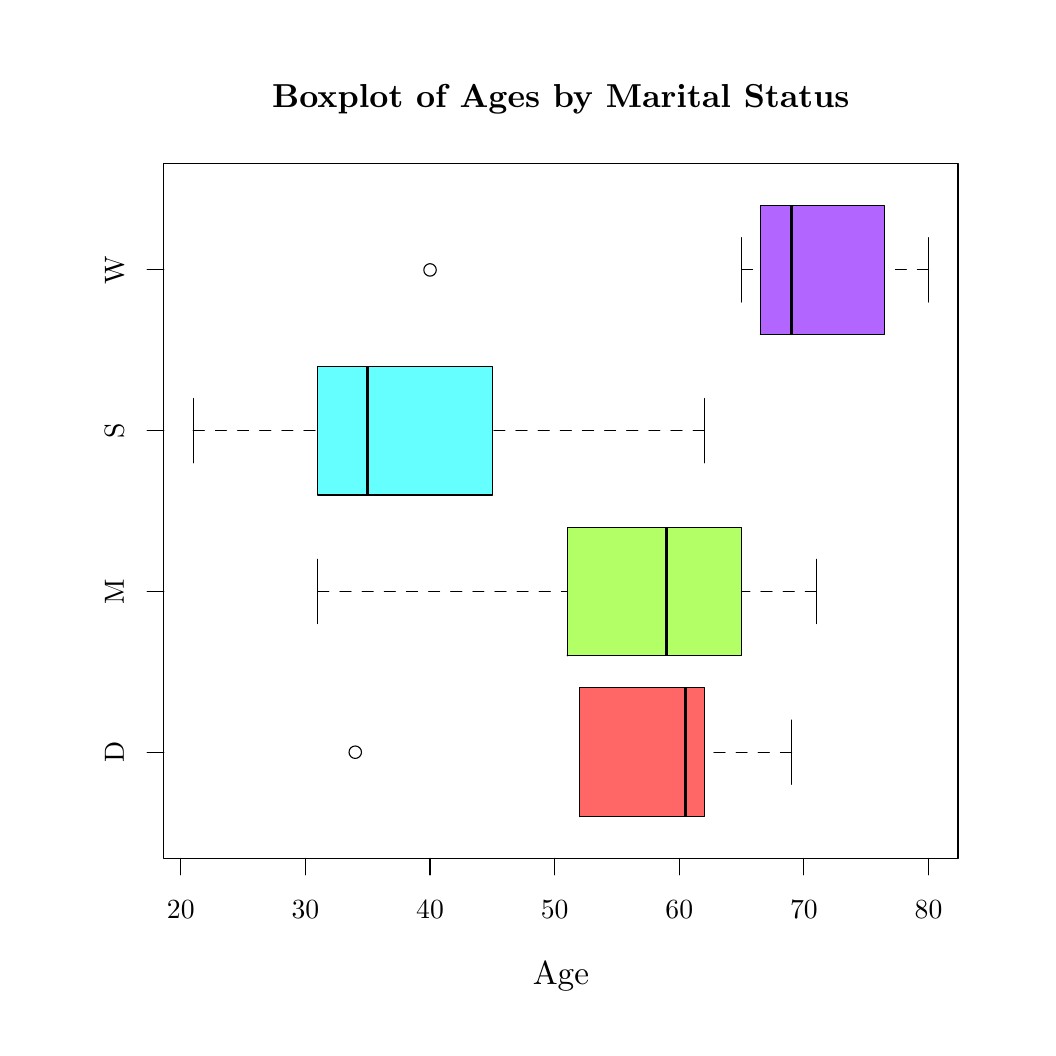
\begin{tikzpicture}[x=1pt,y=1pt]
\definecolor{fillColor}{RGB}{255,255,255}
\path[use as bounding box,fill=fillColor,fill opacity=0.00] (0,0) rectangle (361.35,361.35);
\begin{scope}
\path[clip] ( 49.20, 61.20) rectangle (336.15,312.15);
\definecolor{fillColor}{RGB}{255,102,102}

\path[fill=fillColor] (199.43, 76.30) --
	(199.43,122.78) --
	(244.46,122.78) --
	(244.46, 76.30) --
	cycle;
\definecolor{drawColor}{RGB}{0,0,0}

\path[draw=drawColor,line width= 1.2pt,line join=round] (237.71, 76.30) -- (237.71,122.78);

\path[draw=drawColor,line width= 0.4pt,dash pattern=on 4pt off 4pt ,line join=round,line cap=round] (199.43, 99.54) -- (199.43, 99.54);

\path[draw=drawColor,line width= 0.4pt,dash pattern=on 4pt off 4pt ,line join=round,line cap=round] (275.99, 99.54) -- (244.46, 99.54);

\path[draw=drawColor,line width= 0.4pt,line join=round,line cap=round] (199.43, 87.92) -- (199.43,111.16);

\path[draw=drawColor,line width= 0.4pt,line join=round,line cap=round] (275.99, 87.92) -- (275.99,111.16);

\path[draw=drawColor,line width= 0.4pt,line join=round,line cap=round] (199.43, 76.30) --
	(199.43,122.78) --
	(244.46,122.78) --
	(244.46, 76.30) --
	(199.43, 76.30);

\path[draw=drawColor,line width= 0.4pt,line join=round,line cap=round] (118.37, 99.54) circle (  2.25);
\definecolor{fillColor}{RGB}{179,255,102}

\path[fill=fillColor] (194.93,134.39) --
	(194.93,180.87) --
	(257.97,180.87) --
	(257.97,134.39) --
	cycle;

\path[draw=drawColor,line width= 1.2pt,line join=round] (230.95,134.39) -- (230.95,180.87);

\path[draw=drawColor,line width= 0.4pt,dash pattern=on 4pt off 4pt ,line join=round,line cap=round] (104.86,157.63) -- (194.93,157.63);

\path[draw=drawColor,line width= 0.4pt,dash pattern=on 4pt off 4pt ,line join=round,line cap=round] (284.99,157.63) -- (257.97,157.63);

\path[draw=drawColor,line width= 0.4pt,line join=round,line cap=round] (104.86,146.01) -- (104.86,169.25);

\path[draw=drawColor,line width= 0.4pt,line join=round,line cap=round] (284.99,146.01) -- (284.99,169.25);

\path[draw=drawColor,line width= 0.4pt,line join=round,line cap=round] (194.93,134.39) --
	(194.93,180.87) --
	(257.97,180.87) --
	(257.97,134.39) --
	(194.93,134.39);
\definecolor{fillColor}{RGB}{102,255,255}

\path[fill=fillColor] (104.86,192.48) --
	(104.86,238.96) --
	(167.91,238.96) --
	(167.91,192.48) --
	cycle;

\path[draw=drawColor,line width= 1.2pt,line join=round] (122.87,192.48) -- (122.87,238.96);

\path[draw=drawColor,line width= 0.4pt,dash pattern=on 4pt off 4pt ,line join=round,line cap=round] ( 59.83,215.72) -- (104.86,215.72);

\path[draw=drawColor,line width= 0.4pt,dash pattern=on 4pt off 4pt ,line join=round,line cap=round] (244.46,215.72) -- (167.91,215.72);

\path[draw=drawColor,line width= 0.4pt,line join=round,line cap=round] ( 59.83,204.10) -- ( 59.83,227.34);

\path[draw=drawColor,line width= 0.4pt,line join=round,line cap=round] (244.46,204.10) -- (244.46,227.34);

\path[draw=drawColor,line width= 0.4pt,line join=round,line cap=round] (104.86,192.48) --
	(104.86,238.96) --
	(167.91,238.96) --
	(167.91,192.48) --
	(104.86,192.48);
\definecolor{fillColor}{RGB}{179,102,255}

\path[fill=fillColor] (264.73,250.57) --
	(264.73,297.05) --
	(309.76,297.05) --
	(309.76,250.57) --
	cycle;

\path[draw=drawColor,line width= 1.2pt,line join=round] (275.99,250.57) -- (275.99,297.05);

\path[draw=drawColor,line width= 0.4pt,dash pattern=on 4pt off 4pt ,line join=round,line cap=round] (257.97,273.81) -- (264.73,273.81);

\path[draw=drawColor,line width= 0.4pt,dash pattern=on 4pt off 4pt ,line join=round,line cap=round] (325.52,273.81) -- (309.76,273.81);

\path[draw=drawColor,line width= 0.4pt,line join=round,line cap=round] (257.97,262.19) -- (257.97,285.43);

\path[draw=drawColor,line width= 0.4pt,line join=round,line cap=round] (325.52,262.19) -- (325.52,285.43);

\path[draw=drawColor,line width= 0.4pt,line join=round,line cap=round] (264.73,250.57) --
	(264.73,297.05) --
	(309.76,297.05) --
	(309.76,250.57) --
	(264.73,250.57);

\path[draw=drawColor,line width= 0.4pt,line join=round,line cap=round] (145.39,273.81) circle (  2.25);
\end{scope}
\begin{scope}
\path[clip] (  0.00,  0.00) rectangle (361.35,361.35);
\definecolor{drawColor}{RGB}{0,0,0}

\path[draw=drawColor,line width= 0.4pt,line join=round,line cap=round] ( 49.20, 99.54) -- ( 49.20,273.81);

\path[draw=drawColor,line width= 0.4pt,line join=round,line cap=round] ( 49.20, 99.54) -- ( 43.20, 99.54);

\path[draw=drawColor,line width= 0.4pt,line join=round,line cap=round] ( 49.20,157.63) -- ( 43.20,157.63);

\path[draw=drawColor,line width= 0.4pt,line join=round,line cap=round] ( 49.20,215.72) -- ( 43.20,215.72);

\path[draw=drawColor,line width= 0.4pt,line join=round,line cap=round] ( 49.20,273.81) -- ( 43.20,273.81);

\node[text=drawColor,rotate= 90.00,anchor=base,inner sep=0pt, outer sep=0pt, scale=  1.00] at ( 34.80, 99.54) {D};

\node[text=drawColor,rotate= 90.00,anchor=base,inner sep=0pt, outer sep=0pt, scale=  1.00] at ( 34.80,157.63) {M};

\node[text=drawColor,rotate= 90.00,anchor=base,inner sep=0pt, outer sep=0pt, scale=  1.00] at ( 34.80,215.72) {S};

\node[text=drawColor,rotate= 90.00,anchor=base,inner sep=0pt, outer sep=0pt, scale=  1.00] at ( 34.80,273.81) {W};

\path[draw=drawColor,line width= 0.4pt,line join=round,line cap=round] ( 55.32, 61.20) -- (325.52, 61.20);

\path[draw=drawColor,line width= 0.4pt,line join=round,line cap=round] ( 55.32, 61.20) -- ( 55.32, 55.20);

\path[draw=drawColor,line width= 0.4pt,line join=round,line cap=round] (100.36, 61.20) -- (100.36, 55.20);

\path[draw=drawColor,line width= 0.4pt,line join=round,line cap=round] (145.39, 61.20) -- (145.39, 55.20);

\path[draw=drawColor,line width= 0.4pt,line join=round,line cap=round] (190.42, 61.20) -- (190.42, 55.20);

\path[draw=drawColor,line width= 0.4pt,line join=round,line cap=round] (235.46, 61.20) -- (235.46, 55.20);

\path[draw=drawColor,line width= 0.4pt,line join=round,line cap=round] (280.49, 61.20) -- (280.49, 55.20);

\path[draw=drawColor,line width= 0.4pt,line join=round,line cap=round] (325.52, 61.20) -- (325.52, 55.20);

\node[text=drawColor,anchor=base,inner sep=0pt, outer sep=0pt, scale=  1.00] at ( 55.32, 39.60) {20};

\node[text=drawColor,anchor=base,inner sep=0pt, outer sep=0pt, scale=  1.00] at (100.36, 39.60) {30};

\node[text=drawColor,anchor=base,inner sep=0pt, outer sep=0pt, scale=  1.00] at (145.39, 39.60) {40};

\node[text=drawColor,anchor=base,inner sep=0pt, outer sep=0pt, scale=  1.00] at (190.42, 39.60) {50};

\node[text=drawColor,anchor=base,inner sep=0pt, outer sep=0pt, scale=  1.00] at (235.46, 39.60) {60};

\node[text=drawColor,anchor=base,inner sep=0pt, outer sep=0pt, scale=  1.00] at (280.49, 39.60) {70};

\node[text=drawColor,anchor=base,inner sep=0pt, outer sep=0pt, scale=  1.00] at (325.52, 39.60) {80};
\end{scope}
\begin{scope}
\path[clip] (  0.00,  0.00) rectangle (361.35,361.35);
\definecolor{drawColor}{RGB}{0,0,0}

\node[text=drawColor,anchor=base,inner sep=0pt, outer sep=0pt, scale=  1.20] at (192.68,332.61) {\bfseries Boxplot of Ages by Marital Status};

\node[text=drawColor,anchor=base,inner sep=0pt, outer sep=0pt, scale=  1.20] at (192.68, 15.60) {Age};
\end{scope}
\begin{scope}
\path[clip] (  0.00,  0.00) rectangle (361.35,361.35);
\definecolor{drawColor}{RGB}{0,0,0}

\path[draw=drawColor,line width= 0.4pt,line join=round,line cap=round] ( 49.20, 61.20) --
	(336.15, 61.20) --
	(336.15,312.15) --
	( 49.20,312.15) --
	( 49.20, 61.20);
\end{scope}
\end{tikzpicture}
}
\end{center}

\begin{enumerate}
\item Which group has higher ages?
\item Which group has lower central dispersion?
\item Which groups have outliers?
\item At which group is the age distribution more asymmetric?
\end{enumerate}
}
%SOLUTION
{
\begin{enumerate}
\item Widowers
\item Divorced.
\item Widowers and divorced.
\item Divorced.
\end{enumerate}
}
%RESOLUTION
{
}


\newproblem{des-60}{gen}{*}
%STATEMENT
{The systolic blood pressure (in mmHg) of a sample of persons is
\[
135\quad 128\quad 137\quad 110\quad 154\quad 142\quad 121\quad 127\quad 114\quad 103
\]

\begin{enumerate}
\item Calculate the central tendency statistics.
\item How is the relative dispersion with respect to the mean?
\item How is the skewness of the sample distribution?
\item How is the kurtosis of the sample distribution?
\item If we know that the method used for measuring the blood pressure is biased, and, in order to get the right values,
we have to apply the linear transformation $y=1.2x-5$, what are the statistics values of parts (a) to (d) for the new, corrected distribution?
\end{enumerate}


Use the following sums: $\sum x_i= 1271$ mmHg, $\sum (x_i-\bar x)^2=2188.9$ mmHg$^2$, $\sum (x_i-\bar x)^3=2764.32$
mmHg$^3$, $\sum (x_i-\bar x)^4=1040080$ mmHg$^4$.
}
%SOLUTION
{
Let $X$ be the systolic blood pressure.
\begin{enumerate}
\item $\bar{x}=127.1$ mmHg, $Me=127.5$ mmHg, $Mo$ all the values.
\item $s=14.7949$ mmHg and $cv=0.1164$.
\item $g_1=0.0854$, so the distribution is almost symmetric.
\item $g_2=-0.8292$, so the distribution is flatter than a normal distribution (platykurtic).
\item $\bar{y}=147.52$ mmHg, $Me=148$ mmHg, $Mo=157$ mmHg, $s=17.7539$ mmHg, $cv=0.1203$, $g_1=0.0854$ and $g_2=-0.8292$.
\end{enumerate}
}
%RESOLUTION
{
}

\newproblem{des-61}{gen}{*}
%STATEMENT
{The table below contains the frequency of pregnancies, abortions and births of a sample of 999 women in a city.

\begin{center}
\begin{tabular}{crrr}
\toprule
Num & Pregnancies & Abortions & Births\\
0 & 61 & 751 & 67 \\
1 & 64 & 183 & 80 \\
2 & 328 & 51 & 400 \\
3 & 301 & 10 & 300 \\
4 & 122 & 2 & 90 \\
5 & 81 & 2 & 62 \\
6 & 29 & 0 & 0 \\
7 & 11 & 0 & 0 \\
8 & 2 & 0 & 0 \\
\bottomrule
\end{tabular}
\end{center}

\begin{enumerate}
\item How many birth outliers are in the sample?
\item Which variable has lower spread with respect to the mean?
\item Which value is relatively higher, 7 pregnancies or 4 abortions? Justify your answer.
\end{enumerate}

Use the following sums:\\
Pregnancies: $\sum x_in_i= 2783$, $\sum x_i^2n_i=9773$.\\
Abortions: $\sum x_in_i= 333$, $\sum x_i^2n_i=559$.\\
Births: $\sum x_in_i= 2450$, $\sum x_i^2n_i=7370$.
}
%SOLUTION
{
Let $X$ be the number of pregnancies, $y$ to the number of abortions and $z$ to the number of births.
\begin{enumerate}
\item 129 outliers.
\item Pregnancies: $\bar{x}=2.7858$, $s_x=1.422$ and $cv_x=0.5105$.\\
Abortions: $\bar{y}=0.3333$, $s_y=0.6697$ and $cv_y=2.009$.
Births: $\bar{z}=2.4525$, $s_z=1.1674$ and $cv_z=0.476$.
\item The standard score of 7 pregnancies is $2.9635$, y de standard score of 4 abortions is $5.4754$, so 4 abortions is relatively greater than 7 pregnancies.
\end{enumerate}
}
%RESOLUTION
{
}

\newproblem{des-62}{far}{*}
%STATEMENT
{The gene of a rat species has been modified to help the metabolization of cholesterol in blood.
To check the effectiveness of this genetic modification two samples of 20 rats were drawn, ones with the gene modified and the others not, and they were fed with the same diet with different concentrations of palm oil during one month. 
The following sums summarize the results:

\textbf{Palm oil quantity in gr} (the same in both samples)\\
\(\sum x_i=640.6467\), \(\sum x_i^2=23508.6387\),
\(\sum(x_i-\bar x)^3=-5527.08\), \(\sum(x_i-\bar x)^4=792910\)\\
\textbf{Cholesterol level in blood in mg/dl of non genetically modified rats}\\
\(\sum y_j=2945.8545\), \(\sum y_j^2=439517.5975\),
\(\sum(y_j-\bar y)^3=604.08\), \(\sum(y_j-\bar y)^4=3717331.07\)\\
\textbf{Cholesterol level in blood in mg/dl of genetically modified rats}\\
\(\sum y_j=2126.5899\), \(\sum y_j^2=226824.5373\),
\(\sum(y_j-\bar y)^3=-629.4\), \(\sum(y_j-\bar y)^4=48248.29\)\\

\begin{enumerate}
\item In which sample the cholesterol has a more representative mean, genetically modified or non modified rats?
\item In which sample the distribution of cholesterol is more skew?
\item In which sample the kurtosis of the distribution of cholesterol is less normal?
\item Which rat has a cholesterol level relatively bigger, a genetically modified rat with a cholesterol level of 130 mg/dl, or a non genetically modified rat with a cholesterol level of 145 mg/dl?
\end{enumerate}
}
%SOLUTION
{\begin{enumerate}
\item Non genetically modified rats: $\bar y=147.2927$ mg/dl,  $s^2_y=280.7332$ (mg/dl)$^2$, $s=16.7551$ mg/dl and $cv_y=0.1138$.\\
Genetically modified rats: $\bar y=106.3295$ mg/dl,  $s^2_y=35.265$ (mg/dl)$^2$, $s=5.9384$ mg/dl and $cv_y=0.0558$.\\
Thus, the mean of genetically modified rats is more representative since the coef. of variation is smaller.
\item Non genetically modified rats: $g_1=0.0064$.\\
Genetically modified rats: $g_1-0.1503$.\\
Thus, the distribution of genetically modified rats is more skew since the coef. of skewness is further from 0.
\item Non genetically modified rats: $g_2=-0.6416$.\\
Genetically modified rats: $g_2-1.0602$.\\
Thus, the kurtosis of the distribution of genetically modified rats is less normal since the coef. of kurtosis is further from 0.
\item Non genetically modified rats: $z(145)=-0.1368$.\\
Genetically modified rats: $z(130)=3.986$.\\
Thus, a cholesterol level of 130 mg/dl in genetically modified rats is relatively greater than 145 mg/dl in non genetically modified rats.
\end{enumerate}
}
%RESOLUTION
{
}
% Author Alfredo Sánchez Alberca (asalber@ceu.es)

\newproblem{reg-1}{gen}{}
% ENUNCIADO
{Dada la siguiente tabla de correlación:
\begin{center}
\begin{tabular}{|c||c|c|c|}
\hline
$X\setminus Y$ & 1 & 2 & 3 \\ \hline\hline
$\left[ -2,2\right) $ & 3 & 6 & 1 \\ \hline
$\left[ 2,6\right) $ & 4 & 7 & 3 \\ \hline
$\left[ 6,10\right) $ & 5 & 3 & 0 \\ \hline
\end{tabular}
\end{center}

Determinar:
\begin{enumerate}
\item  Las distribuciones marginales. Media, Moda y Mediana.
\item  Rectas de Regresión.
\item  Coeficiente de correlación lineal. Interpretar el resultado.
\end{enumerate}
}
%SOLUTION
{}
%RESOLUTION
{}


\newproblem{reg-2}{med}{}
%STATEMENT
{Una compañía de asistencia sanitaria hace un estudio del número de veces que, durante el último trimestre, han acudido sus asegurados a consultas de especialistas, en función de su edad. En la siguiente tabla se reflejan los resultados obtenidos:
\begin{center}
\begin{tabular}{|c||c|c|c|c|c|}
\hline
$\mbox{Edad}\setminus \mbox{Cons.}$ & 0 & 1 & 2 & 3 & 4 \\ \hline\hline
$\left[ 30,40\right) $ & 6 & 2 & 2 & 0 & 0  \\ \hline
$\left[ 40,50\right) $ & 4 & 3 & 6 & 4 & 1 \\ \hline
$\left[ 50,60\right) $ & 0 & 2 & 4 & 5 & 3 \\ \hline
$\left[ 60,70\right) $ & 0 & 0 & 3 & 4 & 5 \\ \hline
$\left[ 70,80\right) $ & 0 & 0 & 0 & 4 & 6 \\ \hline
\end{tabular}
\end{center}

Se pide:
\begin{enumerate}
\item Recta de regresión del número de consultas sobre la edad.
\item Coeficiente de correlación e interpretarlo.
\item ¿Cuántas consultas se espera que realice una persona de 52 años?¿Es fiable esta predicción?
\end{enumerate}
}
%SOLUTION
{}
%RESOLUTION
{}


\newproblem{reg-3}{far}{}
%STATEMENT
{A research study has been conducted to determine the loss of activity of a drug.
The table below shows the results of the experiment.

\begin{center}
\begin{tabular}{|l|r|r|r|r|r|}
\hline
Time (in years) & 1 & 2 & 3 & 4 & 5 \\ \hline
Activity (\%) & 96 & 84 & 70 & 58 & 52 \\ \hline
\end{tabular}
\end{center}

\begin{enumerate}
\item  Construct the linear regression model of activity on time.
\item  According to the linear model, when will the activity be 80\%?
When will the drug have lost all activity?
Which prediction is more reliable?
Justify the answer.
\end{enumerate}
}
%SOLUTION
{Naming $T$ the time and $A$ the drug activity:
\begin{enumerate}
\item $\bar t=3$ years, $\bar a=72\%$, $s_t^2=2$ years$^2$, $s_a^2=264\%^2$, $s_{ta}=-22.8$ years$\cdot\%$.\\
Regression line of activity on time: $a=-11.4t+106.2$.
\item Regression line of time on activity: $t=-0.086a+9.2182$.\\
$t(80)=2.3091$ years and $t(0)=9.2182$ years.
\end{enumerate}
}
%RESOLUTION
{}


\newproblem{reg-4}{amb}{}
%STATEMENT
{Las temperaturas medias mensuales (en $^\circ$C) y las precipitaciones totales mensuales (en mm) durante el año 2001 en Madrid fueron:
\begin{center}
\begin{tabular}{|l|r|r|r|r|r|r|r|r|r|r|r|r|}
\cline{2-13}
\multicolumn{1}{c|}{} &    Ene &    Feb &    Mar &    Abr &    May &    Jun &    Jul &    Ago &    Sep &    Oct &    Nov &    Dic \\
\hline
Temp.               &  $7.2$ &  $8.4$ & $12.2$ & $13.7$ & $16.7$ & $23.3$ & $24.2$ & $25.5$ & $20.4$ & $16.2$ &  $8.1$ &  $4.2$ \\
\hline
Prec.                & $73.6$ & $31.7$ & $72.1$ & $20.7$ & $37.1$ & $3.8$ & $3.3$ & $1.5$ & $23.1$ & $67.0$ & $12.4$ & $18.0$ \\
\hline
\end{tabular}
\end{center}
¿Existe relación lineal entre las precipitaciones y la temperatura?
De acuerdo a esta relación, ¿qué cantidad de precipitaciones se espera que haya un mes con una temperatura media de 15$^\circ$C?¿Es fiable esta predicción?
}
%SOLUTION
{}
%RESOLUTION
{}


\newproblem{reg-5}{gen}{}
% ENUNCIADO
{Se ha realizado un estudio comparativo de las puntuaciones obtenidas por los alumnos en un test de ingreso en la
universidad ($X$), y el número de asignaturas aprobadas en el primer curso ($Y$). Los resultados obtenidos se expresan en
la siguiente tabla:

\begin{center}
\begin{tabular}{|c||c|c|c|c|c|}
\hline
$X\setminus Y$ & 0 & 1 & 2 & 3 & 4 \\ \hline\hline
$\left[ 0,10\right) $ & 2 & 2 & 1 & 0 & 0 \\ \hline
$\left[ 10,20\right) $ & 1 & 1 & 2 & 2 & 0 \\ \hline
$\left[ 20,30\right) $ & 0 & 1 & 3 & 4 & 1 \\ \hline
$\left[ 30,40\right) $ & 0 & 0 & 2 & 2 & 6 \\ \hline
\end{tabular}
\end{center}

Se desea calcular:
\begin{enumerate}
\item Recta de regresión de $X$ sobre $Y.$
\item Coeficiente de correlación e interpretación del mismo.
\item Si la universidad en cuestión sólo contara con alumnos que al menos logren aprobar dos asignaturas, ¿qué número
de preguntas respondidas correctamente exigirá en el test?
\end{enumerate}
}
%SOLUTION
{
\begin{enumerate}
\item $\bar x=23$ puntos, $\bar y=2.4$ asignaturas, $s_x^2=116$ puntos$^2$, $s_y^2=1.5733$ asignaturas$^2$,
$s_x=10.7703$ puntos, $s_y=1.2453$ asignaturas y $s_{xy}=9.8$ puntos$\cdot$asignaturas.\\
Recta de regresión de $X$ sobre $Y$: $x=6.2288y+8.0508$.
\item $r=0.73$, lo que quiere decir que hay buena relación lineal entre las puntuaciones y las asignaturas aprobadas y
además es creciente (a mayor puntuación en el test, más asignaturas aprobadas).
\end{enumerate}
}
%RESOLUTION
{}


\newproblem{reg-6}{nut}{*}
%STATEMENT
{The table below shows the two-dimensional frequency distribution of a sample of 80 persons in a study about the
relation between the blood cholesterol ($X$) in mg/dl and the high blood pressure ($Y$) in mmHg.
\[
\begin{array}{|c||c|c|c||c|}
\hline
X\setminus Y & [110,130) & [130,150) & [150,170) & n_x \\
\hline\hline
[170,190)   &           &     4     &           & 12\\
\hline
[190,210)   &    10     &    12     &     4     &   \\
\hline
[210,230)   &     7     &           &     8     &   \\
\hline
[230,250)   &     1     &           &           & 18\\
\hline\hline
n_y          &           &    30     &    24    &    \\
\hline
\end{array}
\]

\begin{enumerate}
\item Complete the table.
\item Construct the linear regression model of cholesterol on pressure.
\item Use the linear model to calculate the expected cholesterol for a person with pressure 160 mmHg.
\item According to the linear model, what is the expected pressure for a person with cholesterol 270 mg/dl?
\end{enumerate}

Use the following sums:
$\sum x_i=16960$ mg/dl, $\sum y_j=11160$ mmHg, $\sum x_i^2=3627200$ (mg/dl)$^2$, $\sum y_j^2=1576800$ mmHg$^2$ y
$\sum x_iy_j=2378800$ mg/dl$\cdot$mmHg.
}
%SOLUTION
{
\begin{enumerate}
\item Frequency table
\[
\begin{array}{|c||c|c|c||c|}
\hline
X\setminus Y & [110,130) & [130,150) & [150,170) & n_x \\
\hline\hline
[170,190)   &     8     &     4     &     0     & 12 \\
\hline
[190,210)   &    10     &    12     &     4     & 26 \\
\hline
[210,230)   &     7     &     9     &     8     & 24 \\
\hline
[230,250)   &     1     &     5     &    12     & 18 \\
\hline\hline
n_y          &   26     &    30     &    24     & 80 \\
\hline
\end{array}
\]
\item $\bar x=212$ mg/dl, $\bar y=139.5$ mmHg, $s_x^2=396$ (mg/dl)$^2$, $s_y^2=249.75$ mmHg$^2$ y $s_{xy}=161$
mg/dl$\cdot$mmHg. Regression line of cholesterol on pressure: $x=122.0721+0.6446y$.
\item  $x(160)=225.2152$ mg/dl.
\item Regression line of pressure on cholesterol: $y=0.4066x+53.3081$.\\
$y(270)=163.0808$ mmHg.
\end{enumerate}
}
%RESOLUTION
{}


\newproblem{reg-7}{nut}{*}
%STATEMENT
{A dietary center is testing a new diet in a sample of 12 persons.
The data below are the number of days of diet and the weight loss (in Kg) until them for every person.
\begin{center}
(33 , 3.9), (51 , 5.9), (30 , 3.2), (55 , 6.0), (38 , 4.9), (62 , 6.2),\\
(35 , 4.5), (60 , 6.1), (44 , 5.6), (69 , 6.2), (47 , 5.8), (40 , 5.3)
\end{center}
\begin{enumerate}
\item Draw the scatter plot. According to the point cloud, what type of regression model explains better the relation
between the weight loss and the days of diet?
\item Construct the linear regression model and the logarithmic regression model of the weight loss on the number of days of diet.
\item Use the best model to predict the weight that will lose a person after 40 and 100 days of diet.
Are these predictions reliable?
\end{enumerate}
Use the following sums ($X$=days of diet and $Y$=weight loss): $\sum x_i=564$ days, $\sum \log(x_i)=45.8086$
$\log(\mbox{days})$, $\sum y_j=63.6$ kg, $\sum x_i^2=28234$ days$^2$, $\sum \log(x_i)^2=175.6603$ $\log(\mbox{days})^2$, $\sum y_j^2=347.7$ kg$^2$, $\sum x_iy_j=3108.5$ days$\cdot$kg, $\sum \log(x_i)y_j=245.4738$ $\log(\mbox{days})\cdot$kg.
}
%SOLUTION
{Naming $Z=\log X$.
\begin{enumerate}[start=2]
\item $\bar x=47$ days, $\bar y=5.3$ kg, $s_x^2=143.833$ days$^2$, $s_y^2=0.885$ kg$^2$, $s_{xy}=9.942$ days$\cdot$kg.\\
Linear model: $y=0.069x+2.051$.\\
$\bar z=3.82$ $\log(\mbox{days})$, $s_z^2=0.07$ $\log^2(\mbox{days})$, $s_{yz}=0.22$ $\log(\mbox{days})\cdot\mbox{kg}$.\\
Logarithmic model: $y=3.4\log y-7.67$.
\item Linear model: $r^2=0.78$, logarithmic model: $r^2=0.86$.\\
Predictions with the logarithmic model: $y(40)=4.86$ kg and $y(100)=7.98$ kg.
The predictions are reliable since the coefficient of determination is high, although the prediction for 100 days is less reliable for being out of the range of observed values in the sample.
\end{enumerate}
}
%RESOLUTION
{}


\newproblem{reg-8a}{far}{*}
%STATEMENT
{In a study about the effect of different doses of a medicament, 2 patients got 2 mg and took 5 days to cure, 4
patients got 2 mg and took 6 days to cure, 2 patients got 3 mg ant took 3 days to cure, 4 patients got 3 mg and took 5
days to cure, 1 patient got 3 mg and took 6 days to cure, 5 patients got 4 mg and took 3 days to cure and 2 patients got
4 mg and took 5 days to cure.
\begin{enumerate}
\item Construct the joint frequency table.
\item Get the marginal frequency distributions and compute the main statistics for each variable.
\item Compute the covariance and interpret it.
\end{enumerate}
}
%SOLUTION
{Let $X$ be the dose and $Y$ to the curation time:
\begin{enumerate}[start=3]
\item $\bar x=3.05$ mg, $\bar y=4.55$ days, $s_x^2=0.648$ mg$^2$, $s_y^2=1.448$ days$^2$, $s_x=0.805$ mg, $s_y=1.203$
days and $s_{xy}=-0.678$ mg$\cdot$days, so there is a decreasing relation.
\end{enumerate}
}
%RESOLUTION
{}


\newproblem{reg-8b}{far}{*}
%STATEMENT
{Al realizar un estudio sobre la dosificación de un cierto medicamento, se trataron 6 pacientes con dosis diarias de 2
mg, 7 pacientes con 3 mg y otros 7 pacientes con 4 mg. De los pacientes tratados con 2 mg, 2 curaron al cabo de 5 días,
y 4 al cabo de 6 días. De los pacientes tratados con 3 mg diarios, 2 curaron al cabo de 3 días, 4 al cabo de 5 días y 1
al cabo de 6 días. Y de los pacientes tratados con 4 mg diarios, 5 curaron al cabo de 3 días y 2 al cabo de 5 días.

Se pide:
\begin{enumerate}
\item Dar el coeficiente de correlación e interpretación.
\item Determinar el tiempo esperado de curación para una dosis de 5 mg diarios.
\end{enumerate}
}
%SOLUTION
{Llamando $X$ a la dosis e $Y$ al tiempo de curación:
\begin{enumerate}
\item $\bar x=3.05$ mg, $\bar y=4.55$ días, $s_x^2=0.648$ mg$^2$, $s_y^2=1.448$ días$^2$, $s_x=0.805$ mg, $s_y=1.203$
días y $s_{xy}=-0.678$ mg$\cdot$días.\\
$r=-0.7$, que quiere decir que hay buena relación lineal entre la dosis y el tiempo de curación, y además es
decreciente (a mayor dosis, menor tiempo de curación).
\item Recta de regresión del tiempo de curación sobre la dosis: $y=-1.046x+7.741$.\\
$y(5)=2.511$ días.
\end{enumerate}
}
%RESOLUTION
{}


\newproblem{reg-9}{nut}{*}
%STATEMENT
{Después de tomar un litro de vino se ha medido la concentración de alcohol en la sangre en distintos instantes,
obteniendo:
\[
\begin{tabular}{|c|c|c|c|c|c|c|}
\hline
Tiempo después (minutos) & 30 & 60 & 90 & 120 & 150 & 180 \\ \hline
Concentración (gramos/litro) & 1.6 & 1.7 & 1.5 & 1.1 & 0.7 & 0.2 \\
\hline
\end{tabular}
\]

Se pide:
\begin{enumerate}
\item Calcular la recta de regresión de la concentración en función del tiempo.
\item ¿Qué concentración de alcohol habrá a los 100 minutos?
\item Si la concentración máxima de alcohol en la sangre que permite la ley para poder conducir es 0.8 g/l, ¿cuánto tiempo habrá que esperar después de tomarse un litro de vino para poder conducir sin infringir la ley?
\end{enumerate}
}
%SOLUTION
{}
%RESOLUTION
{}


\newproblem{reg-10}{gen}{}
%STATEMENT
{For two variables $X$ and $Y$ we have
\begin{itemize}
\item[--] The regression line of $Y$ on $X$ is $y-x-2=0$.
\item[--] The regression line of $X$ on $Y$ is $y-4x+22=0$.
\end{itemize}
Calculate:
\begin{enumerate}
\item The means $\bar x$ and $\bar y$.
\item The correlation coefficient.
\end{enumerate}
}
%SOLUTION
{
\begin{enumerate}
\item $\bar x=8$ and $\bar y=10$.
\item $r=0.5$.
\end{enumerate}
}
%RESOLUTION
{}


\newproblem{reg-11}{gen}{}
%STATEMENT
{The means of two variables $X$ and $Y$ are $\bar x=2$ and $\bar y=1$, and the correlation coefficient is 0.
\begin{enumerate}
\item  Predict the value of $Y$ for $x=10$.
\item  Predict the value of $X$ for $y=5$.
\item  Plot both regression lines.
\end{enumerate}
}
%SOLUTION
{
\begin{enumerate}
\item $y(10)=1$.
\item $x(5)=2$.
\end{enumerate}
}
%RESOLUTION
{}


\newproblem{reg-12}{gen}{*}
%STATEMENT
{En un estudio para relacionar la longitud de la línea de la vida de la mano izquierda y la duración de la vida de una
persona se han obtenido datos de 50 personas con los siguientes resultados ($X$=longitud de la línea en cm, $Y$=edad al
morir en años):
\[
\sum y=3333 \quad \sum y^2=231933 \quad \sum x=459.9 \quad \sum x^2=4308.57 \quad \sum xy=30949.
\]
A la vista de estos resultados, ¿cuanto vivirá, por termino medio, una persona con una línea de longitud 7.5 cm?
¿Es fiable esta estimación?  }
%SOLUTION
{$\bar x=9.198$ cm, $\bar y=66.66$ años, $s_x^2=1.568$ cm$^2$, $s_y^2=195.104$ años$^2$ y $s_{xy}=6.393$
cm$\cdot$años.\\
Recta de regresión de la edad al morir sobre la longitud de la línea de la vida: $y=4.077x+29.158$.\\
$y(7.5)=59.736$ años.\\
$r^2=0.13$, lo que quiere decir que casi no hay relación lineal entre las variables y la predicción anterior no es
fiable.}
%RESOLUTION
{}


\newproblem{reg-13}{gen}{*}
%STATEMENT
{En el estudio de regresión lineal con dos variables $X$ e $Y$ se sabe que $\overline{x}=30$, $\overline{y}=70$ y el
coeficiente de correlación lineal es $0.8$.
También se sabe que para $x=42$ el valor que predice la recta de regresión para $y$ es 78.

Se pide:
\begin{enumerate}
\item Calcular el valor de $x$ que se predice cuando $y=74$.
\item Explicar razonadamente en cuál de las dos variables es más representativa la media.
\end{enumerate}
}
%SOLUTION
{
\begin{enumerate}
\item Recta de regresión de $X$ sobre $Y$: $x=0.96x-37.2$.\\
$x(74)=33.84$.
\item $cv_x=0.0408\sqrt{s_{xy}}>cv_y=0.0146\sqrt{s_{xy}}$ y por tanto es más representativa la media de $Y$ pues tiene
menor dispersión relativa.
\end{enumerate}
}
%RESOLUTIONl
{}


\newproblem{reg-14}{gen}{*}
%STATEMENT
{The values of two variables $S$ and $T$ measured in 10 individuals are
\begin{center}
(-1.5, 2.25), (0.8, 0.64), (-0.2, 0.04), (-0.8, 0.64), (0.4, 0.16),\\
(0.2, 0.04), (-2.1, 4.41), (-0.4, 0.16), (1.5, 2.25), (2.1, 4.41).
\end{center}

\begin{enumerate}
\item Compute the covariance of $S$ and $T$.
\item Can we affirm that $S$ and $T$ are independent?
Justify the answer.
\item Use the regression line to predict the value of $S$ for $t=2$.
\end{enumerate}
}
%SOLUTION
{
\begin{enumerate}
\item $\bar s=0$, $\bar t=1.5$ and $s_{st}=0$.
\item We can affirm that there is no linear relationship between $S$ and $T$, but we can not affirm thar are independent.
\item $s(2)=0$.
\end{enumerate}
}
%RESOLUTION
{}


\newproblem{reg-15}{amb}{}
%STATEMENT
{En un experimento se ha medido el número de bacterias por unidad de volumen en un cultivo, cada hora transcurrida,
obteniendo los siguientes resultados:
\begin{center}
\begin{tabular}{c|ccccccccc}
Horas & 0 & 1 & 2 & 3 & 4 & 5 & 6 & 7 & 8  \\
\hline
Nº Bacterias & 25 & 28 & 47 & 65 & 86 & 121 & 190 & 290 & 362
\end{tabular}
\end{center}

Se pide:
\begin{enumerate}
\item Dibujar el diagrama de dispersión.
Según este diagrama, ¿qué tipo de modelo explicaría mejor la relación entre le número de bacterias y las horas
transcurridas?
\item Dibujar el diagrama de dispersión tomando una escala logarítmica para el número de bacterias.
\item Según el modelo anterior, ¿Cuántas bacterias tendríamos al cabo de 3 horas y media?
¿Y al cabo de 10 horas?
¿Son fiables estas predicciones?
\item ¿Cuánto tiempo tendría que transcurrir para que en el cultivo hubiese 100 bacterias?
\end{enumerate}
}
%SOLUTION
{Llamando $X$ a las horas, $Y$ a las bacterias y $Z$ al logaritmo neperiano de las bacterias:
\begin{enumerate}[start=3]
\item $\bar x=4$ horas, $\bar z=4.5149$ log(bacterias), $s_x^2=6.6667$ horas$^2$, $s_z^2=0.8361$ log$^2$(bacterias) y
$s_{xz}=2.3466$ horas$\cdot$log(bacterias).\\
Modelo lineal del logaritmo de las bacterias sobre las horas: $z=0.3520x+3.1070$.\\
Modelo exponencial de las bacterias sobre las horas: $y=e^{0.3520x+3.1070}$.\\
$y(3.5)=76.6254$ bacterias y $y(10)=755.0986$ bacterias.
\item Modelo lineal de las horas sobre el logaritmo de las bacterias: $x=2.8218z-8.7403$.\\
Modelo logarítmico de las horas sobre las bacterias: $x=2.8218\log y-8.7403$.\\
$x(100)=4.25$ horas.
\end{enumerate}
}
%RESOLUTION
{}


\newproblem{reg-16}{amb}{}
%STATEMENT
{Para evaluar la percepción de los ciudadanos sobre la contaminación atmosférica, se ha realizado un estudio en el que se ha medido en 12 ciudades la concentración media de CO (en mg/m$^3$ diarios), y la percepción mediana en la calidad el aire (en una muestra de individuos de tamaño fijo), medida en la escala MM=Muy Mala, M=Mala, A=Aceptable, B=Buena y MB=Muy Buena.
Los resultados obtenidos fueron:
\begin{center}
($12.8$ , A), ($11.6$ , A), ($9.8$ , B), ($10.3$ , MB), ($15.7$ , MM), ($18.2$ , M),\\
($11.8$ , B), ($16.7$ , M), ($14.5$ , M), ($12.1$ , A), ($19.4$ , MM), ($7.9$ , MB)
\end{center}
¿Existe relación entre la percepción de los habitantes de estas ciudades y la concentración de monóxido de carbono en la atmósfera de las mismas?
}
%SOLUTION
{}
%RESOLUTION
{}


\newproblem{reg-17}{med}{}
%STATEMENT
{En un estudio sobre la influencia del tabaco en los embarazos se ha medido en una muestra de 20 madres el número medio de cigarrillos diarios que fumaban las madres y el peso del recién nacido, obteniendo los siguientes resultados
\begin{center}
\begin{tabular}{|l|c|c|c|c|c|c|c|c|c|c|c|c|c|c|c|}
\hline
Cigarrillos &  2  &  3  & 10  &  8  & 12  &  6  &  6  &  5  &  4  &  9  & 14  &  3  &  7  & 8 &  2  \\
\hline
Peso (kg)  & 3.1 & 3.3 & 2.5 & 3.3 & 2.6 & 3.1 & 3.0 & 3.4 & 3.4 & 2.7 & 2.5 & 3.7 & 3.1 & 3 & 3.6 \\
\hline
\end{tabular}
\end{center}

Se pide:
\begin{enumerate}
\item Construir el modelo de regresión logarítmico del peso sobre el número de cigarrillos.
\item Según este modelo, ¿cuanto pesará el recién nacido si la madre fumaba 15 cigarrillos diários?
Es fiable esta predicción.
\item ¿Es mejor el modelo lineal a la hora de hacer predicciones?
\end{enumerate}
}
%SOLUTION
{}
%RESOLUTION
{}


\newproblem{reg-18}{med}{*}
%STATEMENT
{The table below contains the age in years and the systolic pressure in mmHg of 15 individuals.
\[
\begin{array}{|c|c|c|c|c|c|}
\hline
\text{Age} (x) & 20 & 30 & 40 & 50 & 60 \\
\hline
& 121 & 131 & 132 & 136 & 134\\
\text{Systolic pressure} (y) & 130 & 125 & 129 & 128 & 142 \\
& 125 & 128 & 131 & 134 & 137\\
\hline
\end{array}
\]

\begin{enumerate}
\item What percentage of the systolic pressure variance is explained by the age according to the linear regression model?
\item According to that regression model, what age corresponds to an individual with a systolic pressure of 133 mmHg.
Is reliable this prediction? 
Justify the answer. 
\end{enumerate}
Use the following sums for the computations:
$\sum x_i=600$ years, $\sum y_j=1963$ mmHg, $\sum x_i^2=27000$ years$^2$, $\sum y_j^2=257287$ mmHg$^2$ and $\sum x_iy_j=79400$ years$\cdot$mmHg.
}
%SOLUTION
{
\begin{enumerate}
\item $\bar x=40$ years, $\bar y=130.867$ mmHg, $s_x^2=200$ years$^2$, $s_y^2=26.295$ mmHg$^2$ y $s_{xy}=58.667$
years$\cdot$mmHg.\\
$r^2=0.654$, thus $65.4\%$ of the systolic pressure variance is explained by the age according to the linear regression model.
\item Regression line of age on systolic pressure: $x=2.231y-251.978$.\\
$x(133)=44.745$ years. This prediction is moderately reliable since the determination coefficient is moderately high. 
\end{enumerate}
}
%RESOLUTION
{}


\newproblem{reg-19}{qui}{*}
%STATEMENT
{Se ha realizado un estudio de regresión para ver la relación que existe entre la velocidad de transformación de una determinada sustancia química en una reacción y la temperatura a la que se realiza dicha reacción (manteniendo las cantidades de reactivos constantes).
Según una recta de regresión, a 10 ºC le correspondería una velocidad de 5 gr/min, y a 30 ºC le correspondería una velocidad de 15 gr/min.
Y según la otra recta, a una velocidad de 8 gr/min le correspondería una temperatura de 17 ºC, y a una velocidad de 16 gr/min le correspondería una temperatura de \mbox{31 ºC}. Se pide:
\begin{enumerate}
\item Calcular las ecuaciones de las rectas de regresión.
\item Calcular las medias de ambas variables.
\item Calcular el coeficiente de determinación. ¿Podemos decir que las predicciones del enunciado son fiables? Justificar la respuesta.
\end{enumerate}
}
%SOLUTION
{}
%RESOLUTION
{}


\newproblem{reg-20}{amb}{*}
%STATEMENT
{En un estudio ambiental de una comunidad autónoma se afirma que el número de hectáreas quemadas en los últimos 6 años está relacionado con la cantidad de precipitación media caída en la comunidad, en litros por metro cuadrado. Los datos que han manejado son:
\begin{center}
\begin{tabular}{|l|l|l|}
\hline
\multicolumn{1}{|c|}{Año} & \multicolumn{1}{c|}{Hectáreas quemadas} & \multicolumn{1}{c|}{Precipitación (l/m$^2$)} \\
\hline
\multicolumn{1}{|c|}{2000} & \multicolumn{1}{c|}{1250} & \multicolumn{1}{c|}{420} \\
\hline
\multicolumn{1}{|c|}{2001} & \multicolumn{1}{c|}{1400} & \multicolumn{1}{c|}{380} \\
\hline
\multicolumn{1}{|c|}{2002} & \multicolumn{1}{c|}{850} & \multicolumn{1}{c|}{460} \\
\hline
\multicolumn{1}{|c|}{2003} & \multicolumn{1}{c|}{1650} & \multicolumn{1}{c|}{370} \\
\hline
\multicolumn{1}{|c|}{2004} & \multicolumn{1}{c|}{900} & \multicolumn{1}{c|}{410} \\
\hline
\multicolumn{1}{|c|}{2005} & \multicolumn{1}{c|}{1700} & \multicolumn{1}{c|}{310} \\
\hline
\end{tabular}
\end{center}

\begin{enumerate}
\item Calcular la recta de regresión del número de hectáreas quemadas en función de la precipitación media anual.
\item ¿Es el modelo lineal un buen modelo de ajuste para la nube de puntos? Justificar la respuesta.
\end{enumerate}
}
%SOLUTION
{}
%RESOLUTION
{}


\newproblem{reg-21}{far}{}
%STATEMENT
{Se desea comprobar si el número de ventas de un fármaco depende del descuento que se aplique sobre él.
Para ello se ha medido el número de ventas en farmacias que aplican distintos descuentos obteniendo la siguiente muestra:
\begin{center}
\begin{tabular}{|c||c|c|c|c|c|c|c|c|c|c|c|c|c|c|}
\hline Descuento (\%) & 20 & 16 & 15 & 10 & 12 & 11 & 16 & 8 & 18 & 12 & 12 & 10 & 15 & 14 \\
\hline Ventas & 98 & 46 & 40 & 15 & 21 & 19 & 50 & 8 & 71 & 24 & 21 & 16 & 39 & 32 \\
\hline
\end{tabular}
\end{center}
Se pide:
\begin{enumerate}
\item Construir los modelos exponencial y logarítmico.
\item ¿Cuál de ellos expresa mejor la relación entre el descuento y las ventas?
\item ¿Qué descuento tendremos que aplicar si queremos vender al menos 50 fármacos?
\end{enumerate}
}
%SOLUTION
{}
%RESOLUTION
{}


\newproblem{reg-22}{amb}{*}
% ENUNCIADO
{Para ver si un aditivo para la gasolina mejora la combustión aumentando la emisión de dióxido de carbono, se ha hecho un
estudio en el que se ha medido la cantidad de aditivo añadida a cada litro de gasolina y el porcentaje de CO$_2$ emitido
por un mismo motor, obteniendo la siguiente muestra: \[
\begin{array}{|l|rrrrrrrr|}
\hline
\mbox{Aditivo (cl/l)} &  0.2 &  0.4 &  0.6 &  0.8 &  1.0 &  1.2 &  1.4 &  1.6 \\
\hline
\mbox{CO$_2$ (\%)}         & 11.2 & 12.0 & 12.7 & 13.3 & 13.5 & 13.7 & 13.8 & 13.9 \\
\hline
\end{array}
\]
Se pide:
\begin{enumerate}
\item Calcular el modelo de regresión lineal y logarítmico del CO$_2$ sobre el aditivo.
¿Cuál de los dos modelos es mejor?
\item Según el mejor de los modelos anteriores, ¿cuánto CO$_2$ se producirá para $0.5$ cl de aditivo? ¿y para 2 cl?
¿Son fiables estas predicciones?
\item La normativa sobre emisión de gases exige que el porcentaje mínimo de CO$_2$ en la combustión debe superar al menos el $12.5\%$.
¿Cuánto aditivo es necesario para garantizar esto?
\end{enumerate}
}
%SOLUTION
{}
%RESOLUTION
{}


\newproblem{reg-23}{amb}{*}
%STATEMENT
{La siguiente tabla muestra los datos de emisiones de CO$_2$ y CH$_4$ (en kg/hab) y el producto interior bruto per cápita (en miles US\$) de varios países en el último año:
\[
\begin{array}{|l|r|r|r|}
\hline
\mbox{País} & \mbox{CO}_2 & \mbox{CH}_4 & \mbox{PIB}\\
\hline\hline
\mbox{Austria}     & 7.60 & 0.97 & 38.40\\ \hline
\mbox{España}      & 6.73 & 0.81	& 30.12\\ \hline
\mbox{Francia}     & 5.71 & 0.94	& 33.19\\ \hline
\mbox{EEUU}        &19.40 & 1.72	&	45.84\\ \hline
\mbox{Alemania}    & 9.80 & 0.83	& 34.18\\ \hline
\mbox{Canadá}      &15.60 & 3.08	& 38.43\\ \hline
\mbox{Italia}      & 7.29 & 0.58	& 30.44\\ \hline
\mbox{Japón}       &	9.44 & 0.16	& 33.58\\ \hline
\mbox{Australia}   &17.48 & 6.36	& 36.26\\ \hline
\mbox{Reino Unido} & 8.99 & 0.76	& 35.13\\ \hline
\end{array}
\qquad
\begin{array}{|l|r|r|r|}
\hline
\mbox{País} & \mbox{CO}_2 & \mbox{CH}_4 & \mbox{PIB}\\
\hline\hline
\mbox{Bolivia}     & 1.05 & 3.44	& 40.13\\ \hline
\mbox{Niger}       &	0.1	 & 0.12	&	 0.67\\ \hline
\mbox{Senegal}     &	0.35 & 0.76 &  1.69\\ \hline
\mbox{Pakistán}    & 0.65 & 0.59	&  2.59\\ \hline
\mbox{Filipinas}   &	0.83 & 0.46	&  3.38\\ \hline
\mbox{Perú}        & 0.94 & 0.75	&  7.80\\ \hline
\mbox{Túnez}      & 2.17 & 0.48	&  7.47\\ \hline
\mbox{Nepal}       & 0.13 & 0.90	&  1.21\\ \hline
\mbox{Nicaragua}   & 0.7	 & 0.32	&  2.62\\ \hline
\mbox{Mauritania}  & 0.97 & 0.85	&  2.01\\ \hline
\end{array}
\]
Utilizando los datos sin agrupar, calcular el modelo de regresión logarítmico que explique las emisiones de CO$_2$ en función del PIB y utilizarlo para predecir las emisiones de un país con 10 mil US\$ de PIB.
¿Es fiable la predicción?
}
%SOLUTION
{}
%RESOLUTION
{}


\newproblem{reg-24}{med}{*}
%STATEMENT
{A blood bank keeps plasma at a temperature of 0ºF.
When it is required for a blood transfusion, it is heated in an oven at a constant temperature of 120ºF.
In an experiment it has been measured the temperature of plasma at different times during the heating.
The results are in the table below.
\begin{center}
\begin{tabular}{lrrrrrrrr}
\toprule
Time (min)	& 5 & 8 & 15 & 25 & 30 & 37 & 45 & 60\\
Temperature (ºF) & 25 & 50 & 86 & 102 & 110 & 114 & 118 & 120\\
\bottomrule
\end{tabular}
\end{center}
\begin{enumerate}
\item Plot the scatter plot.
Which type of regression model do you think explains better relationship between temperature and time?
\item Which transformation should we apply to the variables to have a linear relationship?
\item Compute the logarithmic regression of the temperature on time.
\item According to the logarithmic model, what will the temperature of the plasma be after 15 minutes of heating?
Is this prediction reliable? Justify your answer.
\end{enumerate}

Use the following sums ($X$=Time and $Y$=Temperature): $\sum x_i=225$ min, $\sum \log(x_i)=24.5289$ $\log(\mbox{min})$, $\sum y_j=725$ ºF, $\sum \log(y_j)=35.2051$ $\log(\mbox{ºF})$, $\sum x_i^2=8833$ min$^2$, $\sum \log(x_i)^2=80.4703$ $\log(\mbox{min})^2$, $\sum y_j^2=74345$ ºF$^2$, $\sum \log(y_j)^2=157.1023$ $\log(\mbox{ºF})^2$, $\sum x_iy_j=24393$ min$\cdot$ºF, $\sum x_i\log(y_j)=1048.0142$ min$\cdot \log(\mbox{ºF})$, $\sum \log(x_i)y_j=2431.7096$ $\log(\mbox{min})$ºF, $\sum \log(x_i)\log(y_j)=111.1165$ $\log(\mbox{min})\log(\mbox{ºF})$.
}
%SOLUTION
{
\begin{enumerate}
\item A logarithmic model.
\item Apply a logarithmic transformation to time, $z=\log(x)$.
\item $\bar z=3.0661$ $\log(\mbox{min})$, $s_z^2=0.6577$ $\log^2(\mbox{min})$, $\bar y=90.625$ ºF, $s_y^2=1080.2344$ ºF$^2$ and $s_{zy}=26.0969$ $\log(\mbox{min})$ºF.\\
Logarithmic model of temperature on time: $y=-31.0325+39.6781\log(x)$.
\item $y(15)=76.4176$ ºF. $r^2=0.9586$, that is close to 1, so the prediction is reliable.
\end{enumerate}
}
%RESOLUTION
{}


\newproblem{reg-25}{far}{*}
%STATEMENT
{The concentration of a drug in blood, in mg/dl, depends on time, in hours, according to the data below.
\begin{center}
\begin{tabular}{lrrrrrrr}
\toprule
Time & 2 & 3 & 4 & 5 & 6 & 7 & 8\\
Drug concentration & 25 & 36 & 48 & 64 & 86 & 114 & 168\\
\bottomrule
\end{tabular}
\end{center}
\begin{enumerate}
\item Construct the linear regression model of drug concentration on time.
\item Construct the exponential regression model of drug concentration on time.
\item Use the best regression model to predict the drug concentration after $4.8$ hours? Is this prediction reliable?
\end{enumerate}

Use the following sums ($C$=Drug concentration and $T$=time): $\sum t_i=35$ h, $\sum \log(t_i)=10.6046$
$\log(\mbox{h})$, $\sum c_j=541$ mg/dl, $\sum \log(c_j)= 29.147$ $\log(\mbox{mg/dl})$, $\sum t_i^2=203$ h$^2$,
$\sum \log(t_i)^2=17.5206$ $\log(\mbox{h})^2$, $\sum c_j^2=56937$ (mg/dl)$^2$, $\sum \log(c_j)^2=124.0131$
$\log(\mbox{mg/dl})^2$, $\sum t_ic_j=3328$ h$\cdot$mg/dl, $\sum t_i\log(c_j)=154.3387$
h$\cdot\log(\mbox{mg/dl})$, $\sum \log(t_i)c_j=951.6961$ $\log(\mbox{h})\cdot$mg/dl, $\sum
\log(t_i)\log(c_j)=46.08046$ $\log(\mbox{h})\cdot\log(\mbox{mg/dl})$.
}
%SOLUTION
{Naming $Z=\log(C)$.
\begin{enumerate}
\item $\bar t=5$ hours, $\bar c=77.2857$ mg/dl, $s_t^2=4$ hours$^2$,  $s_c^2=2160.7755$ (mg/dl)$^2$, $s_{tc}=89$ hours(mg/dl).\\
Linear model of $C$ on $T$: $c=-33.9643+22.25t$.\\
$r^2=0.9165$.
\item  $\bar z=4.1639$ $\log$(mg/dl), $s_z^2=0.3785$ $\log^2$(mg/dl),
$s_{tz}=1.2291$ hours$\cdot\log$(mg/dl).\\
Exponential model of $C$ on $T$: $c=e^{0.3073t+2.6275}$.\\
$r^2=0.9979$.
\item $c(4.8)= 60.498$ mg/dl and is quite reliable since the coefficient of determination is close to 1.
\end{enumerate}
}
%RESOLUTION
{En el primer apartado de este problema debemos trabajar con el modelo exponencial de la concentración en función del
tiempo, por lo que vamos a tener que calcular la recta de regresión de $z=\ln C$ en función de $t$. Además, en el
segundo apartado debemos trabajar con el modelo lineal de $t$ en función de $C$. Por lo tanto, la tabla con los
sumatorios precisos es:
\[
\begin{array}{|l|r|r|r|r|r|r|r|}
\hline
t_i & c_i & t_i^2 & c_i^2 & t_i \cdot c_i & z_i=\ln_i & z_i^2 & t_i \cdot z_i \\
\hline
2 & 25 & 4 & 625 & 50 & 3.219 & 10.362 & 6.438 \\
\hline
3 & 36 & 9 & 1296 & 108 & 3.584 & 12.845 & 10.752 \\
\hline
4 & 48 & 16 & 2304 & 192 & 3.871 & 14.985 & 15.484 \\
\hline
5 & 64 & 25 & 4096 & 320 & 4.159 & 17.297 & 20.795 \\
\hline
6 & 86 & 36 & 7396 & 516 & 4.454 & 19.838 & 26.724 \\
\hline
7 & 114 & 49 & 12996 & 798 & 4.736 & 22.430 & 33.152 \\
\hline
8 & 168 & 64 & 28224 & 1344 & 5.124 & 26.255 & 40.992 \\
\hline
\sum= 35 & 541 & 203 & 56937 & 3328 & 29.147 & 124.012 & 154.337 \\
\hline
\end{array}
\]

\begin{enumerate}
\item Para el modelo exponencial de la concentración en función del tiempo tenemos en cuenta que:
\[
C = a \cdot e^{bt}  \Leftrightarrow \ln C = \ln \left( {a \cdot e^{bt} } \right) = \ln a + bt
\]
Por lo tanto, si $z=\ln C$, entonces:
\[
z=\ln a +bt
\]
Y el modelo exponencial se transforma en un modelo lineal de $z$ en función de $t$.

Por otra parte, sabemos que la recta de regresión de $z$ en función de $t$ viene dada por:
\[
z-\bar z = \frac{s_{tz}}{s_t^2}(t-\bar t)
\]
Y teniendo en cuenta los sumatorios obtenidos:
\begin{align*}
\bar t &= \frac{\sum t_i}{n} = \frac{35}{7} = 5,\\
\bar z &= \frac{\sum z_i}{n} = \frac{29.147}{7} = 4.164,\\
s_t ^2  &= \frac{\sum t_i^2}{n}-\bar t^2 = \frac{203}{7}-5^2 = 4,\\
s_z ^2  &= \frac{\sum z_i^2}{n}-\bar z^2 = \frac{124.012}{7}-4.164^2 = 0.38,\\
s_{tz}  &= \frac{\sum t_i z_i}{n}-\bar t \cdot \bar z = \frac{154.337}{7}-5 \cdot 4.164 = 1.228.
\end{align*}

Donde la media de $t$ viene dada en horas, su varianza en horas al cuadrado, la media de $z$ no tiene unidades ($z$ es
un logaritmo neperiano), tampoco las tiene su varianza, y la covarianza tiene las unidades de $t$, es decir horas.

Con todo ello, la ecuación de la recta de regresión de $z$ en función $t$ vale:
\[
z-4.164 = \frac{1.228}{4}(t-5)\Leftrightarrow z=2.629+0.307\cdot t
\]

Por lo tanto, teniendo en cuenta que:
\[
z=\ln a +b \cdot t=2.629+0.307 \cdot t
\]
obtenemos fácilmente que $b= 0.307$, y para $a$ despejamos tomando exponenciales:
\[
\ln a= 2.629\Leftrightarrow a=e^{2.629} =13.860.
\]
Con todo ello, cuando $t_0=4.8$ horas, el valor obtenido para $C_0$ (en mg/dl) vale:
\[
C(4.8)=13.860 e^{0.307 \cdot 4.8}=60.498 \text{ mg/dl}.
\]

Para ver si es fiable o no la predicción, calculamos el coeficiente de determinación (o el coeficiente de correlación):
\[
r^2  = \frac{{s_{tz} ^2 }}{{s_t ^2 s_z ^2 }} = \frac{{1.228^2 }}{{4 \cdot 0.377}} = 0.999,
\]
luego, mediante el modelo exponencial estamos explicando un $99.9\%$ de la variabilidad de la nube de puntos, y el
modelo exponencial es muy bueno. Por lo tanto, si el modelo es muy bueno y además la predicción la realizamos en
$t_0=4.8$, que está dentro del rango en el que hemos calculado el modelo, sin duda la predicción también será muy
fiable.

\item Para este nuevo apartado debemos predecir el tiempo que debe transcurrir para que la concentración sea de 100
mg/dl mediante un modelo lineal. Por lo tanto necesitamos la recta de regresión del tiempo en función de la concentración:
\[
t-\bar t = \frac{s_{tC}}{s_C^2}(C-\bar C)
\]
Mediante los sumatorios obtenidos en la tabla del comienzo, calculamos:
\begin{align*}
\bar C &= \frac{\sum C_i}{n} = \frac{541}{7} = 77.286,\\
s_C ^2 &= \frac{\sum z_i ^2}{n}-\bar z^2 = \frac{56937}{7}-77.286^2 = 2160.731,\\
s_{tC} &= \frac{\sum t_i C_i}{n}-\bar t \cdot \bar C = \frac{3328}{7}-5 \cdot 77.286 = 90.000.
\end{align*}
Donde la media de $C$ viene dada en mg/dl, su varianza en (mg/dl)$^2$, y la covarianza en horas$\cdot$(mg/dl).

Sustituyendo todo en la ecuación de la recta obtenemos:
\[
t-5 = \frac{90.000}{2160.731}(C-77.286)\Leftrightarrow t=0.0417 \cdot C+ 1.781
\]

Por lo tanto, si $C_0= 100$ entonces $t_0=5.951$ horas.
Para ver si la predicción es adecuada, de nuevo calculamos el coeficiente de determinación:
\[
r^2 = \frac{s_{tC}^2}{s_t ^2 s_C ^2} = \frac{90.000^2}{4 \cdot 2160.731} = 0.937.
\]
Lo cual nos confirma que el modelo lineal, aunque peor que el exponencial, sigue siendo un muy buen modelo.
Si a eso unimos que estamos realizando la predicción dentro del rango de concentraciones en las que lo hemos calculado,
concluimos que sí que será fiable.
\end{enumerate}
}


\newproblem{reg-26}{fis}{}
%STATEMENT
{The activity of a radioactive substance depends on time according to the data in the table below.
\[
\begin{array}{lrrrrrrrr}
\toprule
t\mbox{ (hours)} & 0 & 10 & 20 & 30 & 40 & 50 & 60 & 70 \\
A\mbox{ ($10^7$ disintegrations/s)} & 25.9 & 8.16 & 2.57 & 0.81 & 0.25 & 0.08 & 0.03 & 0.01\\
\bottomrule
\end{array}
\]

\begin{enumerate}
\item Represent graphically the data of radioactivity as a function of time.
Which type of regression model explains better the relationship between radioactivity and time?
\item Represent graphically the data of radioactivity as a function of time in a semi-logarithmic paper.
\item Compute the regression line of the logarithm of radioactivity on time.
\item Taking into account that radioactivity decay follows the formula
\[
A(t) = A_0 e^{-\lambda t}
\]
where $A_0$ is the number of disintegrations at the beginning and $\lambda$ is a disintegration constant, different for each radioactive substance, use the slope of the previous regression line to compute the disintegration constant for the substance.
\end{enumerate}
Use the following sums ($X$=Time and $Y$=Radioactivity): $\sum x_i=280$ hours, $\sum y_j=37.81$ $10^7$ disintegrations/s, $\sum \log(y_j)=-5.9371$  $\log(10^7 \mbox{ disintegrations/s})$, $\sum x_i^2=14000$ hours$^2$, $\sum y_j^2=744.7265$ $(10^7$ disintegrations/s$)^2$, $\sum \log(y_j)^2=57.7369$  $\log(10^7 \mbox{ disintegrations/s})^2$, $\sum x_iy_j=173.8$ hours$\cdot 10^7$ disintegrations/s, $\sum x_i\log(y_j)=-680.9447$ hours$\cdot \log(10^7 \mbox{disintegrations/s})$.
}
%SOLUTION
{Naming $Z=\log(Y)$.
\begin{enumerate}[start=3]
\item $\bar x=35$ hours, $\bar z=-0.7421$ $10^7$ disintegrations/s, $s_x^2=525$ hours$^2$, $s_z^2=6.6664$ $(10^7$ disintegrations/s$)^2$ and $s_{xz}=-59.1434$ hours$\cdot 10^7$ disintegrations/s.\\
Regression line of the logarithm of radioactivity on time: $z=-0.1127x+3.2008$.
\item $\lambda=0.1127$.
\end{enumerate}
}
%RESOLUTION
{}


\newproblem{reg-27}{qui}{}
%STATEMENT
{For oscillations of small amplitude, the oscillation period $T$ of a pendulum is given by the formula
\[
T = 2\pi\sqrt{\frac{L}{g}}
\]
where $L$ is the length of the pendulum and $g$ is the gravitational constant.
In order to check if the previous formula is satisfied, an experiment has been conducted where it has been measured the oscillation period for different lengths of the pendulum.
The measurements are shown in the table below.

\[
\begin{array}{lrrrrr}
\toprule
L\text{ (cm)} & 52.5 & 68.0 & 99.0 & 116.0 & 146.0 \\
P\text{ (seg)} & 1.449 & 1.639 & 1.999 & 2.153 & 2.408\\
\bottomrule
\end{array}
\]

\begin{enumerate}
\item Represent graphically the data of the period versus the length of the pendulum.
Does a linear model fit well to the points cloud?
\item Represent graphically the data of the period versus the length in a logarithmic paper.
Which type of model fits better to the points cloud?
\item Compute the regression line of the logarithm of period on the logarithm of length.
\item Taking in to account the independent term of the previous regression line, compute the value of $g$.
\end{enumerate}
}
%SOLUTION
{Let $X$ be the logarithm of length and $Y$ to the logarithm of period.
\begin{enumerate}[start=3]
\item $\bar x=4.5025$ $\log$(cm), $\bar y=0.6407$ $\log$(s), $s_x^2=0.1353$ $\log^2$(cm), $s_y^2=0.0339$ $\log^2$(s), $s_{xy}=0.0677$ $\log(\mbox{cm})\log(\mbox{s})$.\\
Regression line of $Y$ on $X$: $y=0.5006x-1.6132$.
\item $g=994.4579$ cm/s$^2$.
\end{enumerate}
}
%RESOLUTION
{}


\newproblem{reg-28}{far}{}
%STATEMENT
{En análisis colorimétrico, es frecuente utilizar la fracción de luz que absorbe una determinada sustancia disuelta
como una medida de la concentración con la que dicha sustancia está presente en la disolución, siempre y cuando se
utilice luz monocromática y la misma longitud recorrida por la luz en cada una de las mediciones.
Si llamamos $I_0$ a la intensidad de luz incidente, $I$ a la intensidad de luz transmitida y $C$ a la concentración de
la sustancia analizada, en un experimento de análisis colorimétrico realizado con Mn y una longitud de onda de 525 nm,
se han obtenido los siguientes datos, donde la concentración de Mn viene dada en mg por cada 100 ml de disolución:
\[
\begin{array}{|l|r|r|r|r|}
\hline
C & 1.00 & 2.00 & 3.00 & 4.00\\
\hline
I/I_0 & 0.418 & 0.149 & 0.058 & 0.026\\
\hline
\end{array}
\]

Se pide:
\begin{enumerate}
\item Representar los datos considerando $I/I_0$ en función de función de $C$.
A la vista de la nube de puntos, ¿qué modelo de regresión sería el más adecuado para expresar la relación entre las
variables?
\item Representar los datos pero en papel semilogarítmico.
\item Calcular la ecuación de la recta de regresión del logaritmo neperiano de $I/I_0$ frente a $C$.
\end{enumerate}
}
%SOLUTION
{Llamando $C$ a la concentración e $Z$ al logaritmo neperiano de $I/I_0$.
\begin{enumerate}[start=3]
\item $\bar c=2.5$ mg/100ml, $\bar z=-2.3183$, $s_c^2=1.25$ (mg/100ml)$^2$, $s_z^2=1.0788$ y $s_{cz}=-1.1595$.\\
Recta de regresión de $Z$ sobre $C$: $z=-0.9276c+0.0007$.
\end{enumerate}
}
%RESOLUTION
{}


\newproblem{reg-29}{psi}{}
%STATEMENT
{Se han recogido por medio de unos cuestionarios los niveles de estrés y energía de 14 mujeres durante un año. A partir
de las respuestas del cuestionario se han asignado puntuaciones a cada una de ellas de manera que a mayor puntuación
mayor grado de estrés y energía. Los datos recogidos son:
\[
\begin{array}{rcccccccccccccc}
\hline
\mbox{Edad}   & 21 & 31 & 19 & 21 & 30 & 20 & 22 & 23 & 45 & 24 & 26 & 19 & 25 & 21\\
\mbox{Estrés} & 25 & 19 & 20 & 19 & 24 &  6 & 29 & 25 & 49 &  0 & 10 & 25 & 13 & 23\\
\mbox{Energía}& 25 & 20 & 45 & 60 & 50 & 50 & 10 & 60 & 40 & 60 & 50 & 60 & 85 & 50\\
\hline
\end{array}
\]

Se pide:
\begin{enumerate}
\item Dibujar un diagrama de dispersión que refleje la relación entre el estrés y la energía.
\item ¿Existe relación lineal entre el estrés y la energía?
¿Y entre el estrés y la edad?
Justificar la respuesta.
\item ¿Qué efecto tendría sobre el coeficiente de correlación lineal de la edad y el estrés la eliminación del individuo
de 45 años? Justificar la respuesta.
\item Calcular el coeficiente de correlación de Spearman entre estrés y energía e interpretarlo.
¿Coinciden las conclusiones con las que se deducen del coeficiente de correlación lineal?
\end{enumerate}
}
%SOLUTION
{Llamando $X$ a la edad, $Y$ al estrés y $Z$ a la energía:
\begin{enumerate}[start=2]
\item $r^2_{yz}=0.14$, lo que indica que casi no hay relación entre el estrés y la energía y $r^2_{xy}=0.31$ lo que
indica que hay una ligera relación entre el estrés y la edad.
\item El coeficiente de correlación lineal disminuye hasta valer casi 0, lo que indica que la relación lineal entre el
estrés y la edad del apartado anterior se debe a este dato atípico, así que, realmente no hay relación entre estrés y
edad.
\item $r_s=-0.41$ lo que indica que hay una ligera relación decreciente entre energía y estrés.
\end{enumerate}
}
%RESOLUTION
{}

\newproblem{reg-30}{psi}{}
%STATEMENT
{Para comprobar el efecto de la herencia genética sobre la inteligencia se desarrolló un estudio en el que se midió el
coeficiente intelectual de varias parejas de gemelos, obteniendo los siguientes resultados:
\[
(128, 132)\ (116, 112)\ (86, 98)\ (65, 81)\ (104,96)\ (111,111)\ (101, 105)\ (72,75)
\]
Calcular el coeficiente de determinación lineal e interpretarlo.
¿Tiene sentido calcular el coeficiente de correlación?
}
%SOLUTION
{Llamando $X$ al coeficiente intelectual del primer hermano e $Y$ al del segundo: $\bar x=97.875$, $\bar y=101.25$,
$s_x^2=418.3594$, $s_y^2=288.4375$, $s_{xy}=326.5313$ y $r^2=0.8836$, lo que indica que existe bastante relación
lineal entre el coeficiente intelectual de los gemelos. No tiene sentido el coeficiente de correlación lineal porque es
indiferente el orden en que tomemos a los gemelos.
}
%RESOLUTION
{}


\newproblem{reg-31}{psi}{}
%STATEMENT
{En un estudio sobre la búsqueda visual se realiza un prueba que consiste en presentarle a un sujeto una matriz de $n$
símbolos y pedirle que pulse rápidamente un botón si entre los símbolos se encuentra uno concreto, u otro botón
diferente si no aparece dicho símbolo.
El tiempo de respuesta de cada participante (en centésimas de segundo) y el número de símbolos de cada matriz aparecen
en la siguiente tabla:
\[
\begin{array}{|l|c|ccccccccc|}
\hline
\mbox{Matrices con} & n & 4 & 5 & 6 & 7 & 8 & 9 & 10 & 11 & 12\\
\cline{2-11}
\mbox{el símbolo} & T & 22 & 24 & 23 & 31 & 33 & 45 & 42 & 46 & 50\\
\hline
\mbox{Matrices sin} & n & 4 & 5 & 6 & 7 & 8 & 9 & 10 & 11 & \\
\cline{2-11}
\mbox{el símbolo} & T & 25 & 24 & 32 & 35 & 43 & 49 & 52 & 56 &\\
\hline
\end{array}
\]

Se pide:
\begin{enumerate}
\item Construir la recta de regresión del tiempo de respuesta sobre el número de símbolos para las matrices con el
símbolo y también para las matrices sin el símbolo.
\item ¿En qué matrices, las que tienen el símbolo o las que no, explica mejor el tiempo de respuesta el número de símbolos?
Justificar la respuesta.
\item Según los modelos anteriores, ¿cuánto tiempo tardará en responder una persona elegida al azar en una matriz de 20
símbolos que contenga al símbolo?
¿Y si no lo contuviese?
\end{enumerate}
}
%SOLUTION
{Llamando $X$ al número de símbolos e $Y$ al tiempo de respuesta:
\begin{enumerate}
\item Matrices con el símbolo: $\bar x=8$ símbolos, $\bar y=35.1111$ seg, $s_x^2=6.6667$ símbolos$^2$, $s_y^2=104.4321$
seg$^2$, $s_{xy}=25.4446$ símbolos$\cdot$seg.\\
Recta de regresión del tiempo sobre el número de símbolos: $y=3.8333x+4.4444$.
Matrices sin el símbolo: $\bar x=7.5$ símbolos, $\bar y=39.5$ seg, $s_x^2=5.25$ símbolos$^2$, $s_y^2=132.25$
seg$^2$, $s_{xy}=26$ símbolos$\cdot$seg.\\
Recta de regresión del tiempo sobre el número de símbolos: $y=4.9525x+2.3571$.
\item $r^2=0.9292$ en las matrices con el símbolo y $r^2=0.9736$ en las matrices sin el símbolo, así que el número de
símbolos explica un poco mejor el tiempo de respuesta en las matrices sin el símbolo.
\item $y(20)=81.11$ seg si la matriz contiene el símbolo y $y(20)=101.4$ seg si la matriz no contiene el símbolo.
\end{enumerate}
}
%RESOLUTION
{}


\newproblem{reg-32}{gen}{}
%STATEMENT
{A study to determine the relation between the age and the physical strength gave the scatter plot below.
\begin{center}
\resizebox{0.7\textwidth}{!}{% Created by tikzDevice version 0.9 on 2016-03-02 18:10:58
% !TEX encoding = UTF-8 Unicode
\begin{tikzpicture}[x=1pt,y=1pt]
\definecolor{fillColor}{RGB}{255,255,255}
\path[use as bounding box,fill=fillColor,fill opacity=0.00] (0,0) rectangle (505.89,361.35);
\begin{scope}
\path[clip] ( 36.00, 36.00) rectangle (493.89,337.35);
\definecolor{fillColor}{RGB}{5,161,230}

\path[fill=fillColor] ( 52.96, 57.31) circle (  2.25);

\path[fill=fillColor] ( 77.90,123.26) circle (  2.25);

\path[fill=fillColor] (115.31,179.07) circle (  2.25);

\path[fill=fillColor] (152.72,229.80) circle (  2.25);

\path[fill=fillColor] (190.13,270.38) circle (  2.25);

\path[fill=fillColor] (215.07,300.82) circle (  2.25);

\path[fill=fillColor] (227.54,305.90) circle (  2.25);

\path[fill=fillColor] (252.48,300.82) circle (  2.25);

\path[fill=fillColor] (277.41,295.75) circle (  2.25);

\path[fill=fillColor] (302.35,280.53) circle (  2.25);

\path[fill=fillColor] (314.82,270.38) circle (  2.25);

\path[fill=fillColor] (352.23,260.24) circle (  2.25);

\path[fill=fillColor] (377.17,250.09) circle (  2.25);

\path[fill=fillColor] (402.11,250.09) circle (  2.25);

\path[fill=fillColor] (439.52,239.94) circle (  2.25);

\path[fill=fillColor] (476.93,229.80) circle (  2.25);
\end{scope}
\begin{scope}
\path[clip] (  0.00,  0.00) rectangle (505.89,361.35);
\definecolor{drawColor}{RGB}{0,0,0}

\node[text=drawColor,anchor=base,inner sep=0pt, outer sep=0pt, scale=  1.20] at (264.94,345.21) {\bfseries Scatter plot of Strengh on Age};

\node[text=drawColor,anchor=base,inner sep=0pt, outer sep=0pt, scale=  1.00] at (264.94,  4.80) {Age};

\node[text=drawColor,rotate= 90.00,anchor=base,inner sep=0pt, outer sep=0pt, scale=  1.00] at ( 12.00,186.67) {Weight lifted (kg)};
\end{scope}
\begin{scope}
\path[clip] (  0.00,  0.00) rectangle (505.89,361.35);
\definecolor{drawColor}{RGB}{0,0,0}

\path[draw=drawColor,line width= 0.4pt,line join=round,line cap=round] ( 52.96, 36.00) -- (489.40, 36.00);

\path[draw=drawColor,line width= 0.4pt,line join=round,line cap=round] ( 52.96, 36.00) -- ( 52.96, 32.99);

\path[draw=drawColor,line width= 0.4pt,line join=round,line cap=round] (115.31, 36.00) -- (115.31, 32.99);

\path[draw=drawColor,line width= 0.4pt,line join=round,line cap=round] (177.66, 36.00) -- (177.66, 32.99);

\path[draw=drawColor,line width= 0.4pt,line join=round,line cap=round] (240.01, 36.00) -- (240.01, 32.99);

\path[draw=drawColor,line width= 0.4pt,line join=round,line cap=round] (302.35, 36.00) -- (302.35, 32.99);

\path[draw=drawColor,line width= 0.4pt,line join=round,line cap=round] (364.70, 36.00) -- (364.70, 32.99);

\path[draw=drawColor,line width= 0.4pt,line join=round,line cap=round] (427.05, 36.00) -- (427.05, 32.99);

\path[draw=drawColor,line width= 0.4pt,line join=round,line cap=round] (489.40, 36.00) -- (489.40, 32.99);

\node[text=drawColor,anchor=base,inner sep=0pt, outer sep=0pt, scale=  0.80] at ( 52.96, 21.60) {10};

\node[text=drawColor,anchor=base,inner sep=0pt, outer sep=0pt, scale=  0.80] at (115.31, 21.60) {15};

\node[text=drawColor,anchor=base,inner sep=0pt, outer sep=0pt, scale=  0.80] at (177.66, 21.60) {20};

\node[text=drawColor,anchor=base,inner sep=0pt, outer sep=0pt, scale=  0.80] at (240.01, 21.60) {25};

\node[text=drawColor,anchor=base,inner sep=0pt, outer sep=0pt, scale=  0.80] at (302.35, 21.60) {30};

\node[text=drawColor,anchor=base,inner sep=0pt, outer sep=0pt, scale=  0.80] at (364.70, 21.60) {35};

\node[text=drawColor,anchor=base,inner sep=0pt, outer sep=0pt, scale=  0.80] at (427.05, 21.60) {40};

\node[text=drawColor,anchor=base,inner sep=0pt, outer sep=0pt, scale=  0.80] at (489.40, 21.60) {45};

\path[draw=drawColor,line width= 0.4pt,line join=round,line cap=round] ( 36.00, 47.16) -- ( 36.00,300.82);

\path[draw=drawColor,line width= 0.4pt,line join=round,line cap=round] ( 36.00, 47.16) -- ( 32.99, 47.16);

\path[draw=drawColor,line width= 0.4pt,line join=round,line cap=round] ( 36.00, 97.89) -- ( 32.99, 97.89);

\path[draw=drawColor,line width= 0.4pt,line join=round,line cap=round] ( 36.00,148.63) -- ( 32.99,148.63);

\path[draw=drawColor,line width= 0.4pt,line join=round,line cap=round] ( 36.00,199.36) -- ( 32.99,199.36);

\path[draw=drawColor,line width= 0.4pt,line join=round,line cap=round] ( 36.00,250.09) -- ( 32.99,250.09);

\path[draw=drawColor,line width= 0.4pt,line join=round,line cap=round] ( 36.00,300.82) -- ( 32.99,300.82);

\node[text=drawColor,anchor=base east,inner sep=0pt, outer sep=0pt, scale=  0.80] at ( 31.20, 44.41) {10};

\node[text=drawColor,anchor=base east,inner sep=0pt, outer sep=0pt, scale=  0.80] at ( 31.20, 95.14) {20};

\node[text=drawColor,anchor=base east,inner sep=0pt, outer sep=0pt, scale=  0.80] at ( 31.20,145.87) {30};

\node[text=drawColor,anchor=base east,inner sep=0pt, outer sep=0pt, scale=  0.80] at ( 31.20,196.60) {40};

\node[text=drawColor,anchor=base east,inner sep=0pt, outer sep=0pt, scale=  0.80] at ( 31.20,247.34) {50};

\node[text=drawColor,anchor=base east,inner sep=0pt, outer sep=0pt, scale=  0.80] at ( 31.20,298.07) {60};

\path[draw=drawColor,line width= 0.4pt,line join=round,line cap=round] ( 36.00, 36.00) --
	(493.89, 36.00) --
	(493.89,337.35) --
	( 36.00,337.35) --
	( 36.00, 36.00);
\end{scope}
\end{tikzpicture}
}
\end{center}

\begin{enumerate}
\item Calculate the linear coefficient of determination for the whole sample.
\item Calculate the linear coefficient of determination for the sample of people younger than 25 years old.
\item Calculate the linear coefficient of determination for the sample of people older than 25 years old.
\item For which age group the relation between age and strength is stronger?
\end{enumerate}

Use the following sums ($X$=Age and $Y=$Weight lifted).
\begin{itemize}[label=--]
\item Whole sample: $\sum x_i=431$ years, $\sum y_j=769$ kg, $\sum x_i^2=13173$ years$^2$, $\sum y_j^2=39675$
kg$^2$ and $\sum x_iy_j=21792$ years$\cdot$kg.
\item Young people: $\sum x_i=123$ years, $\sum y_j=294$ kg, $\sum x_i^2=2339$ years$^2$, $\sum y_j^2=14418$
kg$^2$ and $\sum x_iy_j=5766$ years$\cdot$kg.
\item Old people: $\sum x_i=308$ years, $\sum y_j=475$ kg, $\sum x_i^2=10834$ years$^2$, $\sum y_j^2=25257$
kg$^2$ and $\sum x_iy_j=16026$ years$\cdot$kg.
\end{itemize}
}
%SOLUTION
{
\begin{enumerate}
\item  $\bar{x}=26.9375$ years, $s_x^2=97.6836$ years$^2$, $\bar{y}=48.0625$ kg, $s_y^2=169.6836$ kg$^2$, $s_{xy}=67.3164$ years$\cdot$kg and $r^2=0.2734$.
\item $\bar x=17.5714$ years, $\bar y=42$ kg, $s_x^2=25.3878$ years$^2$, $s_y^2=295.7143$ kg$^2$, $s_{xy}=85.7143$ years$\cdot$kg and $r^2=0.9786$.
\item $\bar x=34.2222$ years, $\bar y=52.7778$ kg, $s_x^2=32.6173$ years$^2$, $s_y^2=20.8395$ kg$^2$,
$s_{xy}=-25.5062$ years$\cdot$kg and $r^2=0.9571$.
\item The linear relation between age and physical strength is stronger in young people.
\end{enumerate}
}
%RESOLUTION
{}


\newproblem{reg-33}{psi}{}
%STATEMENT
{Para evaluar la capacidad de aprendizaje en la realización de una tarea, se ha medido el tiempo que tarda en
realizarse una tarea en sucesivas repeticiones de la misma. Los resultados obtenidos son:
\[
\begin{array}{lcccccccccc}
\hline
\mbox{Repetición} & 1 & 2 & 3 & 4 & 5 & 6 & 7 & 8 & 9 & 10\\
\mbox{Tiempo (min)} & 80 & 65 & 56 & 50 & 48 & 43 & 41 & 38 & 37 & 35 \\
\hline
\end{array}
\]

Se pide:
\begin{enumerate}
\item Dibujar el diagrama de dispersión.
\item En vista del diagrama de dispersión, construir el modelo de regresión más adecuado del tiempo en función de las
repeticiones.
\item ¿Qué porcentaje de la variabilidad del tiempo explican las repeticiones?
\item ¿Cuanto tiempo tardará por término medio en la 5 repetición de la tarea?
\end{enumerate}
}
%SOLUTION
{Llamando $X$ a las repeticiones, $Y$ al tiempo y $Z$ al logaritmo neperiano del tiempo, se tien:
\begin{enumerate}[start=2]
\item $\bar x=5.5$ repeticiones, $\bar z= 3.8644$ ln(min), $s_x^2=8.25$ repeticiones$^2$, $s_z^2=0.0637$ ln$^2$(min) y
$s_{xz}=-0.7014$ repeticiones$\cdot$ln(min).\\
Recta de regresión del logaritmo del tiempo sobre las repeticiones: $z=-0.085x+4.3320$.\\
Modelo exponencial del tiempo sobre las repeticiones: $y=e^{-0.085x+4.3320}$.
\item $R^2=0.9364$, es decir, un $93.64\%$.
\item $y(5)=49.74$ min.
\end{enumerate}
}
%RESOLUTION
{}


\newproblem{reg-34}{psi}{}
%STATEMENT
{En un estudio se ha preguntado a un grupo de personas sobre su ideología política $X$ (izquierda, centro o derecha) y
su opinión sobre la subida o bajada de impuestos $Y$, obteniendo la siguiente tabla de frecuencias:
\begin{center}
\begin{tabular}{|l|c|c|c|}
\hline
$X\backslash Y$ & Bajada & Mantenimiento & Subida \\
\hline
Izquierda & 2 & 6 & 8 \\
\hline
Centro & 3 & 4 & 3 \\
\hline
Derecha & 6 & 5 & 3 \\
\hline
\end{tabular}
\end{center}
¿Se puede concluir que existe relación entre la ideología y la opinión sobre la subida o bajada de impuestos?
Justificar la respuesta.
}
%SOLUTION
{$\chi^2=4.4$ y $C=0.49$ lo que indica que existe bastante relación entre las variables.}
%RESOLUTION
{}


\newproblem{reg-35}{psi}{}
%STATEMENT
{Un estudio sobre 100 personas concluye que 26 personas son fumadores y bebedores habituales, 12 son bebedores pero no
fumadores, 18 son fumadores pero no bebedores y 44 no beben ni fuman habitualmente. Según estos datos, ¿podemos decir
que existe relación entre el tabaco y la bebida? Justificar la respuesta.
}
%SOLUTION
{$\chi^2=14.83$ y $C=0.36$ lo que indica que hay una relación moderada entre los hábitos de fumar y beber.}
%RESOLUTION
{}


\newproblem{reg-36}{psi}{}
%STATEMENT
{En un estudio en el que participaron las 8 universidades de una región se ha valorado la excelencia docente e
investigadora, estableciendo los siguientes rankings (de mejor a peor):
\begin{center}
\begin{tabular}{lcccccccc}
Ranking docencia & 3 & 4 & 8 & 5 & 2 & 1 & 6 & 7\\
Ranking investigación & 6 & 5 & 4 & 3 & 7 & 8 & 1 & 2\\
\end{tabular}
\end{center}
¿Se puede decir que existe relación entre la excelencia docente e investigadora? Justificar la respuesta.
}
%SOLUTION
{$r_s=-0.83$, lo que indica una fuerte relación inversa entre la excelencia docente y la excelencia investigadora.}
%RESOLUTION
{}


\newproblem{reg-37}{fis}{*}
% ENUNCIADO
{En un grupo de pacientes se analiza el efecto de una sustancia dopante en el tiempo de respuesta a un determinado estímulo. Para ello, se
suministra en sucesivas dosis, de 0 a 70 mg, la misma cantidad de dopante a todos los miembros del grupo, y se anota el tiempo medio de
respuesta al estímulo, expresado en centésimas de segundo.
\[
\begin{array}{l|r|r|r|r|r|r|r|r}
X \text{ (mg)} & 0 & 10 & 20 & 30 & 40 & 50 & 60 & 70 \\
\hline
Y\ (10^{-2}\text{s}) & 28 & 46 & 62 & 81 & 100 & 132 & 195 & 302 \\
\end{array}
\]

\begin{enumerate}
\item Representar la nube de puntos. A la vista de la representación, ¿crees que el modelo lineal es el que mejor explica el tipo de
relación entre las variables?

\item Calcular la recta de regresión del tiempo en función de la cantidad de dopante, y utilizarla para predecir el tiempo de reacción medio
para una cantidad de dopante de 25 mg.

\item Hacer la misma predicción del apartado anterior con el modelo exponencial. ¿Qué predicción es mejor?

\item Si para el estímulo estudiado los tiempos de reacción superiores a un segundo se consideran peligrosos para la salud, ¿a partir de qué
nivel debería regularse, e incluso prohibirse, la administración de la sustancia dopante?

\end{enumerate}
}
%SOLUTION
{\begin{enumerate}[start=2]
\item Recta de regresión de $Y$ sobre $X$: $y=3.44x-2.25$. $y(25)=83.82$ centésimas de segundo.
\item Recta de regresión de $X$ sobre $Y$: $x=0.25y+5.57$. $x(100)=30.46$ mg.
\end{enumerate}
}
%RESOLUTION
{\begin{enumerate}
\item El diagrama de dispersión de $Y$ sobre $X$ es el siguiente
\[
\includegraphics[scale=0.5]{dispersion}\qquad
\]
A la vista del diagrama se puede decir que el modelo lineal no es el que mejor se ajustaría a la nube de puntos, sino posiblemente el exponencial.

\item La recta de regresión de $Y$ sobre $X$, tiene ecuación
\[
y=\bar y+\frac{s_{xy}}{s_{x}^2}(x-\bar x).
\]
Calculamos primero los estadísticos que necesitamos en la ecuación:
\begin{align*}
\bar x & = \frac{\sum x_{i}}{n}=\frac{0+10+\cdots+70}{8}=\frac{280}{8}=35,  \\
s_{x}^2 & = \frac{\sum x_{i}^2}{n}-\bar x^2 = \frac{0^2+10^2+\cdots+70^2}{8}-35^2=\frac{14000}{8}-35^2=7261.6875,  \\
s_{x} & = \sqrt{7261.6875}=22.91,  \\
\bar y & = \frac{\sum y_{j}}{n}=\frac{28+46+\cdots+302}{8}= \frac{946}{8}=118.25,  \\
s_{y}^2 & = \frac{\sum y_{j}^2}{n}-\bar y^2 = \frac{28^2+16^2+\cdots+302^2}{8}-118.25^2=\frac{169958}{8}-13983.0625=7261.6875,  \\
s_{y} & = \sqrt{7261.6875}=85.22,  \\
s_{xy} & = \frac{\sum x_{i}y_{j}}{N}-\bar x\bar y = \frac{0\cdot 28+10\cdot 46+\cdots +70\cdot 302}{8}-35\cdot 118.25 =\\
& = \frac{47570}{8}-4138.75=1807.5.  \\
\end{align*}
Sustituyendo en la ecuación anterior estos estadísticos calculados obtenemos la recta de regresión de $Y$ sobre $X$.
\[
y=118.25+\frac{1807.5}{525}(x-35)=3.44x-2.25.
\]
Según esta recta, el tiempo de reacción medio para una cantidad dopante de 25 mg sería
\[
y(25)=3.44\cdot 25-2.25=83.82 \textrm{ centésimas de segundo}.
\]

\item Para ver la cantidad dopante que le corresponde 1 segundo de tiempo de reacción, necesitamos utilizar la recta de regresión de $X$ sobre $Y$. La ecuación de esta recta es
\[
x=\bar x+\frac{s_{xy}}{s_{y}^2}(y-\bar y)= 35+\frac{1807.5}{7261.6875}(y-118.25)=0.25y+5.57.
\]
Y ana vez que tenemos la recta de regresión, para estimar la dosis correspondiente a 1 segundo, hacemos la predicción para $y=100$ centésimas de segundo (ya que las unidades de $X$ son centésimas de segundo $10^{-2}$ s). Sustituyendo en la ecuación anterior tenemos
\[ x(100)=0.25\cdot 100+5.57=30.46 \textrm{ mg}. \]
Como la relación entre $X$ e $Y$ es creciente ($s_{xy}>0$), a partir de $30.46$ mg el tiempo de reacción sería superior a un segundo, y por tanto, peligroso para la salud.
\end{enumerate}
}


\newproblem{reg-38}{fis}{*}
% ENUNCIADO
{La artrosis reumatoide es una enfermedad reumática que aparece con frecuencia en las personas mayores. Uno de los índices más utilizados
para ver el grado de actividad de la enfermedad es el RADAI (Rheumatoid Arthritis Disease Activity Index), que mide el grado de actividad en
una escala de 0 (mínima actividad) a 3 (máxima actividad). Para ver de qué manera influye la edad en el grado de actividad de la enfermedad
se ha seleccionado un grupo de personas mayores y se ha medido el índice RADAI en ellos, obteniendo la siguiente tabla de frecuencias:
\begin{center}
\begin{tabular}{|c|c|c|c|c|}
\hline
 RADAI$\backslash$Edad & 40-50 & 50-60 & 60-70 & 70-80 \\
\hline
         0-1          &   8   &   6   &   2   &   1   \\
\hline
         1-2          &   4   &   7   &   5   &   2   \\
\hline
         2-3          &   0   &   2   &   6   &   7   \\
\hline
\end{tabular}
\end{center}
Se pide:
\begin{enumerate}
\item Estudiar si existe relación lineal entre la edad y el RADAI.
\item Calcular la recta de regresión del RADAI sobre la edad. Según la recta, ¿cuánto aumentaría el grado de actividad de la enfermedad por
cada año que pasa?
\item Si se considera que los pacientes don un RADAI de 2 o superior necesitan ayuda en sus actividades diarias, ¿a qué edad se empezaría a
necesitar esta ayuda?
\end{enumerate}
}
%SOLUTION
{Llamando $X$ a la variable que mide la edad e $Y$ a la que mide el RADAI.
\begin{enumerate}
\item $r=0.59$ que indica una relación lineal moderada.
\item Recta de regresión de $Y$ sobre $X$: $y=0.0442x-1.1575$. Cada año que pase la actividad de la enfermedad aumentará $0.0442$ puntos en
el RADAI.
\item A los $63.4$ años.
\end{enumerate}
}
%RESOLUTION
{Llamemos $X$ a la variable que mide la edad e $Y$ a la que mide el RADAI.
\begin{enumerate}
\item Para ver si existe relación lineal entre $X$ e $Y$, podemos calcular el
coeficiente de correlación lineal, pero para ello necesitamos la media y
desviación típica de cada variable y la covarianza. Antes de calcular estos
estadísticos, obtenemos las distribuciones marginales de cada variable a
partir de la tabla:
\[
\begin{array}{|c|c|c|c|c|c|}
\hline
 Y\backslash X & 40-50 & 50-60 & 60-70 & 70-80 & n_y \\
\hline
         0-1          &   8   &   6   &   2   &   1  & 17 \\
\hline
         1-2          &   4   &   7   &   5   &   2  & 18 \\
\hline
         2-3          &   0   &   2   &   6   &   7  & 15 \\
\hline
         n_x        &  12   &  15   &  13   &  10  & 50 \\
\hline
\end{array}
\]

A partir de aquí calculamos los estadísticos anteriores:
\begin{align*}
\overline{x} &=
\frac{\sum_{i}^{}x_{i}n_{i}}{n} = \frac{45\cdot 12+55\cdot 15+65\cdot
13+75\cdot 10}{50} = \frac{2960}{50} = 59.2,  \\
\overline{y} &=
\frac{\sum_{j}^{}y_{j}n_{j}}{n} = \frac{0.5\cdot 17+1.5\cdot 18+2.5\cdot
15}{50} = \frac{73}{50} = 1.46,  \\
s_{x}^{2} &= \frac{\sum_{i}^{}x_{i}^2n_{i}}{n}-\overline{x}^2 =
\frac{45^2\cdot 12+55^2\cdot 15+65^2\cdot
13+75\cdot 10}{50}-59.2^2 = \\
&= \frac{180850}{50}-3504.64 = 112.36,  \\
s_{x} &= \sqrt{112.36} = 10.6,  \\
s_{y}^{2} &= \frac{\sum_{j}^{}y_{j}^2n_{j}}{n}-\overline{y}^2 =
\frac{0.5^2\cdot 17+1.5^2\cdot 18+2.5^2\cdot
15}{50}-1.46^2 =\\
&= \frac{138.5}{50}-2.1316 = 0.6384,  \\
s_{y} &= \sqrt{0.6384} = 0.8,  \\
s_{xy} &=
\frac{\sum_{ij}^{}x_{i}y_{j}n_{ij}}{n}-\overline{x}\overline{y} =
\frac{45\cdot 0.5\cdot 8+55\cdot 1.5\cdot 4+ \cdots +75\cdot 2.5\cdot
7}{50}-59.2\cdot 1.46 =\\
&= \frac{4570}{50}-86.432 = 4.968.
\end{align*}

Con estos datos, el coeficiente de correlación lineal es
\[
r=\frac{s_{xy}}{s_xs_y}=\frac{4.968}{10.6\cdot 0.8}=0.59,
\]
que indica que existe relación lineal aunque no demasiado fuerte, sino más bien
moderada.

\item La recta de regresión de $Y$ sobre $X$ es
\[
 y=\overline{y}+\frac{s_{xy}}{s_{x}^{2}}(x-\overline{x})=1.46+\frac{4.968}{112.36}(x-59.2)=
 0.0442x-1.1575.
\]
El aumento del grado de actividad del RADAI por cada año que pasa nos lo da el
coeficiente de regresión de $Y$ sobre $X$, que es la pendiente de la recta de
regresión que hemos calculado, es decir, 0.0442 por cada año.

\item Para predecir a qué edad se empezaría a necesitar ayuda, necesitamos
calcular la recta de regresión de $X$ sobre $Y$, que tiene ecuación
\[
 x=\overline{x}+\frac{s_{xy}}{s_{y}^{2}}(y-\overline{y})=5.92+\frac{4.968}{0.6384}(y-1.46)=
 7.782y+47.83.
\]
Sustituyendo $y$ por 2 en esta ecuación tenemos
\[
x(2)=7.782\cdot 2+47.83=63.4 \textrm{ años}.
\]
\end{enumerate}}




\newproblem{reg-39}{fis}{*}
% ENUNCIADO
{A basketball team is testing a new stretching program to reduce the injuries during the league.
The data below show the daily number of minutes doing stretching exercises and the number of injuries along the league.
\begin{center}
\begin{tabular}{lrrrrrrrr}
\toprule
Stretching minutes & 0 & 30 & 10 & 15 & 5 & 25 & 35 & 40\\
Injuries & 4 & 1 & 2 & 2 & 3 & 1 & 0 & 1\\
\bottomrule
\end{tabular}
\end{center}
\begin{enumerate}
\item Construct the regression line of the number of injuries on the time of stretching.
\item How much is the reduction of injuries for every minute of stretching?
\item How many minutes of stretching are require for having no injuries? Is reliable this prediction?
\end{enumerate}

Use the following sums ($X$=Number of minutes stretching, and $Y$=Number of injuries):
$\sum x_i = 160$ min, $\sum y_j=14$ injuries, $\sum x_i^2= 4700$ min$^2$, $\sum y_j^2=36$ injuries$^2$ and $\sum
x_iy_j=160$  min$\cdot$injuries.
}
%SOLUTION
{
\begin{enumerate}
\item Regression line of $Y$ on $X$: $y-0.08x+3.35$.
\item For each minute more of stretching there will be $0.08$ injuries less.
\item To having no injuries at least $38.26$ minutes of stretching are required. $r=-0.91$, and the prediction is quite reliable.
\end{enumerate}
}
%RESOLUTION
{Llamemos $X$ a la variable que mide el tiempo de estiramiento, e $Y$ a la que
mide el número de lesiones en cada jugador.
\begin{enumerate}
\item La recta de regresión de $Y$ sobre $X$, tiene ecuación
\[
y=\overline{y}+\frac{s_{xy}}{s_{x}^2}(x-\overline{x}).
\]
Calculamos primero los estadísticos que necesitamos en la ecuación:
\begin{align*}
\overline{x} & = \frac{\sum x_{i}}{N}=\frac{0+30+\cdots+40}{8}=\frac{160}{8}=20,  \\
s_{x}^2 & = \frac{\sum x_{i}^2}{N}-\overline{x}^2 =
\frac{0^2+30^2+\cdots+40^2}{8}-20^2=\frac{4700}{8}-20^2=187.5,  \\
s_{x} & = \sqrt{187.5}=13.69,  \\
\overline{y} & = \frac{\sum y_{j}}{N}=\frac{4+1+\cdots+1}{8}=
\frac{14}{8}=1.75,  \\
s_{y}^2 & = \frac{\sum y_{j}^2}{N}-\overline{y}^2 =
\frac{4^2+1^2+\cdots+1^2}{8}-1.75^2=\frac{36}{8}-1.75^2=1.4375,  \\
s_{y} & = \sqrt{1.4375}=1.2,  \\
s_{xy} & = \frac{\sum x_{i}y_{j}}{N}-\overline{x}\overline{y} =
\frac{0\cdot 4+30\cdot 1+\cdots +40\cdot 1}{8}
-20\cdot 1.75 =\\
& = \frac{160}{8}-20\cdot 1.75=-15.  \\
\end{align*}
Sustituyendo en la ecuación anterior estos estadísticos calculados obtenemos la
recta de regresión de $Y$ sobre $X$.
\[
y=1.75-\frac{15}{187.5}(x-20)=-0.08x+3.35.
\]

El incremento que experimenta la variable $Y$ por cada unidad que se
incrementa la variable $X$ según la recta de regresión, es su pendiente o
coeficiente de regresión de $Y$ sobre $X$, que en este caso es $-0.08$. Así,
pues, por cada minuto más de estiramiento se espera tener $0.08$ lesiones
menos.

\item Para predecir el número de minutos que debería estirar un jugador que
quiere tener 0 lesiones, debemos calcular antes la recta de regresión de
tiempo de estiramiento sobre número de lesiones. La ecuación de esta recta
es
\[
x=\overline{x}+\frac{s_{xy}}{s_{y}^2}(y-\overline{y})=
20-\frac{15}{1.4375}(y-1.75)=-10.43y+38.26.
\]

Una vez que tenemos la recta de regresión, para estimar el valor de $X$ para $y=0$, basta con sustituir $y$ por $0$ en esta ecuación y
obtenemos \[ x(0)=-10.43\cdot 0+38.26=38.26. \]

Por último, para ver si esta estimación es fiable, calculamos el coeficiente de
correlación lineal
\[
r=\frac{s_{xy}}{s_{x}s_{y}}=\frac{-15}{13.69\cdot 1.2}=-0.91.
\]
Como el coeficiente de correlación lineal está próximo a -1, el modelo lineal es un
buen modelo y por tanto sus predicciones serán fiables.
\end{enumerate}
}


\newproblem{reg-40}{gen}{*}
% ENUNCIADO
{Un profesor está interesado en analizar la relación existente entre la nota que esperan obtener los alumnos en los exámenes de su
asignatura con la que de verdad obtienen una vez corregidos dichos exámenes. La tabla muestra la nota esperada y la obtenida para 10 alumnos
diferentes:
\[
\begin{array}{ccc}
\hline
\text{Alumno} & \text{Nota esperada} & \text{Nota obtenida} \\
\hline \hline
   1    &      3.0      &      5.1      \\
\hline
   2    &      6.0      &      4.8      \\
\hline
   3    &      7.0      &      6.0      \\
\hline
   4    &      8.0      &      4.2      \\
\hline
   5    &      3.0      &      5.2      \\
\hline
   6    &      9.0      &      7.5      \\
\hline
   7    &      2.0      &      3.6      \\
\hline
   8    &      5.0      &      3.0      \\
\hline
   9    &      8.0      &      6.5      \\
\hline
   10   &      2.0      &      0.8      \\
\hline
\end{array}
\]

\begin{enumerate}
\item Calcular la recta de regresión de la nota obtenida en función de la nota esperada.
\item Calcular el coeficiente de correlación lineal e interpretarlo.
\item ¿Cuál es la nota que esperaba obtener un alumno que en realidad saca un 4.0?
\end{enumerate}
}
%SOLUTION
{Llamando $X$ a la nota esperada e $Y$ a la nota real obtenida:
\begin{enumerate}
\item Recta de regresión de $Y$ sobre $X$: $y=0.485\,x+2.0994$.
\item $r=0.6786,$ lo que indica una relación creciente moderada.
\item $x(4)=4.6639$ puntos.
\end{enumerate}
}
%RESOLUTION
{Llamemos $X$ a la nota esperada e $Y$ a la nota real obtenida.
\begin{enumerate}
\item La ecuación de la recta de regresión de $Y$ sobre $X$ es
\[
y=\bar y+\frac{s_{xy}}{s_{x}^2}(x-\bar x).
\]
Calculamos primero los estadísticos que necesitamos en la ecuación:
\begin{align*}
\bar x &= \frac{\sum x_{i}}{n}=\frac{53}{10}=5.3,  \\
s_{x}^2 &= \frac{\sum x_{i}^2}{n}-\bar x^2 = \frac{345}{10}-5.3^2=6.41,  \\
s_{x} &=\sqrt{6.41}=2.5318,\\
\bar y &= \frac{\sum y_{j}}{n}=\frac{46.7}{10}=4.67,  \\
s_{y}^2 &= \frac{\sum y_{j}^2}{n}-\bar y^2 =
\frac{250.83}{10}-4.67^2=3.2741,  \\
s_{y}&=\sqrt{3.2741}=1.8094,\\
s_{xy} &= \frac{\sum x_{i}y_{j}}{n}-\bar x\bar y = \frac{278.6}{10}-5.3\cdot 4.67 =3.109.  \\
\end{align*}
Sustituyendo en la ecuación anterior estos estadísticos calculados obtenemos la recta de regresión de $Y$ sobre $X$.
\[
y=4.67+\frac{3.109}{6.41}(x-5.3)=0.485\,x+2.0994.
\]

\item El coeficiente de correlación lineal es
\[
r=\frac{s_{xy}}{s_{x}s_{y}}=\frac{3.109}{2.5318\cdot 1.8094}=0.6786,
\]
y según este valor, podemos decir que existe una dependencia creciente moderada.

\item Para predecir la nota esperada por un alumno que saca un 4, necesitamos la recta de regresión de $X$ sobre $Y$. La ecuación de esta
recta es
\[
x=\bar x+\frac{s_{xy}}{s_{y}^2}(y-\bar y)= 5.3+\frac{3.109}{3.2741}(y-4.67)=0.9496\,y+0.8655.
\]
Sustituyendo $y$ por 4 en esta ecuación obtenemos la predicción deseada
\[
x(4)=0.9496\cdot 4+0.8655=4.6639.
\]
\end{enumerate}
}


\newproblem{reg-41}{fis}{*}
% ENUNCIADO
{A researcher is studying the relation between the obesity and the response to pain.
The obesity is measured as the percentage over the ideal weight, and the response to pain as the nociceptive flexion pain threshold.
The results of the study appears in the table below.
\[
\begin{array}{lrrrrrrrrrr}
\toprule
\mbox{Obesity} & 89 & 90 & 77 & 30 & 51 & 75 & 62 & 45 & 90 & 20\\
\mbox{Pain threshold} & 10 & 12 & 11.5 & 4.5 & 5.5 & 7 & 9 & 8 & 15 & 3\\
\bottomrule
\end{array}
\]
\begin{enumerate}
\item According to the scatter plot, what model explains better the relation of the response to pain on the obesity, the linear or the logarithmic model?
\item According to the best regression model, what is the response to pain expected for a person with an obesity of 50\%?
Is this prection reliable?
\item According to the best regression model, what is the expected obesity for a person with a pain threshold of
10? Is this prediction reliable?
\end{enumerate}
Use the following sums ($X$=Obesity and $Y$=Pain threshold): $\sum x_i=629$, $\sum \log(x_i)=40.4121$, $\sum y_j=85.5$,
$\sum \log(y_j)=20.4679$, $\sum x_i^2=45445$, $\sum \log(x_i)^2=165.6795$, $\sum y_j^2=854.75$, $\sum\log(y_j)^2=44.08906$, $\sum x_iy_j=6124$, $\sum x_i\log(y_j)=1390.14$, $\sum \log(x_i)y_j=360.0725$, $\sum\log(x_i)\log(y_j)=84.80687$.
}
%SOLUTION
{
\begin{enumerate}[start=2]
\item $\bar{x}=62.9$, $s_x^2=588.09$, $\bar{y}=8.55$, $s_y^2=12.3725$ and $s_{xy}=74.605$.\\
Regression line of response to pain on obesity: $y=0.5705+0.1269x$. $r^2=0.765$.\\
$\overline{\log(x)}=4.0412$, $s_{\log(x)}^2=0.2366$ and $s_{\log(x)y}=1.45491$.
Logarithmic model of response to pain on obesity: $y=-16.303+6.150\log(x)$.
$r^2=0.7232$.\\
Using the linear model: $y(50)=6.9155$.
\item Regression line of obesity on response to pain: $x=11.344+6.030y$.\\
$x(10)=71.644$.
\end{enumerate}
}
%RESOLUTION
{
}


\newproblem{reg-42}{med}{*}
%STATEMENT
{Se realiza un estudio para establecer una ecuación mediante la cual se pueda utilizar la concentración de estrona en saliva para predecir
la concentración del esteroide en plasma libre. Se extrajeron los siguientes datos de 10 varones sanos:
\[
\begin{array}{|lrrrrrrrrrr|}
\hline
\text{Estrona} & 1.4 & 7.5 & 8.5 & 9.0 & 9.0 & 11 & 13 & 14 & 14.5 & 16\\
\text{Esteroide} & 30.0 & 25.0 & 31.5 & 27.5 & 39.5 & 38.0 & 43.0 & 49.0 & 55.0 & 48.5\\
\hline
\end{array}
\]

\begin{enumerate}
\item Comprobar la idoneidad del modelo lineal de regresión. Si el modelo es apropiado, hallar la recta de regresión de la concentración de
estrona en función de la concentración de esteroide.
\item Si un individuo presenta una concentración de estrona en saliva de 10, ¿qué concentración de esteroide en plasma libre
predeciría el modelo de regresión lineal?
\item Para los dos primeros individuos, calcular los errores que se comenten al utilizar el modelo de regresión lineal para
predecir la concentración de estrona. Razonar a que se deben estos errores.
\end{enumerate}
}
%SOLUTION
{
}
%RESOLUTION
{
}


\newproblem{reg-43}{med}{*}
%STATEMENT
{En una análisis de niños sanos se deseaba establecer si existía relación lineal entre la edad (en años) del niño y el ángulo de Clarke (en
grados), obteniéndose en una muestra de 7 niños los valores que aparecen a continuación:
\[
\begin{array}{|l|r|r|r|r|r|r|r|}
\hline
\text{Edad} & 3 & 4 & 5 & 6 & 7 & 8 & 9 \\
\hline
\text{Ángulo de Clarke} & 24 & 26 & 30 & 31 & 34 & 32 & 33\\
\hline
\end{array}
\]
\begin{enumerate}
\item Calcular la ecuación de la recta de regresión del Ángulo de Clarke en función de la edad.
\item ¿Qué tanto por ciento de la variabilidad de la nube de puntos explicamos con el modelo lineal? ¿Se puede considerar un modelo
bueno?
\item Calcular el coeficiente de correlación de Spearman e interpretarlo. ¿Está en consonancia con el coeficiente de correlación lineal?
\end{enumerate}
}
%SOLUTION
{
}
%RESOLUTION
{
}


\newproblem{reg-44}{far}{*}
%STATEMENT
{A study tries to determine the relationship between two substances $X$ and $Y$ in blood.
The concentrations of these substances have been measured in seven individuals (in $\mu$g/dl) and the results are shown in the table below.
\[
\begin{array}{rrrrrrrr}
\toprule
X & 2.1 & 4.9 & 9.8 & 11.7 & 5.9 & 8.4 & 9.2 \\
Y & 1.3 & 1.5 & 1.7 & 1.8 & 1.5 & 1.7 & 1.7 \\
\bottomrule
\end{array}
\]

\begin{enumerate}
\item Are $Y$ and $X$ linearly related?
\item Are $Y$ and $X$ potentially related?
\item Use the best of the previous regression models to predict the concentration in blood of $Y$ for $x=8$ $\mu$gr/dl.
Is this prediction reliable.
Justify your answer.
\end{enumerate}

Use the following sums:
$\sum x_i=52$ $\mu$g/dl, $\sum \log(x_i)=13.1955$ $\log(\mu\mbox{g/dl})$, $\sum y_j=11.2$ $\mu\mbox{g/dl}$, $\sum \log(y_j)=3.253$ $\log(\mu\mbox{g/dl})$, $\sum x_i^2=451.36$ $(\mu\mbox{g/dl})^2$, $\sum \log(x_i)^2=26.9397$ $\log(\mu\mbox{g/dl})^2$, $\sum y_j^2=18.1$ $(\mu\mbox{g/dl})^2$, $\sum \log(y_j)^2=1.5878$ $\log(\mu\mbox{g/dl})^2$, $\sum x_iy_j=86.57$ $(\mu\mbox{g/dl})^2$, $\sum x_i\log(y_j)=26.3463$ $\mu\mbox{g/dl}\cdot\log(\mu\mbox{g/dl})$, $\sum \log(x_i)y_j=21.7087$ $\log(\mu\mbox{g/dl})\cdot\mu\mbox{g/dl}$, $\sum \log(x_i)\log(y_j)=6.5224$ $\log(\mu\mbox{g/dl})^2$.
}
%SOLUTION
{\begin{enumerate}
\item Linear relation: $r^2=0.9696$, so there is a strong linear relation.
\item Potential relation: $r^2=0.9688$, so there is a strong potential relation, however the linear relation is a little bit stronger.
\item $y(8)=1.6296$ $\mu$gr/dl.
\end{enumerate}
}
%RESOLUTION
{Para el modelo lineal se tiene
\begin{enumerate}
\item Para ver si existe relación lineal entre $Y$ y $X$ se calcula el coeficiente de determinación lineal:
\begin{align*}
\bar x &= \frac{\sum x_i}{n} = \frac{2.1+\cdots+9.2}{7} = \frac{52}{7} = 7.4286 \text{ $\mu$gr/dl},\\
s_x^2 &= \frac{\sum x_i^2}{n}-\bar x^2 = \frac{2.1^2+\cdots+9.2^2}{7} -7.4286^2= \frac{451.36}{7}-55.1841 = 9.2963 \text{ $(\mu$gr/dl)$^2$},\\
\bar y &= \frac{\sum y_j}{n} = \frac{1.3+\cdots+1.7}{7} = \frac{11.2}{7} = 1.6 \text{ $\mu$gr/dl},\\
s_y^2 &= \frac{\sum y_j^2}{n}-\bar y^2 = \frac{1.3^2+\cdots+1.7^2}{7} -1.6^2= \frac{18.1}{7}-2.56 = 0.0257 \text{ $(\mu$gr/dl)$^2$},\\
s_{xy} &= \frac{\sum x_iy_j}{n}-\bar x\bar y = \frac{2.1\cdot1.3+\cdots+9.2\cdot1.7}{7}-7.4286\cdot1.6 = \frac{86.57}{7}-11.8858 = 0.4814 \text{ $(\mu$gr/dl)$^2$},\\
r^2 &= \frac{s_{xy}^2}{s_x^2 s_y^2} = \frac{0.4814^2}{9.2963\cdot 0.0257} = 0.9696.
\end{align*}
Como el coeficiente de determinación lineal está muy próximo a 1, podemos concluir que existe una relación lineal muy fuerte entre $X$ e $Y$.

\item Del mismo modo, para ver si existe relación potencial entre $Y$ y $X$ se calcula el coeficiente de determinación potencial.
Teniendo en cuenta que la ecuación del modelo potencial $y=ax^b$ se puede convertir en lineal aplicando el logarítmo tanto a $X$ como a $Y$,
$\ln y = \ln a + b\ln x$, el coeficiente de determinación potencial entre $X$ y $Y$ es el mismo que el coeficiente de determinación lineal entre $\ln(X)$ y $\ln(Y)$.
Así pues, para calcularlo primero construimos las variables $U=\ln(X)$ y $V=\ln(Y)$:
\[
\begin{array}{rrrrrrrr}
   \hline
U = \ln X & 0.7419 & 1.5892 & 2.2824 & 2.4596 & 1.7750 & 2.1282 & 2.2192 \\
  V = \ln Y & 0.2624 & 0.4055 & 0.5306 & 0.5878 & 0.4055 & 0.5306 & 0.5306 \\
   \hline
\end{array}\]

Y el coeficiente de determinación potencial vale:
\begin{align*}
\bar u &= \frac{\sum u_i}{n} = \frac{0.7419+\cdots+2.2192}{7} = \frac{13.1955}{7} = 1.8851 \text{ $\ln(\mu$gr/dl)},\\
s_u^2 &= \frac{\sum u_i^2}{n}-\bar u^2 = \frac{0.7419^2+\cdots+2.2192^2}{7} -1.8851^2= \frac{26.9397}{7}-3.5536 = 0.295 \text{ $\ln^2(\mu$gr/dl)},\\
\bar v &= \frac{\sum v_j}{n} = \frac{0.2624+\cdots+0.5306}{7} = \frac{3.253}{7} = 0.4647 \text{ $\ln(\mu$gr/dl)},\\
s_v^2 &= \frac{\sum v_j^2}{n}-\bar v^2 = \frac{0.2624^2+\cdots+0.5306^2}{7} -0.4647^2= \frac{1.5878}{7}-0.2159 = 0.0109 \text{ $\ln^2(\mu$gr/dl)},\\
s_{uv} &= \frac{\sum u_iv_j}{n}-\bar u\bar v = \frac{0.7419\cdot0.2624+\cdots+2.2192\cdot0.5306}{7}-1.8851\cdot0.4647 =\\
&= \frac{6.5224}{7}-0.876 = 0.0557 \text{ $\ln^2(\mu$gr/dl)},\\
r^2 &= \frac{s_{uv}^2}{s_u^2 s_v^2} = \frac{0.0557^2}{0.295\cdot 0.0109} = 0.9688.
\end{align*}

Así pues, el modelo potencial también es muy buen modelo para explicar la relación entre $Y$ y $X$ aunque es un poco mejor el lineal.

\item Como el modelo lineal es un poco mejor que el potencial, hay que hacer la predicción con el modelo lineal. Para ello se calcula la recta
de regresión de $Y$ sobre $X$, que tiene ecuación
\[
y = \bar y +\frac{s_{xy}}{s_x^2}(x-\bar x) = 1.6 + \frac{0.4814}{9.2963}(x-7.4286) = 0.0518x+1.2153.
\]

Finalmente, la concentración de $Y$ para $x=8$ $\mu$gr/dl será
\[
y = 0.0518\cdot 8+1.2153 = 1.6296 \text{ $\mu$gr/dl}.
\]
\end{enumerate}
}


\newproblem*{reg-45}{gen}{}
%STATEMENT
{Give some examples of:
\begin{enumerate}
\item Non related variables.
\item Variables that are increasingly related.
\item Variables that are decreasingly related.
\end{enumerate}
}


\newproblem{reg-46}{far}{*}
%STATEMENT
{The gene of a rat species has been modified to help the metabolization of cholesterol in blood.
To check the effectiveness of this genetic modification two samples of rats were drawn, ones with the gene modified and the others not, and they were fed with the same diet with different concentrations of palm oil during one month. 
The following sums summarize the results:

\textbf{Palm oil quantity in gr} (the same in both samples)\\
\(\sum x_i=640.6467\), \(\sum x_i^2=23508.6387\),\\
\textbf{Cholesterol level in blood in mg/dl of non genetically modified rats}\\
\(\sum y_j=2945.8545\), \(\sum y_j^2=439517.5975\), \(\sum x_iy_j=98156.0658\).\\
\textbf{Cholesterol level in blood in mg/dl of genetically modified rats}\\
\(\sum y_j=2126.5899\), \(\sum y_j^2=226824.5373\), \(\sum x_iy_j=69517.3648\).

\begin{enumerate}
\item In which sample the regression line of cholesterol on the palm oil quantity fits better?
\item According to the regression line, what level of cholesterol is expected for a genetically modified rat with a diet of 25 gr of palm oil?
And for a non genetically modified rat?
\item What amount of palm oil must be supplied to a non genetically modified rat to have a cholesterol level smaller than 150 mg/dl?
Is this prediction reliable?
\end{enumerate}
}
%SOLUTION
{\begin{enumerate}
\item Palm oil quantity: $\bar x=32.0323$ gr,  $s^2_x=149.3614$ gr$^2$.\\
Non genetically modified rats: $\bar y=147.2927$ mg/dl,  $s^2_y=280.7332$ (mg/dl)$^2$, $s_{xy}=189.6733$ gr$\cdot$mg/dl and $r^2=0.858$.\\
Genetically modified rats: $\bar y=106.3295$ mg/dl,  $s^2_y=35.265$ (mg/dl)$^2$, $s_{xy}=69.8861$ gr$\cdot$mg/dl and $r^2=0.9273$.\\
Thus, the regression line fits better in genetically modified rats since the coef. of determination is greater.
\item Regression line of $Y$ on $X$ in non genetically modified rats: $y=106.615+1.2699x$. Prediction: $y(25)=138.3624$\\
Regression line of $Y$ on $X$ in genetically modified rats: $y=91.3416+0.4679x$. Prediction: $y(25)=103.0391$.
\item Regression line of $X$ on $Y$ in non genetically modified rats: $x=-67.4838+0.6756y$. Prediction: $x(150)=33.8615$. The prediction is very reliable since the coef. of determination is close to 1.
\end{enumerate}
}
%RESOLUTION
{
}
% Author Alfredo Sánchez Alberca (asalber@ceu.es)

\newproblem{pro-1}{far}{}
%ENUNCIADO
{En una estantería en la que hay 3 cajas de un medicamento $A$ y 2 de un medicamento $B$, se eligen 3 al azar.
¿Cuál es la probabilidad de que se hayan elegido 2 cajas del medicamento $A$ y 1 del $B$?
}
%SOLUCIÓN
{$36/60$.}
%RESOLUCIÓN
{}


\newproblem{pro-2}{far}{}
%ENUNCIADO
{In a laboratory there are 4 flasks with sulfuric acid and 2 with nitric acid, and in another laboratory there are 1 flask with sulfuric acid and 3 with nitric acid. 
A random experiment consist in picking two flask, one from every laboratory. 
Compute the probability of the following events:

\begin{enumerate}
\item The two drawn flasks are of sulfuric acid.
\item The two drawn flasks are of nitric acid.
\item The two drawn flasks contains different acids.
\end{enumerate}
Calculate the same probabilities if the flask drawn in the first laboratory is put in the second laboratory before drawing the flask from it. 
}
%SOLUCIÓN
{
\begin{enumerate}
\item $4/24$.
\item $6/24$.
\item $14/24$.
\item $8/30$, $8/30$ and $14/30$ respectively. 
\end{enumerate}
}
%RESOLUCIÓN
{}


\newproblem{pro-3}{gen}{}
%ENUNCIADO
{Let $A$ and $B$ be two events of the same sample space, such that $P(A)=3/8$, $P(B)=1/2$ and $P(A\cap B)=1/4$.
Compute the following probabilities:

\begin{enumerate}
\item  $P(A\cup B)$.
\item  $P(\overline{A})$ and $P(\overline{B})$.
\item  $P(\overline{A}\cap \overline{B})$.
\item  $P(A\cap \overline{B})$.
\item  $P(A|B)$.
\item  $P(A|\overline{B})$.
\end{enumerate}
}
%SOLUCIÓN
{
\begin{enumerate}
\item  $P(A\cup B)=5/8$.
\item  $P(\overline{A})=5/8$ and $P(\overline{B})=1/2$.
\item  $P(\overline{A}\cap \overline{B})=3/8$.
\item  $P(A\cap \overline{B})=1/8$.
\item  $P(A|B)=1/2$.
\item  $P(A|\overline{B})=1/4$.
\end{enumerate}
}
%RESOLUCIÓN
{}


\newproblem*{pro-4}{gen}{}
%ENUNCIADO
{Dado el siguiente circuito
\[
\includegraphics[scale=0.6]{img/circuito-pro-4}
 \]
si la probabilidad de estar cerrado el interruptor $A$ es $0.8$, el $B$ $0.9$ y el $C$ $0.7$, ¿cuál es la probabilidad
de que esté encendida la lámpara $L$?
}
%SOLUCIÓN
{}
%RESOLUCIÓN
{}


\newproblem{pro-5}{med}{}
%ENUNCIADO
{In a hospital the probability of getting hepatitis in a blood transfusion from a unit of blood is $0.01$.
A patient gets two units of blood while staying at the hospital.
What is the probability of getting hepatitis?
}
%SOLUCIÓN
{$0.0199$.}
%RESOLUCIÓN
{}


\newproblem*{pro-6}{far}{}
%ENUNCIADO
{En un lapso de tiempo una ameba puede morir con probabilidad 1/4 y dividirse en dos con probabilidad 1/2.
Durante el siguiente lapso de igual duración con cada ameba, independientemente de su origen, ocurre lo mismo.
¿Cuántas amebas y con qué probabilidad pueden existir al final del segundo intervalo de tiempo?
}
%SOLUCIÓN
{}
%RESOLUCIÓN
{}


\newproblem*{pro-7}{gen}{*}
%ENUNCIADO
{Supongamos los sucesos independientes $A_{1}$ y $A_{2}$ con probabilidades $p_{1}$ y $p_{2}$ respectivamente, e
incompatibles ambos con el suceso $A_{3}$ con probabilidad $p_{3}$ ($A_{1}$, $A_{2}$ y $A_{3}$ son sucesos de un mismo
espacio muestral).
Calcular en función de $p_{1}$, $p_{2}$ y $p_{3}$ las probabilidades de los siguientes sucesos:
\begin{enumerate}
\item  $A_{1}-(A_{2}\cup A_{3})$.
\item  $\overline{A_{1}\cup A_{2}\cup A_{3}}$.
\item  $A_{1}/(A_{2}\cup A_{3})$.
\end{enumerate}
}
%SOLUCIÓN
{}
%RESOLUCIÓN
{}


\newproblem{pro-8}{gen}{}
%ENUNCIADO
{Let $A$ and $B$ be two events of the same sample space, such that $P(A)=0.6$ and $P(A\cup B)=0.9.$
Compute $P(B)$ with the following assumptions:
\begin{enumerate}
\item $A$ and $B$ are incompatible.
\item $A$ and $B$ are independent.
\end{enumerate}
}
%SOLUCIÓN
{
\begin{enumerate}
\item $P(B)=0.75$.
\item $P(B)=0.3$.
\end{enumerate}
}
%RESOLUCIÓN
{}


\newproblem{pro-9}{med}{*}
%ENUNCIADO
{A study about smoking has published that 40\% of smokers have a smoker father, 25\% have a smoker mother and 52\% have al least one of the parents smoker.
We pick a random person from this population.
Answer the following questions: 
\begin{enumerate}
\item What is the probability of having a smoker mother if the father smokes?
\item What is the probability of having a smoker mother if the father does not smoke?
\item Are independent the events having a smoker father and having a smoker mother?
\end{enumerate}
}
%SOLUCIÓN
{Naming $SF$ to the event of having a smoker father, and $SM$ tho the event of having a smoker mother,
\begin{enumerate}
\item $P(SM|SF)=0.33$.
\item $P(SM|\overline{SF})=0.2$.
\item They are not independent. 
\end{enumerate}
}
%RESOLUCIÓN
{Llamando $PF$ al suceso que consiste en tener un padre fumador y $MF$ a tener una madre fumadora, del enunciado se
tiene que $P(PF)=0.4$, $P(MF)=0.25$ y $P(PF\cup MF)=0.52$.
\begin{enumerate}
\item Nos piden la probabilidad de tener madre fumadora condicionada por tener padre fumador. Según la definción de
probabilidad condicionada se tiene
\[
P(MF/PF) = \frac{P(MF\cap PF)}{P(PF)}.
\]
A su vez, la probabilidad de la intersección de tener madre y padre fumadores puede calcularse a partir de la fórmula
de la unión:
\[
P(MF\cup PF) = P(MF)+P(PF)-P(MF\cap PF) \Leftrightarrow P(MF\cap PF) = P(MF)+P(PF)-P(MF\cup PF) = 0.4+0.25-0.52= 0.13,
\]
de modo que la probabilidad condicionada queda
\[
P(MF/PF) = \frac{P(MF\cap PF)}{P(PF)} = \frac{0.13}{0.4}=0.33.
\]
\item Ahora nos piden la probabilidad de tener madre fumadora condicionada por tener padre no fumador. De nuevo, según
la definición de probabilidad condicionada se tiene
\[
P(MF/\overline{PF}) = \frac{P(MF\cap \overline{PF})}{P(\overline{PF})}.
\]
Como el suceso $MF\cap \overline{PF}$ es la diferencias del suceso $MF$ y el suceso $PF$, su probabilidad se puede
calcular como
\[
P(MF\cap \overline{PF}) = P(MF)-P(MF\cap PF) = 0.25-0.13 = 0.12,
\]
de modo que la probabilidad condicionada queda
\[
P(MF/\overline{PF}) = \frac{P(MF\cap \overline{PF})}{P(\overline{PF})} = \frac{0.12}{1-0.4}=0.2.
\]
\item Como $P(MF)=0.25\neq 0.33=P(MF/PF)$ se puede concluir que los sucesos no son independientes. 
\end{enumerate}
}


\newproblem{pro-10}{med}{}
%ENUNCIADO
{El tétanos es mortal en el 70\% de los casos.
Si tres personas contraen el tétanos, ¿Cuál es la probabilidad de que mueran al menos dos de los tres?
}
%SOLUCIÓN
{$0.784$.}
%RESOLUCIÓN
{}


\newproblem{pro-11}{med}{*}
%ENUNCIADO
{In a study to determine the relation between hypercholesterolemia and hypertension a random sample of 1000 persons has been drawn.
In the sample there was 180 persons with hypertension, 140 with hypercholesterolemia and 800 with none of them. 
Compute the probability that a random person, 
\begin{enumerate}
\item Have both diseases. 
\item Have hypertension if he or she does not have hypercholesterolemia.
\end{enumerate}
}
%SOLUCIÓN
{Naming $HT$ to the event of having hypertension and $HC$ to the event of having hypercholesterolemia,
\begin{enumerate}
\item $P(HT\cap HC)=0.12.$
\item $P(HT|\overline{HC})=0.0698.$
\end{enumerate} 
}
%RESOLUCIÓN
{}


\newproblem{pro-12}{gen}{*}
%ENUNCIADO
{Tras observar los resultados de la prueba de selectividad se sabe que el 40\% de los alumnos aprueba el examen de
Matemáticas, el 30\% el examen de Física y el 55\% suspenden los dos.
Si se elige un alumno al azar, calcular:
\begin{enumerate}
\item Probabilidad de que haya aprobado al menos uno de los dos exámenes.
\item Probabilidad de que haya aprobado Matemáticas si ha aprobado Física.
\item Probabilidad de que haya aprobado Física si ha suspendido Matemáticas.
\item ¿Son independientes aprobar Matemáticas y aprobar Física?
\end{enumerate}
}
%SOLUCIÓN
{Llamando $M$ al suceso correspondiente a aprobar Matemáticas y $F$ a aprobar Física:
\begin{enumerate}
\item $P(M\cup F)=0.45$.
\item $P(M/F)=0.83$.
\item $P(F/\overline{M})=0.08$.
\item No son independientes.
\end{enumerate}
}
%RESOLUCIÓN
{}


\newproblem{pro-13}{fis}{*}
%ENUNCIADO
{The probability that an injury $A$ is repeated is $4/5$, the probability that another injury $B$ is repeated is
$1/2$, and the probability that both injuries are repeated is $1/3$.
Compute the probability of the following events:
\begin{enumerate}
\item Only injury $B$ is repeated.
\item At least one injury is repeated.
\item Injury $B$ is repeated if injury $A$ has been repeated.
\item Injury $B$ is repeated if injury $A$ hasn't been repeated. 
\end{enumerate}
}
%SOLUCIÓN
{Naming $A$ and $B$ to the events of repetition of injuries $A$ and $B$ respectively,
\begin{enumerate}
\item $P(B\cap\overline{A})=1/6$.
\item $P(A\cup B)=29/30$.
\item $P(B|A)=5/12$.
\item $P(B|\overline{A})=5/6$.
\end{enumerate}
}
%RESOLUCIÓN
{Llamemos $A$ y $B$ a los sucesos consistentes en que se reproduzcan las respectivas lesiones. Según el enunciado tenemos
$P(A)=4/5$, $P(B)=1/2$ y $P(A\cap B)=1/3$.

\begin{enumerate}
\item Para que sólo se reproduzca la lesión $B$ debe cumplirse el suceso $B-A$, es decir $B\cap\overline{A}$.
\[P(B\cap\overline{A})=P(B)-P(A\cap B)=1/2-1/3=1/6.\]

\item Para que se reproduzca al menos una lesión debe cumplirse el suceso $A\cup B$.
\[P(A\cup B)=P(A)+P(B)-P(A\cap B)=4/5+1/2-1/3=29/30.\]

\item El suceso consistente en que se reproduzca la lesión $B$ si se ha reproducido la $A$ es $B/A$.
\[P(B/A)=\frac{P(A\cap B)}{P(A)}=\frac{1/3}{4/5}=5/12.\]

\item El suceso consistente en que se reproduzca la lesión $B$ si no se ha reproducido la $A$ es $B/\overline{A}$.
\[P(B/\overline{A})=\frac{P(\overline{A}\cap B)}{P(\overline{A})}=\frac{1/6}{1-4/5}=5/6.\]
\end{enumerate}
}


\newproblem*{pro-14}{med}{}
%ENUNCIADO
{A partir de una investigación realizada, se sabe que el 10\% de las personas de 50 años sufren un tipo particular de
artritis.
Se ha desarrollado un procedimiento para detectar esta enfermedad, y por las pruebas realizadas se observa que si se
aplica el procedimiento a individuos que padecen la enfermedad, da positivo en el 85\% de los casos, mientras que
si se aplica a individuos sanos, da positivo en el 4\% de los casos.
Se pide:
\begin{enumerate}
\item  Calcular la probabilidad de que realizado el procedimiento a una persona, el resultado sea positivo.
\item  Si el resultado de aplicar el procedimiento a una persona ha sido positivo, ¿Cuál es la probabilidad de que
padezca la enfermedad?
\end{enumerate}
}
%SOLUCIÓN
{}
%RESOLUCIÓN
{}


\newproblem{pro-15}{gen}{*}
%ENUNCIADO
{En un experimento aleatorio se pueden dar dos sucesos $A$ y $B$, y se sabe que $P(B)=0.4$, $P(A/B)=0.3$ y
$P(A/\overline{B})=0.2$.
Calcular las siguientes probabilidades:
\begin{enumerate}
\item $P(A)$.
\item $P(\overline{A}\cap \overline{B})$.
\item $P(\overline{A}\cup \overline{B})$.
\end{enumerate}
}
%SOLUCIÓN
{
\begin{enumerate}
\item $P(A)=0.24$.
\item $P(\overline{A}\cap \overline{B})=0.52$.
\item $P(\overline{A}\cup \overline{B})=0.88$.
\end{enumerate}
}
%RESOLUCIÓN
{}


\newproblem{pro-16}{med}{*}
%ENUNCIADO
{In a digestive clinic from every 1000 patients that arrive with stomach pain, 700 have gastritis,
200 have an ulcer and 100 have cancer.
After analyzing the gastric symptoms, it is known that the probability of having vomiting is $0.3$ in case of gastritis, $0.6$ in case of ulcer and $0.9$ in case of cancer. 
What is the diagnostic for a new patient with stomach pain that has vomiting?

Note: Assume that the only diseases are gastritis, ulcer and cancer and that are incompatible among them.
}
%SOLUCIÓN
{Naming $G$ to having gastritis, $U$ to having ulcer, $C$ to having cancer and $V$ to having vomiting, $P(G|V)=0.5$, $P(U|V)=0.286$ and $P(C|V)=0.214$.
Therefore, the diagnostic is gastritis.}
%RESOLUCIÓN
{}


\newproblem{pro-17}{gen}{*} 
%ENUNCIADO
{A student have to take a test where each questions has 3 possible answers. 
The student knows 40\% of the questions an he answer the other ones randomly. 
I we take a random question, what is the probability that the student does not know the answer of the question  if his answer was correct?
}
%SOLUCIÓN
{$1/3$.}
%RESOLUCIÓN
{}


\newproblem*{pro-18}{med}{*}
%ENUNCIADO
{Un test diseñado para diagnosticar el cáncer de cuello uterino da resultado positivo en el 10\% de los casos en los
que no existe la enfermedad, y da negativo en el 5\% de los casos en los que sí que existe la enfermedad.

Se sabe que en una cierta población de mujeres, el 4\% padece dicha enfermedad.
Si una mujer elegida aleatoriamente se somete al test, y da positivo, ¿qué probabilidad hay de que padezca la
enfermedad?}
%SOLUCIÓN
{}
%RESOLUCIÓN
{}


\newproblem{pro-19}{med}{*}
%ENUNCIADO
{A new test for detecting the Down syndrome in newborns has a sensitivity of 80\% and a specificity of 90\%.
If there are 1\% of newborns with the Down syndrome in the popultion, and after applying the test to one newborn the outcome of the test is positive, what is the proability that the newborn have the Down syndrome? 
Will we diagnose the syndrome?
What must the minimum specificity of the test be to diagnose the syndrome after a positive outcome?

Remark: The \emph{sensitivity} of a test is the proportion of people with the disease that have a positive outcome in the test, while the \emph{specificity} of the test is the proportion of people without the disease that have a negative outcome in the test.}
%SOLUCIÓN
{Naming $S$ to the event of having the Down syndrome and $+$ to the event of having a positive outcome of the test, $P(S|+)=0.0748$ and $P(\overline{S}|+)=0.9252$, so we wont diagnose the syndrome.\\
The minimum specificity to diagnose the syndrome after a positive outcome is $P(-|\overline{S})=0.9919$.}
%RESOLUCIÓN
{}


\newproblem{pro-20}{med}{*}
%ENUNCIADO
{En un estudio se han probado tres tipos de tratamientos $A$, $B$ y $C$ contra una determinada enfermedad. De los
pacientes participantes en el estudio, el 50\% fueron tratados con el tratamiento $A$, el 30\% con el $B$ y el 20\% con
el $C$.
Posteriormente se observaron los pacientes que sanaron y los que tuvieron algún efecto secundario, según se
muestra en la siguiente tabla:
\[
\begin{array}{|c|c|c|c|}
\hline
\text{Tratamiento} & \text{Sanados} & \text{Con efectos secundarios} \\
\hline
A & 86\% & 12\% \\
\hline
B & 92\% & 14\% \\
\hline
C & 81\% &  6\% \\
\hline
\end{array}
\]
Se pide:
\begin{enumerate}
\item Si se selecciona un enfermo al azar, ¿cuál es la probabilidad de que haya sanado?
¿Y de que haya tenido algún efecto secundario? 
\item Si un enfermo ha sanado, ¿qué tratamiento es más probable que haya recibido?
¿Y si en vez de decirnos que ha sanado nos dicen que no ha tenido efectos secundarios?
\item Si en total hay un 8\% pacientes que no sanaron pero que tampoco tuvieron efectos secundarios, ¿cuál es la
probabilidad de que un enfermo se haya curado sin tener efectos secundarios?
\end{enumerate}
}
%SOLUCIÓN
{Llamado $S$ a sanar y $E$ a tener efectos secundarios:
\begin{enumerate}
\item $P(S)=0.868$ y $P(E)=0.114$.
\item $P(A/S)=0.495$, $P(B/S)=0.318$ y $P(C/S)=0.187$.\\
$P(A/\overline{E})=0.497$, $P(B/\overline{E})=0.291$ y $P(C/\overline{E})=0.212$.\\
En ambos casos el tratamiento más probable es el $A$.
\item $P(S\cap \overline{E})=0.806$.
\end{enumerate}
}
%RESOLUCIÓN
{}


\newproblem*{pro-21}{nut}{}
%ENUNCIADO
{En una plantación hay tres variedades de uvas A,B y C en un 45\%, 35\% y 20\% respectivamente. Se sabe que el porcentaje de vides infectadas por una bacteria es del 5\% en la variedad A, del 12\% en la variedad B y del 18\% en la C. Si se toman uvas de una vid elegida al azar, ¿cuál es la probabilidad de que estén infectadas? Si las uvas cogidas de una vid están infectadas, ¿de qué variedad es más probable que sean?
}
%SOLUCIÓN
{}
%RESOLUCIÓN
{}


\newproblem*{pro-22}{amb}{}
%ENUNCIADO
{Se sabe que el 25\% de las plantas afectadas por un vertido tóxico están contaminadas. Se ha
desarrollado un procedimiento para detectar la contaminación, y por las
pruebas realizadas se observa que si se aplica el procedimiento a plantas contaminadas, da positivo en el 96\% de los casos, mientras que
si se aplica plantas no contaminadas, da positivo en el 8\% de los casos. Se pide:

\begin{enumerate}
\item  Calcular la probabilidad de que al aplicar el procedimiento a una planta elegida al azar, el resultado sea positivo.

\item  Si el resultado de aplicar el procedimiento a una planta ha sido
positivo, ¿Cuál es la probabilidad de que esté contaminada?
\end{enumerate}
}
%SOLUCIÓN
{}
%RESOLUCIÓN
{}


\newproblem*{pro-23}{amb}{}
%ENUNCIADO
{Un test para detectar la contaminación del agua tiene una sensibilidad del $97.5$\% y una especificidad del 95\%. Se pide:
\begin{enumerate}
\item ¿Qué relación existe entre la probabilidad de que el agua esté contaminada y la de que el test de positivo?
\item Si se aplica el test a muestras de 20 embalses y resulta positivo en 5 de las muestras, según la relación anterior, ¿qué porcentaje de embalses se estima que están contaminados?
\item Suponiendo que el porcentaje real de embalses contaminados es del 12\%, ¿cuál es la probabilidad de que un embalse esté contaminado si el resultado del test es negativo?
\end{enumerate}
}
%SOLUCIÓN
{}
%RESOLUCIÓN
{}


\newproblem*{pro-24}{med}{*}
% ENUNCIADO
{El dolor intenso sin derrame en una zona concreta de la articulación de la rodilla es síntoma de esguince en el Ligamento Lateral Externo
de la misma (L.L.E.). Si los esguinces en dicho ligamento se clasifican como: de grado 1, cuando hay simple distensión, que se presenta en
un 60\% de los casos; de grado 2, cuando hay ruptura parcial, que se presenta en un 30\% de los casos; y de grado 3, cuando hay ruptura
total, que se presenta en un 10\%. Y teniendo en cuenta que el síntoma se presenta en un 80\% de los que tienen el esguince de grado 1, en
un 90\% de los de grado 2, y en un 100\% de los de grado 3:
\begin{enumerate}
\item Si una persona se produce un esguince de L.L.E., ¿cuál es la probabilidad total de que padezca dolor intenso sin
derrame?
\item Si una persona llega a una consulta con dolor intenso sin derrame en la zona adecuada de la rodilla, ¿cuál sería
el diagnóstico?
\item De un total de 10000 personas analizadas con dolor intenso sin derrame en la zona adecuada de la rodilla,
¿cuántas se espera que hayan sufrido un esguince de grado 1?
¿Y de grado 2?
¿Y de grado3?
\item Si mantenemos iguales el resto de probabilidades dadas como dato, ¿cuáles deben ser las probabilidades de
esguince de grado 2 y de grado 3 para que la probabilidad de esguince de grado 2 si se padece el síntoma sea igual a la
de grado 3 si se padece el síntoma?
\end{enumerate}
}
%SOLUCIÓN
{}
%RESOLUCIÓN
{}


\newproblem{pro-25}{med}{*}
%ENUNCIADO
{The third part of a population has been vaccinated against the flu.
After the winter, it is found that the probability of having been vaccinated if a person suffered the flu is $0.2$, and that 10\% of vaccinated people suffered the flu.
\begin{enumerate}
\item Compute the incidence of the flu.\\
Remark: The incidence of a epidemic is the percentage of infected people.
\item What is the probability that a non vaccinated person suffers the flu?
\item Can we say that the vaccine is effective?
\end{enumerate}
}
%SOLUCIÓN
{Naming $F$ to having suffered the flu and $V$ to having been vaccinated,
\begin{enumerate}
\item $P(F)=1/6$.
\item $P(F|\overline{V})=0.2$.
\item Yes, it is effective, but not to much. 
\end{enumerate}
}
%RESOLUCIÓN
{}


\newproblem*{pro-26}{amb}{*}
%ENUNCIADO
{Una zona de un Parque Nacional se ha repoblado con 10000
árboles, de los cuales 5000 han sido pinos, 4000 encinas y 1000
fresnos. Al cabo de un año se hace recuento y se observa que han
sobrevivido 4500 pinos, 2000 encinas y 900 fresnos. Suponiendo que
los resultados obtenidos son aplicables a una nueva zona del Parque
Nacional que se va a repoblar:
\begin{enumerate}
\item ¿Cuál es la probabilidad de que un árbol que se va a plantar
muera durante el primer año?
\item ¿Cuál es la probabilidad de que muera y sea pino?
\item Si sabemos que el árbol ha vivido, ¿cuál es la probabilidad de
que sea un fresno?
\item Si sabemos que el árbol ha muerto, ¿cuál es la probabilidad de
que sea una encina?
\end{enumerate}
}
%SOLUCIÓN
{}
%RESOLUCIÓN
{}


\newproblem*{pro-27}{gen}{}
%ENUNCIADO
{Sean $A$, $B$ y $C$ sucesos arbitrarios de un experimento
aleatorio. Se consideran los siguientes sucesos:
\begin{quote}
    $E_1$=\{al menos dos de los sucesos ocurren\},\\
    $E_2$=\{exactamente dos de los sucesos ocurren\},\\
    $E_3$=\{al menos uno de los sucesos ocurre\},\\
    $E_4$=\{exactamente uno de los sucesos ocurre\},\\
    $E_5$=\{no m\'{a}s de dos sucesos ocurren\}.
\end{quote}
Expresar $E_1$, $E_2$, $E_3$, $E_4$ y $E_5$ en función de $A$,$B$ y $C$.
}
%SOLUCIÓN
{}
%RESOLUCIÓN
{}


\newproblem*{pro-28}{gen}{}
%ENUNCIADO
{La probabilidad de que un hombre siga vivo dentro de 25 años es 3/5, y la de que su esposa lo esté es 2/3. Si
ambos sucesos son independientes, hallar la probabilidad de que en ese momento:
\begin{enumerate}
\item Ambos estén vivos.
\item Sólo el hombre viva.
\item Sólo viva la esposa.
\item Al menos uno esté vivo.
\item Viva el hombre si vive la esposa.
\item Viva el hombre si no vive la esposa.
\end{enumerate}
}
%SOLUCIÓN
{}
%RESOLUCIÓN
{}


\newproblem*{pro-29}{gen}{}
%ENUNCIADO
{La probabilidad de que un hombre siga vivo dentro de 25 años es 3/5, la de que su esposa lo esté es 2/3 y la de que
ambos vivan es 1/2. Hallar la probabilidad de que en ese momento:
\begin{enumerate}
\item Sólo el hombre viva.
\item Sólo viva la esposa.
\item Al menos uno esté vivo.
\item Viva el hombre si vive la esposa.
\item Viva el hombre si no vive la esposa.
\end{enumerate}
}
%SOLUCIÓN
{}
%RESOLUCIÓN
{}


\newproblem*{pro-30}{gen}{}
%ENUNCIADO
{El 40\% de los alumnos que han suspendido matemáticas deciden preparar el examen extraordinario en una academia, el
35\% decide asistir a las clases que organiza la propia universidad y el resto lo prepara por su cuenta.
De experiencias previas, se sabe que el 30\% de los alumnos de academia consigue aprobar el examen, de los alumnos que
asisten a la universidad aprueban el 45\%, y del resto de los alumnos aprueban el 25\%.
Se pide:
\begin{enumerate}
\item ¿Cuál es la probabilidad de que un alumno elegido al azar apruebe el examen?
\item Si un alumno ha suspendido, ¿cuál es la probabilidad de que haya asistido a una academia?
\end{enumerate}
}
%SOLUCIÓN
{}
%RESOLUCIÓN
{}


\newproblem*{pro-31}{gen}{}
%ENUNCIADO
{Se dispone de dos urnas, la primera con 10 bolas blancas y 6 bolas negras, y la segunda con 5 bolas rojas, 8 bolas
azules y 3 bolas verdes.
Construir el espacio muestral del experimento que consiste en sacar una bola de cada urna, y
del experimento que consistiría en sacar dos bolas de cada urna.}
%SOLUCIÓN
{}
%RESOLUCIÓN
{}


\newproblem*{pro-32}{amb}{}
%ENUNCIADO
{Una ciudad se abastece de agua de tres pantanos: $A$ en un 50\%, $B$ en un 40\% y $C$ en un 10\%. El agua del pantano $A$ produce diarrea en un 3\% de los casos, la del $B$ en un 1\% y la del $C$ en un $7\%$. ¿Cual es la probabilidad de que una persona que beba agua en la ciudad tenga diarrea? Si una persona presenta diarrea por causa del agua, ¿de qué pantano es más probable que provenga dicha agua?
}
%SOLUCIÓN
{}
%RESOLUCIÓN
{}

\newproblem*{pro-33}{gen}{}
%ENUNCIADO
{Construct the sample space of the following random experiments:
\begin{enumerate}
\item Pick a random person and measure the gender and whether she or he is smoker or not. 
\item Pick a random person and measure the blood type and whether she or he is smoker or not.
\item Pick a random person and measure the gender, the blood type and whether she or he is smoker or not.
\end{enumerate}
}
%SOLUCIÓN
{}
%RESOLUCIÓN
{}


\newproblem*{pro-34}{amb}{*}
%ENUNCIADO
{Un test diagnóstico permite detectar la presencia de un tóxico en el pescado con una sensibilidad del 96\% y una especificidad del 92\%. Si un vertido ha afectado a las tres quintas partes del pescado de un lago, se pide:
\begin{enumerate}
\item ¿Cuál es la probabilidad de que al aplicar el test a un pescado  elegido al azar de negativo?
\item Si el test da negativo en un pescado, ¿es más probable que esté contaminado o que no lo esté?
\item ¿Podríamos decir lo mismo en un lago donde el 90\% de los pescados hayan sido contaminados?
\end{enumerate}
}
%SOLUCIÓN
{}
%RESOLUCIÓN
{}


\newproblem*{pro-35}{amb}{}
%ENUNCIADO
{Se han realizado tres campañas $A$, $B$ y $C$ de sensibilización para el reciclaje de vidrio y papel. La campaña $A$ se ha aplicado al 50\% de la población, la $B$ al 20\%, y al resto se la ha aplicado la $C$. Posteriormente se observaron las personas que acabaron reciclando habitualmente el vidrio y el papel, obteniendo los siguientes resultados
\begin{center}
\begin{tabular}{|c|c|c|}
\hline
$A$ & 56\% & 42\% \\
\hline
$B$ & 52\% & 46\% \\
\hline
$C$ & 71\% & 38\% \\
\hline
\end{tabular}
\end{center}
Se pide:
\begin{enumerate}
\item Si se selecciona un individuo al azar, ¿cuál es la probabilidad de que recicle vidrio? ¿Y de que recicle papel?
\item Si un individuo recicla vidrio, ¿qué campaña es más probable que haya recibido? ¿Y si en vez de decirnos que recicla vidrio nos dicen que recicla papel?
\item Si en total hay un 18\% de personas que no reciclan ni vidrio ni papel, ¿cuál es la probabilidad de que una persona recicle vidrio si no recicla papel?
\end{enumerate}
}
%SOLUCIÓN
{}
%RESOLUCIÓN
{}


\newproblem*{pro-36}{far}{*}
%ENUNCIADO
{Una enfermedad se trata con 3 fármacos diferentes, $A$, $B$ y $C$. El fármaco $A$ se aplica a un 30\% de los hombres y a un 50\% de las mujeres; el fármaco $B$ se aplica a un 60\% de los hombres y a un 20\% de las mujeres; y el fármaco $C$ a un 10\% de los hombres y al 30\% de las mujeres. Además, se sabe que del total de afectados por la enfermedad el 40\% son hombres y el 60\% mujeres.

Teniendo en cuenta que cada persona enferma es tratada únicamente con un fármaco, se pide:
\begin{enumerate}
\item Si tenemos un paciente con esa enfermedad, ¿cuál es el fármaco que con más probabilidad se le aplicaría?
\item Si tenemos un paciente tratado con $B$, ¿cuál es la probabilidad de que sea hombre?
\item Si tenemos un paciente que no ha sido tratado con $C$, ¿cuál es la probabilidad de que se mujer?
\end{enumerate}
}
%SOLUCIÓN
{}
%RESOLUCIÓN
{}


\newproblem{pro-37}{far}{*}
%ENUNCIADO
{A disease is treated with 3 different medicines: A in 50\% of the cases, B in 30\% of the cases and C in 20\% of the cases, independently of the gender. 
If we know that medicine A produces side effects in 5\% of males and 10\% of females, medicine B
in 15\% of males and 5\% of females, and medicine C in 8\% of males and 13\% of females,
\begin{enumerate}
\item Which gender is more probable to have side effects? Justify the answer.
\item Compute the probability that a male with side effects had been treated with medicine C, and that a female with no side effects had been treated with medicine A.
\item If there are 65\% of males and 35\% of females in the population, what is the probability of being female if a person has no side efects?
\end{enumerate}
}
%SOLUCIÓN
{Naming $E$ to the event of having side effects, $M$ to the event of being male and $F$ to the event of being female,
\begin{enumerate}
\item $P(E\cap M)=0.086$ and $P(E\cap F)=0.091$.
\item $P(C|E\cap M)=0.186,$ and $P(A|\overline{E\cap F})=0.495$.
\item $P(F|\overline E)= 0.349$.
\end{enumerate}
}
%RESOLUCIÓN
{Según el enunciado, si llamamos $A$ al suceso haber sido tratado con el medicamento A, y de forma similar a los sucesos $B$ y $C$, entonces sus respectivas probabilidades son: $P(A)=0.5$, $P(B)=0.3$ y $P(C)=0.2$, y todo ello tanto para hombres como para mujeres.

Además, también se nos dan como datos las sucesivas probabilidades condicionadas de que se produzcan efectos secundarios al tomar cada uno de los fármacos, tanto en hombres como en mujeres. Si llamamos $EH$ al suceso efectos secundarios en hombres y $EM$ al suceso efectos secundarios en mujeres, entonces los datos del problema son: $P(EH/A)=0.05$, $P(EM/A)=0.10$, $P(EH/B)=0.15$, $P(EM/B)=0.05$, $P(EH/C)=0.08$, y $P(EM/C)=0.13$. De lo anterior pueden deducirse fácilmente las probabilidades de sus complementarios: $P(\overline{EH}/A)=0.95$, $P(\overline{EM}/A)=0.90$, $P(\overline{EH}/B)=0.85$, $P(\overline{EM}/B)=0.95$, $P(\overline{EH}/C)=0.92$, y $P(\overline{EM}/C)=0.87$.
\begin{enumerate}
\item Teniendo en cuenta las probabilidades anteriores y aplicando el teorema de probabilidad total:
\begin{align*}
P(EH) &=P(A)P(EH/A)+P(B)P(EH/B)+P(C)P(EH/C)=\\
&=0.5\cdot0.05+0.3\cdot0.15+0.2\cdot0.08=0.086,\\
P(EM) &=P(A)P(EM/A)+P(B)P(EM/B)+P(C)P(EM/C)=\\
&=0.5\cdot0.1+0.3\cdot0.05+0.2\cdot0.13=0.091.
\end{align*}
Por lo tanto, resulta más probable que sean las mujeres las que tengan efectos secundarios.

\item Según el teorema de Bayes, la probabilidad de que un hombre que presenta efectos secundarios haya sido tratado con C es:
\[
P(C/EH) = \frac{{P(C)P(EH/C)}}{{P(EH)}} = \frac{{0.2 \cdot 0.08}}{{0.086}} = 0.186.
\]

De manera muy parecida, la probabilidad de que una mujer que no presenta efectos secundarios haya sido tratada con A vale:
\[
P(A/\overline {EM} ) = \frac{{P(A)P(\overline {EM} /A)}}{{P(\overline {EM} )}} = \frac{{0.5 \cdot 0.9}}{{1 - 0.091}} = 0.495.
\]

\item Si en el total de enfermos hay un 65\% de hombres ($P(H)=0.65$) y un 35\% de mujeres ($P(M)=0.35$), y teniendo en cuenta que ya hemos calculado en el primer apartado las probabilidades de padecer efectos secundarios si se es hombre ($P(EH)=0.086$) y de efectos secundarios si se es mujer ($P(EM)=0.091$), aplicando el teorema de Bayes:
\[
P(M/\overline E ) = \frac{{P(M)P(\overline {EM} )}}{{P(H)P(\overline {EH} ) + P(M)P(\overline {EM} )}} = \frac{{0.35 \cdot 0.909}}{{0.65 \cdot 0.914 + 0.35 \cdot 0.909}} = 0.349.
\]
\end{enumerate}
}


\newproblem{pro-38}{gen}{}
%ENUNCIADO
{Se sabe que los grupos sanguíneos en una determinada población se distribuyen con las siguientes frecuencias:
\[
0: 30\% \quad A:45\% \quad B: 18\% \quad AB:7\% 
\]
Por otro lado, también se sabe que la octava parte de los individuos del grupo $0$ tienen RH negativo, así como la
cuarta parte del grupo $A$, la mitad del grupo $B$, y la tercera parte del grupo $AB$.

Se pide:
\begin{enumerate}
\item ¿Cuál es la probabilidad de que un indiviudo elegido al azar sea del tipo $A$ y tenga RH positivo?
\item ¿Cuál es la probabilidad de que un individuo elegido al azar tenga RH negativo o sea del grupo universal?
\item Si un individuo elegido al azar tiene RH positivo, ¿cuál es la probabilidad de que pertenezca al grupo $B$?
\end{enumerate} 
}
%SOLUCIÓN
{Llamando $0$ a tener grupo 0, $A$ a tener grupo $A$, $B$ a tener grupo $B$, $AB$ a tener grupo $AB$, $+$ a tener RH
positivo y $-$ a tener RH negativo:
\begin{enumerate}
\item $P(A\cap +)=0.34.$
\item $P(-\cup 0)=0.53.$
\item $P(B/+)=0.12$.
\end{enumerate}
}
%RESOLUCIÓN
{Llamando $0$ a tener grupo 0, $A$ a tener grupo $A$, $B$ a tener grupo $B$, $AB$ a tener grupo $AB$, $+$ a tener RH
positivo y $-$ a tener RH negativo, del enunciado se tiene:
\[
\begin{array}{lllll}
P(0)=0.3 & \quad & P(-/0)= 1/8 & \quad & P(+/0)=1-1/8=7/8,\\
P(A)=0.45 & & P(-/A)=1/4 & & P(+/A)=1-1/4=3/4,\\
P(B)=0.18 & & P(-/B)=1/2 & & P(+/B)=1-1/2=1/2,\\
P(AB)=0.07 & & P(-/AB)=1/3 & & P(+/AB)=1-1/3 = 2/3.
\end{array}
\]
\begin{enumerate}
\item La probabilidad que nos piden es la de la intersección del suceso $A$ y el suceso $+$, que vale
\[
P(A\cap +)=P(A)P(+/A)=0.45\frac{3}{4} = 0.34.
\]
\item La probabilidad que nos piden es la de la unión del suceso $-$ con el suceso $0$, que vale
\[
P(-\cup 0) = P(-)+P(0)-P(-\cap 0).
\]
A su vez, para calcular la probabilidad de tener RH negativo podemos utilizar el teorema de la probabilidad total,
partiendo de que los grupos sanguíneos forman un sistema completo de suceso, de manera que
\[
P(-) = P(0)P(-/0)+P(A)P(-/A)+P(B)P(-/B)+P(AB)P(-/AB) = 0.3\frac{1}{8}+0.45\frac{1}{4}+0.18\frac{1}{2}+0.07\frac{1}{3} =
0.26.
\]
Por otro lado, 
\[
P(-\cap 0) = P(0)P(-/0)=0.3\frac{1}{8}=0.04.
\]
Así que, finalmente la probabilidad que nos piden es
\[
P(-\cup 0) = P(-)+P(0)-P(-\cap 0) = 0.26 + 0.3 - 0.04 = 0.53.
\]
\item Ahora nos piden la probabilidad del suceso $B$ condicionado por el suceso $+$, que puede calcularse utilizando el
teorema de Bayes:
\[
P(B/+) = \frac{P(B)P(+/B)}{P(+)} = \frac{P(B)P(+/B)}{1-P(-)} = \frac{0.18\cdot 0.5}{1-0.26} = 0.12.
\]
\end{enumerate}
}


\newproblem{pro-39}{psi}{}
%ENUNCIADO
{Sabemos que el test de Bender para detectar alteraciones cerebrales tiene una sensibilidad del 88\% y una
especificidad del 96\%. 
Por otro lado, sabemos que en una población la probabilidad de que un individuo elegido al azar tenga alteraciones
cerebrales y además de positivo en el test es $0.08$.
Se pide: 
\begin{enumerate}
\item Calcular el porcentaje de personas que tienen alteraciones cerebrales en la población.
\item ¿Es efectivo el test en esta población para detectar la ausencia de alteraciones cerebrales?
\end{enumerate}
}
%SOLUCIÓN
{Llamando $E$ a presentar alteraciones cerebrales y $+$ y $-$ a que el test de positivo y negativo respectivamente:
\begin{enumerate}
\item $P(E)=0.0901$, es decir, un $9.09\%$.
\item $P(\overline{E}/-)= 0.99$, lo cual indica que es muy efectivo para detectar la ausencia de alteraciones
cerebrales.
\end{enumerate}
 }
%RESOLUCIÓN
{}


\newproblem{pro-40}{psi}{}
%ENUNCIADO
{Los estudios epidemiológicos indican que el 20\% de las personas mayores sufren un deterioro neuropsicológico.
También se sabe que la tomografía axial computerizada (TAC) puede detectar ese trastorno en el 90\% de los que lo
padecen, pero que también puede diagnosticarlo en el 5\% de las personas que no lo tienen.
Si se toma una persona al azar y el TAC da positivo, ¿cuál es la probabilidad de que realmente esté enfermo? } 
%SOLUCIÓN
{Llamando $E$ a sufrir el deterioro neuropsicológico y $+$ a que el TAC de positivo: $P(E/+)=0,82$.
}
%RESOLUCIÓN
{La tomografía axial computerizada es un test diagnostico que se utiliza para detectar el deterioro neuropsicológico,
así que, si llamamos $E$ a sufrir el deterioro neuropsicológico, entonces $P(E)=0.2$ ya que el 20\% de la población
tienen esta enfermedad, y si llamamos $+$ al que el TAC de positivo, entonces $P(+/E)=0.9$ pues el test detecta la
enfermedad en el 90\% de los pacientes enfermos, y $P(+/\overline{E})=0.05$ pues el test también la diagnostica en el
5\% de los pacientes sin esta enfermedad.

Para saber cuál es la probabilidad de que una persona en la que el test da positivo tenga la enfermedad, necesitamos
calcular la probabilidad de estar enfermo, condicionado por que el test de positivo, y para calcularla podemos utilizar
el teorema de Bayes, ya que $E$ y $\overline{E}$ forman un sistema completo de sucesos:
\[
P(E/+) = \frac{P(E)P(+/E)}{P(+)} = \frac{P(E)P(+/E)}{P(E)P(+/E)+P(\overline{E})P(+/\overline{E})} = \frac{0.2\cdot
0.9}{0.2\cdot 0.9+0.8\cdot 0.05} = 0.82.
\]
}


\newproblem{pro-41}{fis}{*}
%ENUNCIADO
{Un fisioterapeuta dispone de dos técnicas $A$ y $B$ para rehabilitar una determinada lesión. Se sabe que dicha lesión es 3 veces más
frecuentes en personas mayores de 30 años que en personas jóvenes. También se sabe que en las personas jóvenes, la técnica $A$ es efectiva
en el 30\% de los casos y la técnica $B$ en el 60\%, mientras que en personas mayores, la técnica $A$ es efectiva en el 50\% de los casos y
la técnica $B$ en el 70\%. Si, independiente de la edad, aplica la técnica $A$ el mismo número de veces que la técnica $B$, se pide:
\begin{enumerate}
\item ¿Cual es la probabilidad de que una persona joven elegida al azar se cure? ¿y la de que se cure una persona mayor?
\item ¿Cuál es la probabilidad de que una persona cualquiera se cure?
\item Si una persona mayor no se ha curado, ¿cuál es la probabilidad de que fuese tratado con la técnica $A$?
\end{enumerate}
} 
%SOLUCIÓN
{Llamemos $J$ al suceso consitente en que una persona con la lesión sea joven, $C$ al suceso consistente en curarse, y $A$ y $B$ a los sucesos consistentes en aplicar las respectivas técnicas de
rehabilitación:
\begin{enumerate}
\item $P(C/J)=0.45.$ y $P(C/\overline{J})=0.6$.
\item $P(C)=0.5625$.
\item $P(A/\overline{J}\cap \overline{C})=0.625$.
\end{enumerate}
}
%RESOLUCIÓN
{Llamemos $J$ al suceso consitente en que una persona con la lesión sea joven. Según el enunciado $P(\overline{J})=3P(J)$. Como además, se
cumple que $P(J)+P(\overline{J})=1$, tenemos que $P(J)+3P(J)=4P(J)=1$, con lo que $P(J)=1/4=0.25$ y $P(\overline{J})=0.75$.

Por otro lado, llamemos $C$ al suceso consistente en curarse, y $A$ y $B$ a los sucesos consistentes en aplicar las respectivas técnicas de
rehabilitación. Según el enunciado, la técnica $A$ cura al 30\% de los jóvenes con lesión, lo que, traducido a probabilidad, puede
escribirse como $P(C/J\cap A)=0.3$. Del mismo modo, del resto del enunciado se deduce $P(C/J\cap B)=0.6$, $P(C/\overline{J}\cap A)=0.5$ y
$P(C/\overline{J}\cap B)=0.7$.

Con estos datos, pasamos a contestar a las preguntas.
\begin{enumerate}
\item El suceso consistente en que una persona joven se cure puede expresarse como $C/J$. Para calcular su probabilidad podemos utilizar el
teorema de la probabilidad total aprovechando que $A/J$ y $B/J$ forma un sistema completo de sucesos.
\[
P(C/J)=P(A/J)P(C/J\cap A)+P(B/J)P(C/J\cap B).
\]
Como ambas técnicas se aplican el mismo número de veces independientemente de la edad, tenemos que $P(A/J)=0.5$ y $P(B/J)=0.5$, y por tanto,
\[
P(C/J)=0.5\cdot 0.3+0.5\cdot 0.6=0.45.
\]

Del mismo modo, la probabilidad de que se cure una persona mayor es
\[
P(C/\overline{J})=P(A/\overline{J})P(C/\overline{J}\cap A)+P(B/\overline{J})P(C/\overline{J}\cap B)=0.5\cdot 0.5+0.5\cdot 0.7=0.6.
\]

\item De nuevo, para calcular la probabilidad de que una persona lesionada se cure, podemos utilizar el teorema de la probabilidad total,
aprovechando que $J$ y $\overline{J}$ también forman un sistema completo de sucesos. Así, tenemos 
\[
P(C)= P(J)P(C/J)+P(\overline{J})P(C/\overline{J})= 0.25\cdot 0.45+0.75\cdot 0.6=0.5625.
\]

\item Por último, para calcular la probabilidad de que una persona mayor fuese tratada con la técnica $A$ si se ha curado, podemos utilizar
el teorema de Bayes:
\[
P(A/\overline{J}\cap \overline{C})=\frac{P(A/\overline{J})P(\overline{C}/\overline{J}\cap A)}{P(\overline{C}/\overline{J})}=
\frac{P(A/\overline{J})(1-P(C/\overline{J}\cap A))}{1-P(C/\overline{J})}=\frac{0.5\cdot(1-0.5)}{1-0.6}= 0.625.
\]
\end{enumerate}
}


\newproblem{pro-42}{med}{*}
%ENUNCIADO
{Para comprobar la eficacia de un test diagnóstico se lleva a cabo una experiencia cuyos resultados se recogen en la siguiente tabla:
\begin{center}
\begin{tabular}{|l|r|r|}
\cline{2-3}
\multicolumn{1}{l|}{} & Test $+$ & Test $-$ \\
\hline
Enfermos & 4680 & 120 \\
\hline
No Enfermos & 80 & 2020 \\
\hline
\end{tabular}
\end{center}
Calcular para dicho test:
\begin{enumerate}
\item Las probabilidades de verdadero negativo, verdadero positivo, falso negativo y falso positivo.
\item Los valores predictivos, tanto el positivo como el negativo.
\item La probabilidad de diagnóstico acertado.
\end{enumerate}
} 
%SOLUCIÓN
{
}
%RESOLUCIÓN
{
}


\newproblem{pro-43}{med}{*}
%ENUNCIADO
{Para diagnosticar una misma enfermedad se utilizan dos test $A$ y $B$ completamente independientes. Si la prevalencia de la enfermedad en
una población es de un 2\%, la sensibilidad de $A$ es de un 95\%, la sensibilidad de $B$ es de un 97\%, la especificidad de $A$ es de un
90\%, y la de $B$ de un 85\%, calcular:
\begin{enumerate}
\item El valor predictivo positivo del test $A$.
\item La probabilidad de que, aplicados ambos a un individuo cualquiera de la población, alguno de los test dé positivo.
\item La probabilidad de que, aplicados ambos a un individuo cualquiera de la población, los dos den diagnóstico erróneo.
\end{enumerate}
} 
%SOLUCIÓN
{
}
%RESOLUCIÓN
{
}


\newproblem{pro-44}{med}{*}
%ENUNCIADO
{After applying a diagnostic test to a population we got 1\% of sick persons with a negative outcome of the test, 2\% of healthy persons with a positive outcome of the test and 90\% of healthy persons with a negative outcome of the test.  
\begin{enumerate}
\item Compute the prevalence of the disease.
\item Compute the sensitivity of the test.
\item Compute the specificity of the test.
\end{enumerate} 
} 
%SOLUCIÓN
{Naming $D$ to having the disease and, $+$ to having a positive outcome of the test and $-$ to having a negative outcome of the test,
\begin{enumerate}
\item $P(D)=0.08$.
\item $P(+|D) = 0.875$.
\item $P(-|\overline{D})= 0.9783$.
\end{enumerate}
}
%RESOLUCIÓN
{El espacio muestral del experimento correspondiente a la aplicación del test diagnóstico aparece en el siguiente árbol
\begin{center}
\psset{treesep=0.6cm, levelsep=2.5cm, tpos=0.6}
\renewcommand{\psedge}[2]{\ncdiag[armA=0.8cm,angleA=180,angleB=0,armB=0cm]{#2}{#1}} 
\pstree[treemode=R, nodesep=1pt]{\Tp*}{
	\pstree[linestyle=none]{\TR[edge=none]{Enfermedad}}{
		\pstree{\TR{Test}}{
			\pstree{\TR{$E$}}{\TR{$P$}}
		}
	}
	\pstree{\TR{$E$}\taput{\scriptsize $P(E)$}}{
		\pstree[linestyle=none]{\TR{$+$}\taput{\scriptsize $P(+/E)$}}{
			\pstree{\TR{$(E,+)$}}{\TR{?}}
		}
		\pstree[linestyle=none]{\TR{$-$}\taput{\scriptsize $P(-/E)$}}{
			\pstree{\TR{$(E,-)$}}{\TR{$0.01$}}
		}
	}
	\pstree{\TR{$\overline E$}\taput{\scriptsize $P(\overline E)$}}{
		\pstree[linestyle=none]{\TR{$+$}\taput{\scriptsize $P(+/\overline E)$}}{
			\pstree{\TR{$(\overline E,+)$}}{\TR{$0.02$}}
		}
		\pstree[linestyle=none]{\TR{$-$}\taput{\scriptsize $P(-/\overline E)$}}{
			\pstree{\TR{$(\overline E,-)$}}{\TR{$0.9$}}
		}
	}
	\pstree[linestyle=none]{\Tp[edge=none]}{\Tp}
}
\end{center}

Como la probabilidad el espacio muestral es 1, se puede deducir que la probabilidad que falta $P(E,+))= 1- 0.01 -0.02 -0.9 = 0.07$.

\begin{enumerate}
\item La prevalencia de la enfermedad es 
\[
P(E) = P(E,+)+P(E,-) = 0.07 + 0.01 = 0.08,
\]
es decir, un 8\% de las personas de la población tienen la enfermedad.

\item La sensibilidad el test es
\[
P(+/E) = \frac{P(E\cap +)}{P(E)} = \frac{0.07}{0.08} = 0.875.
\]

\item La especificidad del test es 
\[
P(-/\overline{E}) = \frac{P(\overline E\cap -)}{P(\overline E)} = \frac{0.90}{1-0.08} = 0.9783.
\]
\end{enumerate}
}



\newproblem{pro-45}{med}{*}
%ENUNCIADO
{Según la clasficación de la New York Heart Association, el grado funcional de insuficiencia 
 cardiaca se clasifica en 4 categorías dependiendo del esfuerzo físico para que se produzca disnea (dificultad respiratoria o falta de aire):
\begin{itemize}
\item A la categoría $A$ pertenecen los pacientes en los que la disnea se produce sólo en niveles de esfuerzo altos.
\item A la categoría $B$ pertenecen los que la disnea se produce en niveles de esfuerzo medianos.
\item A la categoría $C$ pertenecen los que la disnea se produce en niveles de esfuerzo pequeños. 
\item A la categoría $D$ pertenecen los que la disnea se produce incluso en reposo.
\end{itemize}

En un hospital se está investigando la evolución en el grado funcional de insuficiencia cardíaca como consecuencia de un tipo determinado de
intervención en el corazón. Para los pacientes en los que se procedería a realizar la intervención, se observó que el 10\%  pertenecían a la
categoría $A$, el 20\% a la categoría $B$, el 30\% a la categoría $C$ y el 40\% a la $D$. Después de la intervención todos los pacientes de
la categoría $A$ siguieron en $A$; el 50\% de los de $B$ pasó a $A$ y el resto siguió en $B$; el 30\% de los de $C$ pasó a $A$, el 40\%
pasó a $B$ y el resto se quedó en $C$; el 10\% de los de $D$ pasó a $A$, el 30\% pasó a $B$, el 40\% pasó a $C$ y el resto siguió en $D$.

Se pide:
\begin{enumerate}
\item Si se toma al azar un paciente de dicho hospital que cumple los criterios para la intervención, ¿cuál es la probabilidad de que después de la misma esté en la categoría $C$?
\item Si sabemos que un paciente después de intervenido pertenece a la categoría $B$, ¿cuál es la categoría de la que resulta más probable que proceda?
\item Si el hospital trabaja con un total de 10000 pacientes intervenidos, ¿cuántos en ningún caso han pertenecido a la categoría $C$, ya sea antes o después de la intervención? ¿Y cuántos han pertenecido a la categoría $A$, ya sea antes o después de la intervención? 
\end{enumerate}
} 
%SOLUCIÓN
{Llamando $a$, $b$, $c$ y $d$ a los sucesos consistentes en pertenecer a las categorías $A$, $B$, $C$, y $D$ respectivamente antes de la
intervención, y $A$, $B$, $C$, y $D$ a los sucesos consistentes en pertenecer a esas categorías después:
\begin{enumerate}
\item $P(C) = 0.25$.
\item $P(b/B) = 0.2941$, $P(c/B) = 0.3529$, $P(d/B) = 0.3529$.
\item $P(\overline c\cap \overline C)=0.54$ y $10000\cdot 0.54= 5400$ personas no han pertenecido nunca a la categoría $C$. $P(a\cup
A)=0.33$ y $10000\cdot 0.33=3300$ personas que han estado en la categoría $A$ antes o después de la intervención.
\end{enumerate}
}
%RESOLUCIÓN
{Llamando $a$, $b$, $c$ y $d$ a los sucesos consistentes en pertenecer a las categorías $A$, $B$, $C$, y $D$ respectivamente antes de la
intervención, y $A$, $B$, $C$, y $D$ a los sucesos consistentes en pertenecer a esas categorías después, el árbol correspondiente al experimento es el siguiente
\begin{center}
\psset{treesep=0.6cm, levelsep=2.5cm, tpos=0.6}
\renewcommand{\psedge}[2]{\ncdiag[armA=0.9cm,angleA=180,angleB=0,armB=0cm]{#2}{#1}} 
\pstree[treemode=R, nodesep=1pt]{\Tp*}{
	\pstree[linestyle=none]{\TR[edge=none]{Antes}}{
		\pstree{\TR{Después}}{
			\pstree{\TR{$E$}}{\TR{$P$}}
		}
	}
	\pstree{\TR{$a$}\taput{\scriptsize $0.1$}}{
		\pstree[linestyle=none]{\TR{$A$}\taput{\scriptsize $1$}}{
			\pstree{\TR{$(a,A)$}}{\TR{$0.1\cdot 1$}}
		}
	}
	\pstree{\TR{$b$}\taput{\scriptsize $0.2$}}{
		\pstree[linestyle=none]{\TR{$A$}\taput{\scriptsize $0.5$}}{
			\pstree{\TR{$(b,A)$}}{\TR{$0.2\cdot 0.5$}}
		}
		\pstree[linestyle=none]{\TR{$B$}\taput{\scriptsize $0.5$}}{
			\pstree{\TR{$(b,B)$}}{\TR{$0.2\cdot 0.5$}}
		}
	}
	\pstree{\TR{$c$}\taput{\scriptsize $0.3$}}{
		\pstree[linestyle=none]{\TR{$A$}\taput{\scriptsize $0.3$}}{
			\pstree{\TR{$(c,A)$}}{\TR{$0.3\cdot 0.3$}}
		}
		\pstree[linestyle=none]{\TR{$B$}\taput{\scriptsize $0.4$}}{
			\pstree{\TR{$(c,B)$}}{\TR{$0.3\cdot 0.4$}}
		}
		\pstree[linestyle=none]{\TR{$C$}\taput{\scriptsize $0.3$}}{
			\pstree{\TR{$(c,C)$}}{\TR{$0.3\cdot 0.3$}}
		}
	}
	\pstree{\TR{$d$}\taput{\scriptsize $0.4$}}{
		\pstree[linestyle=none]{\TR{$A$}\taput{\scriptsize $0.1$}}{
			\pstree{\TR{$(d,A)$}}{\TR{$0.4\cdot 0.1$}}
		}
		\pstree[linestyle=none]{\TR{$B$}\taput{\scriptsize $0.3$}}{
			\pstree{\TR{$(d,B)$}}{\TR{$0.4\cdot 0.3$}}
		}
		\pstree[linestyle=none]{\TR{$C$}\taput{\scriptsize $0.4$}}{
			\pstree{\TR{$(d,C)$}}{\TR{$0.4\cdot 0.4$}}
		}
		\pstree[linestyle=none]{\TR{$D$}\taput{\scriptsize $0.2$}}{
			\pstree{\TR{$(d,D)$}}{\TR{$0.4\cdot 0.2$}}
		}
	}
%	\pstree[linestyle=none]{\Tp[edge=none]}{\Tp}
}
\end{center}


\begin{enumerate}
\item De acuerdo al árbol de probabilidad se tiene
\[
P(C) = P(c,C) + P(d,C) = 0.3 \cdot 0.3 + 0.4 \cdot 0.4 = 0.25.
\]

\item Si la persona está en la categoría $B$ después de la intervención, está claro que antes de la intervención sólo podía estar en $b$, $c$ o $d$. Las respectivas probabilidades condicionadas son:
\begin{align*}
P(b/B) &= \frac{P(b\cap B)}{P(B)} = \frac{P(b,B)}{P(b,B)+P(c,B)+P(d,B)} = \frac{0.2 \cdot 0.5}{0.2 \cdot 0.5+0.3 \cdot 0.4+0.4 \cdot 0.3} = \\
& = \frac{0.1}{0.34} = 0.2941,\\
P(c/B) &= \frac{P(c\cap B)}{P(B)} = \frac{P(c,B)}{P(b,B)+P(c,B)+P(d,B)} = \frac{0.12}{0.34} = 0.3529,\\
P(d/B) &= \frac{P(d\cap B)}{P(B)} = \frac{P(d,B)}{P(b,B)+P(c,B)+P(d,B)} = \frac{0.12}{0.34} = 0.3529.
\end{align*}

Luego es igualmente probable que proceda de las categorías $c$ o $d$.

\item La probabilidad de que una persona no haya pertenecido a la categoría $C$ ni antes ni después de la intervención es 
\begin{align*}
P(\overline c\cap \overline C) &= P(a,A)+p(b,A)+p(b,B)+p(d,A)+p(d,B)+P(d,D) =\\
& = 0.1 \cdot 1 + 0.2 \cdot 0.5 + 0.2 \cdot 0.5 + 0.4 \cdot 0.1 + 0.4 \cdot 0.3 + 0.4 \cdot 0.2 = \\
& = 0.54.
\end{align*}
Por tanto, si en la población hay $10000$ pacientes intervendidos, el número de personas que no han pertenecido a la categoría $C$
ni antes ni después de la intervención será $10000\cdot 0.54 = 5400$.

Por otro lado, la probabilidad de que una persona haya estado en la categoría $A$ antes o después de la intervención es
\begin{align*}
P(a\cup A) &= P(a,A) + p(b,A) + p(c,A) + p(d,A) =\\
&=   0.1 \cdot 1 +  0.2 \cdot 0.5 +  0.3 \cdot 0.3 +  0.4 \cdot 0.1 \\
&=  0.33.
\end{align*}
y el número de personas que han estado en la categoría $A$ antes o después de la intervención es $10000\cdot 0.33 = 3300$.
\end{enumerate}
}


\newproblem*{pro-46}{gen}{*}
%ENUNCIADO
{There are two boxes with balls of different colors. 
The first box contains 3 white balls and 2 black balls, and the second one contains 2 blue balls, 1 red ball and 1 green ball. 
Construct the sample space of the following random experiments:
\begin{enumerate}
\item Pick a random ball from every box. 
\item Pick two random balls from every box.
\end{enumerate}
}
%SOLUCIÓN
{}
%RESOLUCIÓN
{}


\newproblem*{pro-47}{gen}{*}
%ENUNCIADO
{The Morgan's laws state that given two events $A$ and $B$ from the same sample space, $\overline{A\cup B}=\overline A \cap \overline B$ and $\overline{A\cap B}=\overline A \cup \overline B$.
Proof both assertions graphically using Venn diagrams.
}
%SOLUCIÓN
{}
%RESOLUCIÓN 
{}


\newproblem{pro-48}{gen}{*}
%ENUNCIADO
{Compute the probability of the following events of the random experiment consisting in tossing 3 coins: 
\begin{enumerate}
\item Get exactly 1 heads. 
\item Get exactly 2 tails.
\item Get two or more heads.
\item Get some tails. 
\end{enumerate}
}
%SOLUCIÓN
{
\begin{enumerate}
\item $P(\mbox{1 heads})=0.375$. 
\item $P(\mbox{2 tails})=0.375$. 
\item $P(\mbox{2 or more heads})=0.5$. 
\item $P(\mbox{some tails})=0.875$.
\end{enumerate}
}
%RESOLUCIÓN
{}


\newproblem{pro-49}{med}{*}
%ENUNCIADO
{To evaluate the effectiveness of a diagnostic test, the test was applied to a sample of people with the
following results:

\begin{center}
\begin{tabular}{|l|c|c|}
\cline{2-3}
\multicolumn{1}{l|}{} & Test $+$ & Test $-$ \\
\hline
Sick & 2020 & 80 \\
\hline
Healthy & 140 & 7760 \\
\hline
\end{tabular}
\end{center}

Compute for this test:
\begin{enumerate}
\item The sensitivity and the specificity.
\item The positive and negative predictive values.
\item The probability of a correct diagnostic. 
\end{enumerate}
}
%SOLUCIÓN
{Naming $D$ and $\overline D$ to the events of being sick and healthy respectively,
\begin{enumerate}
\item Sensitivity $P(+|D)=0.9352$ and specificity $P(-|\overline D)=0.9898$. 
\item PPV $P(D|+)=0.9619$ and NPV $P(\overline D|-)=0.9823$.
\item $P((D\cap +)\cup (\overline D\cap -))= 0.978$.
\end{enumerate}
}
%RESOLUCIÓN
{}


\newproblem{pro-50}{med}{*}
%ENUNCIADO
{We have two different test $A$ and $B$ to diagnose a disease.
Test $A$ have a sensitivity of 98\% and a specificity of 80\%, while test $B$ have a sensitivity of 75\% and a
specificity of 99\%.
\begin{enumerate}
\item What test is better to confirm the disease?
\item What test is better to rule out the disease?
\item Often a test is used to discard the presence of the disease in a large amount of people apparently healthy.
This type of test is known as \emph{screening test}.
What test will work better as a screening test?
What is the positive predictive value (PPV) of this test if the prevalence of the disease is $0.01$? And if the
prevalence of de disease is $0.2$?
\item The positive predictive value of a screening test used to be not too high. 
How can combine tests $A$ and $B$ to have a higher confidence in the diagnosis of the disease?
Calculate the post-test probability of having the disease with the combination of both tests if the outcome of both test is positive for a prevalence of $0.01$.
\end{enumerate}
}
%SOLUCIÓN
{Naming $D$ to the event of having the disease, 
\begin{enumerate}
\item The test $B$, since it has a greater specificity. 
\item The test $A$, since it has a greater sensitivity. 
\item The test $A$ would work better as a screening test.\\  
For a prevalence of $0.01$ the PPV is $P(D|+)=0.0472$ and the NPV is $P(\overline D|-)=0.9997$.\\
For a prevalence of $0.2$ the PPV is $P(D|+)=0.5506$ and the NPV is $P(\overline D|-)=0.9938$.
\item Applying first the test $A$ to everybody and then the test $B$ to people with a positive outcome of $A$.\\
$P(D|+A\cap +B)=0.7878$. 
\end{enumerate}
}
%RESOLUCIÓN
{}
% Author Alfredo Sánchez Alberca (asalber@ceu.es)

\newproblem{vad-1}{gen}{}
%STATEMENT
{Let $X$ be a discrete random variable with the following probability distribution
\[
\begin{array}{|c|c|c|c|c|c|}
\hline
X & 4 & 5 & 6 & 7 & 8 \\ 
\hline
f(x) & 0.15 & 0.35 & 0.10 & 0.25 & 0.15 \\ 
\hline
\end{array}
\]
\begin{enumerate}
\item  Compute and represent graphically the distribution function.
\item  Compute the following probabilities
\begin{enumerate}
\item  $P(X<7.5)$.
\item  $P(X>8)$.
\item  $P(4\leq X\leq 6.5)$.
\item  $P(5<X<6)$.
\end{enumerate}
\end{enumerate}
}
%SOLUTION
{
\begin{enumerate}
\item \[
F(x)=
\begin{cases}
0 & \text{if $x<4$,}\\
0.15 & \text{if $4\leq x<5$,}\\
0.5 & \text{if $5\leq x<6$,}\\
0.6 & \text{if $6\leq x<7$,}\\
0.85 & \text{if $7\leq x<8$,}\\
1 & \text{if $8\leq x$.}
\end{cases}
\]
\item $P(X<7.5)=0.85$, $P(X>8)=0$, $P(4\leq x\leq 6.5)=0.6$ and $P(5<X<6)=0$.
\end{enumerate}
}
%RESOLUTION
{}


\newproblem{vad-2}{gen}{}
%STATEMENT
{Let $X$ be a discrete random variable with the following probability distribution
\[
F(x)=
\begin{cases}
0 & \text{if $x<1$,} \\
1/5 & \text{if $1\leq x< 4$,} \\
3/4 & \text{if $4\leq x<6$,} \\
1 & \text{if $6\leq x$.}
\end{cases}
\]

\begin{enumerate}
\item  Compute the probability function.
\item  Compute the following probabilities
\begin{enumerate}
\item  $P(X=6)$.
\item  $P(X=5)$.
\item  $P(2<X<5.5)$.
\item  $P(0\leq X<4)$.
\end{enumerate}
\item Compute the mean. 
\item Compute the standard deviation. 
\end{enumerate}
}
%SOLUTION
{
\begin{enumerate}
\item \[
\begin{array}{|c|c|c|c|}
\hline
X & 1 & 4 & 6 \\
\hline
f(x) & 1/5 & 11/20 & 1/4\\
\hline
\end{array}
\]
\item $P(X=6)=1/4$, $P(X=5)=0$, $P(2<X<5.5)=11/20$ and $P(0\leq X<4)=1/5$.
\item $\mu=3.9$.
\item $\sigma=1.6703$.
\end{enumerate}
}
%RESOLUTION
{}


\newproblem{vad-3}{med}{*}
%STATEMENT
{An experiment consist in injecting a virus to three rats and checking if they survive or not. 
It is known that the probability of surviving is $0.5$ for the first rat, $0.4$ for the second and $0.3$
for the third.
\begin{enumerate}
\item Compute the probability function of the variable $X$ that measures the number of surviving rats.
\item Compute the distribution function.
\item Compute $P(X\leq 1)$, $P(X\geq 2)$ and $P(X=1.5)$.
\item Compute the mean and the standard deviation. 
Is representative the mean?
\end{enumerate}
}
%SOLUTION
{
\begin{enumerate}
\item \[
\begin{array}{|c|c|c|c|c|}
\hline
X & 0 & 1 & 2 & 3 \\
\hline
f(x) & 0.21 & 0.44 & 0.29 & 0.06\\
\hline
\end{array}
\]
\item \[
F(x)=
\begin{cases}
0 & \text{if $x<0$,}\\
0.21 & \text{if $0\leq x<1$,}\\
0.65 & \text{if $1\leq x<2$,}\\
0.94 & \text{if $2\leq x<3$,}\\
1 & \text{if $3\leq x$.}
\end{cases}
\]
\item $P(X\leq 1)=0.65$, $P(X\geq 2)=0.35$ y $P(X=1.5)=0$.
\item $\mu=1.2$ ratas, $\sigma^2=0.7$ ratas$^2$ y $\sigma=0.84$ ratas.
\end{enumerate}
}
%RESOLUTION
{}


\newproblem*{vad-4}{gen}{}
%STATEMENT
{Una tómbola asegura que en cada 1000 boletos hay 500 con ``siga intentándolo'', 100 con un premio de 1\euro, 60 con un premio de 2\euro, 30 con un premio de 3\euro, y 10 con un premio de 10\euro. Un individuo decide comprar un boleto que cuesta 1\euro. Se pide:

\begin{enumerate}
\item Construir una variable aleatoria que mida la ganancia (o pérdida) con la compra de un boleto.
\item ¿Cual es la probabilidad de que pierda dinero?
\item ¿Qué ganancia espera obtener?
\end{enumerate}
}
%SOLUTION
{}
%RESOLUTION
{}


\newproblem{vad-5}{med}{}
%STATEMENT
{The chance of being cured with certain treatment is $0.85$. 
If we apply the treatment to 6 patients,
\begin{enumerate}
\item What is the probability that half of them get cured?
\item What is the probability that a least 4 of them get cured?
\end{enumerate}
}
%SOLUTION
{Let $X$ be the number of cured patients in the sample of 6 treated patients, we have $X\sim B(6,0.85)$.
\begin{enumerate}
\item $P(X=3)=0.041$.
\item $P(X\geq 4)=0.9526$.
\end{enumerate}
}
%RESOLUTION
{}


\newproblem*{vad-6}{gen}{*}
%STATEMENT
{En una mesa de juego, en 1654, Meré propuso a Pascal la siguiente afirmación: ``es más probable obtener al menos un as con cuatro dados, que al menos un doble as en veinticuatro tiradas de dos dados''.

Demostrar que Meré tenía razón.
}
%SOLUTION
{}
%RESOLUTION
{}


\newproblem{vad-7}{med}{}
%STATEMENT
{It is known that the probability having a bacteria in one mm$^3$ of a dissolution is $0.002$.
Assuming that in one mm$^3$ can not be more than one bacteria, compute the probability of having 5 bacteria at most in one cm$^3$ of the dissolution.}
%SOLUTION
{Let $X$ be the number of bacteria in one cm$^3$ of dissolution, we have that $X\sim B(1000,0.002)\approx P(2)$.\\
$P(X\leq 5)=0.9834$.
}
%RESOLUTION
{}


\newproblem{vad-8}{med}{}
%STATEMENT
{Ten persons came into contact with a person infected with tuberculosis. 
The probability of being infected after contacting a person with tuberculosis is $0.10$.
\begin{enumerate}
\item What is the probability that nobody is infected?
\item What is the probability that at least 2 persons are infected?
\item What is the expected number of infected persons? 
\end{enumerate}
}
%SOLUTION
{Let $X$ be the number of persons infected with tuberculosis, we have $X\sim B(10,0.1)$. 
\begin{enumerate}
\item $P(X=0)=0.3487$. 
\item $P(X\geq 2)=0.2639$.
\item $\mu=1$.
\end{enumerate}
}
%RESOLUTION
{}


\newproblem*{vad-9}{gen}{*}
%STATEMENT
{Las matrículas de los coches constan de una parte numérica formada por cuatro cifras, y una parte literal. Se pide:

\begin{enumerate}
\item  Hallar la probabilidad de que al pasar 30 coches haya menos de dos cuya parte numérica sea capicúa.
\item  ¿Cuántos coches deben pasar para que la probabilidad de que alguno tenga la parte numérica capicúa sea mayor
que 0.1?
\end{enumerate}
}
%SOLUTION
{}
%RESOLUTION
{}


\newproblem{vad-10}{med}{}
%STATEMENT
{The probability of suffering an adverse reaction to a vaccine is $0.001$. 
If 2000 persons are vaccinated, what is the probability of suffering some adverse reaction?
}
%SOLUTION
{Let $X$ be the number of adverse reactions, we have that $X\sim B(2000,0.001)\approx P(2)$, and $P(X\geq 1)=0.8648$.
}
%RESOLUTION
{}


\newproblem{vad-11}{gen}{*}
%STATEMENT
{The average number of calls per minute received by a telephone switchboard is 120. 
\begin{enumerate}
\item What is the probability of receiving less than 4 calls in 2 seconds?
\item What is the probability of receiving at least 3 calls in 3 seconds?
\end{enumerate}
}
%SOLUTION
{
\begin{enumerate}
\item If $X$ is the number of calls in 2 seconds, then $X\sim P(4)$ and $P(X<4)=0.4335$.
\item If $Y$ is the number of calls in 3 seconds, then $Y\sim P(6)$ and $P(Y\geq 3)=0.938$.
\end{enumerate}
}
%RESOLUTION
{}


\newproblem*{vad-12}{nut}{}
%STATEMENT
{En un laboratorio de análisis de alimentos se sabe, de experiencias anteriores, que la probabilidad de que una muestra de café contenga plomo en cantidades superiores a las permitidas por la legislación vigente es $0.2$. Si se reciben $50$ muestras de café, ¿cuál es la probabilidad de rechazar al menos $5$?
¿Cuál será el número medio de muestras que rechazaremos?
}
%SOLUTION
{}
%RESOLUTION
{}


\newproblem{vad-13}{far}{}
%STATEMENT
{The fabrication process of a drug produces 6 defective units by hour on average.
What is the probability of producing less than 3 defective units in one hour?
And what is the probability of producing more than one defective units in half an hour?}
%SOLUTION
{Let $X$ be the number of defective units in one hour, we have that $X\sim P(6)$ and $P(X<3)=0.062$.\\
Let $Y$ be the number of defective units in half an hour, we have that $Y\sim P(3)$ and $P(Y>1)=0.8009$.}
%RESOLUTION
{}


\newproblem{vad-14}{gen}{}
%STATEMENT
{Una mecanógrafa comete, en promedio, una errata cada 2000 caracteres que escribe.
Suponiendo que escribe un folio con treinta líneas y setenta caracteres por línea, ¿cuál es la probabilidad de que
cometa más de un error en dicho folio?}
%SOLUTION
{Llamando $X$ al número de errores en un folio, se tiene que $X\sim B(2100,1/2000)\approx P(1.05)$, y $P(X>1)=0.2826$.
}
%RESOLUTION
{}


\newproblem{vad-15}{gen}{}
%STATEMENT
{A test contains 10 questions with 3 possible options each. 
For every question you get a point if you give the right answer and lose half a point if the answer is wrong. 
A student knows the right answer for 3 of the 10 questions and answers the rest randomly. 
What is the probability of passing the exam?}
%SOLUTION
{Let $X$ be the number of right questions in the 7 questions randomly answered, we have that $X\sim B(7,1/3)$ and $P(X\geq 4)=0.1733$.}
%RESOLUTION
{}


\newproblem*{vad-16}{gen}{*}
%STATEMENT
{Un equipo de fútbol tiene 7 delanteros. Se sabe que por término medio, cada delantero se pierde 5 partidos por lesión en una temporada de 40 partidos. Suponiendo que todos los delanteros tienen la misma probabilidad de lesionarse, se pide:
\begin{enumerate}
\item  ¿Cuál es la probabilidad de que en un partido determinado tenga menos de 5 delanteros en condiciones de jugar?
\item  ¿Cuál es la probabilidad de que a lo largo de la temporada haya más de un partido en que tenga menos de 5  delanteros en condiciones de jugar?
\end{enumerate}
}
%SOLUTION
{}
%RESOLUTION
{}


\newproblem*{vad-17}{amb}{}
%STATEMENT
{Para reforestar un bosque se compran árboles a un vivero en el que el 4\% de los árboles suele morir debido a una enfermedad. Si la repoblación se efectúa por parcelas en las que se ponen 10 árboles, se pide:
\begin{enumerate}
\item Calcular la probabilidad de que no muera ningún árbol en una parcela.
\item Calcular la probabilidad de no mueran más de 2 árboles en una parcela.
\item Si en total se reforestan 3000 parcelas, ¿cuál es la probabilidad de que haya alguna en la que mueran más de dos árboles?
\end{enumerate}
}
%SOLUTION
{}
%RESOLUTION
{}


\newproblem{vad-18}{med}{*}
%STATEMENT
{In a study about a parasite that attacks the kidney of rats it is known that the average number of parasites per
kidney is 3. 
\begin{enumerate}
\item Compute the probability that a rat has more than 3 parasites.
\item Compute the probability of, in a sample of 10 rats, at least 9 are infected. 
\end{enumerate}
}
%SOLUTION
{
\begin{enumerate}
\item If $X$ is the number of parasites in a rat, then $X\sim P(6)$ and $P(X>8)=0.1528$.
\item If $Y$ is the number of infected rats in a sample of 10 rats, then $Y\sim B(10,0.9975)$ and $P(Y\geq
9)=0.9997$.
\end{enumerate}
}
%RESOLUTION
{}


\newproblem{vad-19}{med}{*}
% ENUNCIADO
{It has been observed experimentally that 1 of every 20 trillions of cells exposed to radiation mutates becoming
carcinogenic. 
We know that the human body has approximately 1 trillion of cells by kilogram ot tissue. 
Compute the probability that a 60 kg person exposed to radiation develops cancer.
If the radiation affects 3 persons weighing 60 kg, what is the probability that a least one of them develops cancer? }
% SOLUCIÓN
{Let $X$ be the number of mutations, we have that $X\sim B(60\cdot 10^{12},1/20\cdot 10^{-12})\approx P(3)$ and $P(X>0)=0.9502$.\\ 
Let $Y$ be the number of persons that develops cancer in the group of 3 persons, we have that $Y\sim B(3,0.9502)$ and $P(Y\geq 1)=0.9999$.
}
% RESOLUCIÓN
{}


\newproblem{vad-20}{med}{*}
%STATEMENT
{En un servicio de urgencias de cierto hospital se sabe que, en media, llegan 2 pacientes a la hora.
Calcular:
\begin{enumerate}
\item Si los turnos en urgencias son de 8 horas, ¿cuál será la probabilidad de que en un turno lleguen más de 5 pacientes?
\item Si el servicio de urgencias tiene capacidad para atender adecuadamente como mucho a 4 pacientes a la hora, ¿cuál
es la probabilidad de que a lo largo de un turno de 8 horas el servicio de urgencias se vea desbordado en alguna de las
horas del turno?
\end{enumerate}
}
%SOLUTION
{
\begin{enumerate}
\item Llamando $X$ al número de pacientes en un turno, se tiene que $X\sim P(16)$ y $P(X>5)=0.9986$.
\item Llamando $Y$ al número de horas en el que el servicio se vea desbordado porque lleguen más de 4 pacientes, se
tiene que $Y\sim B(8,0.0527)$ y $P(Y\geq 1)=0.3515$.
\end{enumerate}
}
%RESOLUTION
{}


\newproblem*{vad-21}{amb}{}
%STATEMENT
{En un Parque Nacional se contabilizan 15 linces. Si sabemos, por estudios previos, que mueren en promedio 1 de cada 10 individuos a lo largo de un año (ya sea por accidentes, caza de furtivos o por causas naturales):
\begin{enumerate}
\item ¿Cuál es la probabilidad de que en el Parque Nacional se contabilicen más de 2 muertes de linces en un año?
\item Suponiendo un periodo de 12 años, ¿cuál es la probabilidad de que en el Parque Nacional haya algún año
en el que mueran 2 linces?
\end{enumerate}
}
%SOLUTION
{}
%RESOLUTION
{}


\newproblem{vad-22}{med}{*}
%STATEMENT
{The Turner syndrome is a genetic abnormality of women characterized by having only an $X$ chromosome.
It affects 1 in 2000 women approximately.
Besides, approximately 1 in 10 women with the Turner abnormality, also suffers a narrowing of the aorta.
\begin{enumerate}
\item In a sample of 4000 women, what is the probability of having more than 3 women with the Turner syndrome?
And what is the probability of having some women with a narrowing of the aorta as a consequence of the Turner syndrome?
\item In a sample of 20 women with the Turner syndrome, what is the probability of having less than 3 with a narrowing of the aorta?
\end{enumerate}
}
%SOLUTION
{
\begin{enumerate}
\item If $X$ is the number of women with the Turner syndrome in the sample of 4000 women, then $X\sim
B(4000,1/2000)\approx P(2)$ and $P(X>3)=0.1429$.\\
If $Y$ is the number of wome with a narrowing of the aorta in the sample of 4000 women, then $Y\sim
B(4000,1/20000)\approx P(0.2)$ and $P(Y>0)=0.1813$.
\item If $Z$ is the number of women with a narrowing of the aorta in the sample of 20 women with the Turner syndrome, then $Z\sim B(20,1/10)$ and $P(Z<3)=0.6769$.
\end{enumerate}
}
%RESOLUTION
{}


\newproblem{vad-23}{amb}{}
%STATEMENT
{Por estudios previos se sabe que, en una comarca, hay dos tipos de larvas que parasitan, de forma completamente
independiente, los chopos, y que producen su muerte.
Si la larva de tipo $A$ está parasitando un 15\% de los chopos, y la $B$ un 30\%, y en una zona concreta de la comarca
hay 10 chopos:
\begin{enumerate}
\item ¿Qué probabilidad hay que de estén siendo parasitados por $A$ más de dos?
\item ¿Qué probabilidad hay de que estén libres de $B$ más de 8?
\item ¿Qué probabilidad hay de que más de 1 tenga los dos tipos de larva?
\item ¿Qué probabilidad hay de que más de 3 tengan algún tipo de larva?
\end{enumerate}
}
%SOLUTION
{
\begin{enumerate}
\item $X_A$ es el número de chopos parasitados por larvas del tipo $A$, entonces $X_A\sim B(10,0.15)$ y
$P(X_A>2)=0.1798$.
\item Si $X_{\overline{B}}$ es el número de chopos no parasitados por larvas del tipo $B$, entonces
$X_{\overline{B}}\sim B(10,0.7)$ y $P(X_{\overline{B}}>8)=0.1493$.
\item Si llamamos $X_{A\cap B}$ al número de chopos parasitados por larvas de ambos tipos, entonces $X_{A\cap B}\sim
B(10,0.045)$ y $P(X_{A\cap B}>1)=0.0717$.
\item Si llamamos $X_{A\cup B}$ al número de chopos parasitados por algún tipo de larva, entonces $X_{A\cup B}\sim
B(10,0.405)$ y $P(X_{A\cup B}>3)=0.6302$.
\end{enumerate}
}
%RESOLUTION
{}


\newproblem*{vad-24}{amb}{*}
%STATEMENT
{En un Parque Regional se contabilizan 10 parejas de buitre leonado. Si sabemos que el 70\% de las parejas de esta especie logran que alguna de sus crías sobreviva:
\begin{enumerate}
\item ¿Cuál es la probabilidad de que 8 parejas de buitre leonado del Parque logren que alguna de sus crías sobreviva?
\item ¿Cuál es la probabilidad de que alguna pareja logre que alguna de sus crías sobreviva?
\item Si sabemos que en dicho Parque Regional nidifican, en promedio, 8 parejas al año, ¿cuál es la probabilidad de que en un año concreto nidifiquen más de 6?
\end{enumerate}
}
%SOLUTION
{}
%RESOLUTION
{}


\newproblem*{vad-25}{gen}{}
%STATEMENT
{Al lanzar 100 veces una moneda, ¿cuál es la probabilidad de obtener entre 40 y 60 caras?
}
%SOLUTION
{}
%RESOLUTION
{}


\newproblem{vad-26}{psi}{}
%STATEMENT
{El trastorno de pánico aparece en 1 de cada 75 personas.
¿Cuál es la probabilidad de que en un grupo de 100 personas aparezca alguna con trastorno de pánico?
¿Cuál es el número esperado de personas con trastorno de pánico en ese grupo?
}
%SOLUTION
{Llamando $X$ al número de personas que sufren trastorno del pánico en el grupo de 100 personas, se tiene que $X\sim
B(100,1/75)$ y $P(X\geq 1)=0.7379$.}
%RESOLUTION
{}


\newproblem{vad-27}{med}{}
%STATEMENT
{It is knwon that 2 in 1000 patients are allergic to drug $A$, and 6 in 1000 are allergic to drug $B$.
Besides, 30\% of patients allergic to drug $B$ are also allergic to drug $A$.
If we apply both drugs to a sample of 500 patients,
\begin{enumerate}
\item What is the probability of no patients being allergic to drug $A$?
\item What is the probability of at least 2 patients being allergic to drug $B$?
\item What is the probability of less than 2 patients being allergic to both drugs?
\item What is the probability of some patient being allergic to some of the drugs?
\end{enumerate}
}
%SOLUTION
{
\begin{enumerate}
\item Naming $X_A$ to the number of patients being allergic to drug $A$ in the sample of 500 patients, we have that $X_A\sim B(500,0.002)\approx P(1)$ and $P(X_A=0)=0.3678$.
\item Naming $X_B$ to the number of patients being allergic to drug $B$ in the sample of 500 patients, we have that $X_B\sim B(500,0.006)\approx P(3)$ and $P(X_B\geq 2)=0.8009$.
\item Naming $X_{A\cap B}$ to the number of patients being allergic to both drugs in the sample of 500 patients, we have that $X_A\sim B(500,0.0018)\approx P(0.9)$ and $P(X_{A\cap B}<2)=0.7725$.
\item Naming $X_{A\cup B}$ to the number of patients being allergic to some of the drugs in the sample of 500 patients, we have that $X_A\sim B(500,0.0062)\approx P(3.1)$ and $P(X_{A\cup B}\geq 1)=0.9550$.
\end{enumerate}
}
%RESOLUTION
{}


\newproblem{vad-28}{gen}{}
%STATEMENT
{In a classroom there are 40 students of which 35\% smoke.
If we draw a random sample with replacement of 4 students, what is the probability of having at least a smoker student?
Compute the same probability if the random sampling is without repalacement.}
%SOLUTION
{If $X$ is the number of smoker students in a random sample with replacement of size $4$, then $X\sim
B(4,0.35)$ and $P(X\geq 1)=0.8215$.\\
If the random sampling is without replacement then $P(X\geq 1)= 0.8364$.}
%RESOLUTION
{}


\newproblem{vad-29}{med}{*}
%STATEMENT
{Se sabe que por término medio 2 de cada 10000 niños que nacen son albinos.
\begin{enumerate}
\item Si en una región nacen cada año 22000 niños ¿cuál es la probabilidad de que un año nazcan al menos 4 albinos?
\item ¿Cuál es la probabilidad de que en esa región, en un periodo de 10 años no nazca ningún niño albino?
\end{enumerate}
}
%SOLUTION
{
\begin{enumerate}
\item Llamando $X$ al número de niños albinos que nacen en un año, se tiene que $X\sim B(22000,2/10000)\approx
P(4.4)$ y $P(X\geq 4)=0.6406$.
\item Llamando $Y$ al número de niños albinos que nacen en 10 años, se tiene que $Y\sim B(220000,2/10000)\approx
P(44)$ y $P(Y=0)=0$.
\end{enumerate}
}
%RESOLUTION
{}


\newproblem{vad-30}{med}{*}
%STATEMENT
{Suponiendo una facultad en la que hay un 60\% de chicas y un 40\% de chicos:
\begin{enumerate}
\item  Si un año van 6 alumnos a hacer prácticas en un hospital, ¿qué probabilidad hay de que vayan más chicos que chicas?
\item En un período de 5 años, ¿cuál es la probabilidad de que más de 1 año no haya ido ningún chico?
\end{enumerate}
}
%SOLUTION
{\begin{enumerate}
\item Si $X$ es el número de chicos, $X\sim B(6,0.4)$  y $P(X\geq 4)=0.1792$.
\item Si $Y$ es el número de años que no ha ido ningún chico, $Y \sim B(5,0.0467)$ y $P(Y>1)=0.0199$.
\end{enumerate}
}
%RESOLUTION
{\begin{enumerate}
\item Si consideramos un total de $n=6$ alumnos, con un $60\%$ de chicas y un $40\%$ de chicos, la variable $X$ que es el número de alumnos chicos que van a hacer las prácticas de un total de 6, sigue una distribución binomial de 6 intentos y probabilidad de éxito igual a $0.4$: $X\sim B(6,0.4)$. Como nos piden la probabilidad de que haya más chicos que chicas, eso se consigue si el número de chicos es 4 o más. Por lo tanto, nos piden la probabilidad de que $X$ sea mayor o igual que 4:
\[
P(X \ge 4) = P(X = 4) + P(X = 5) + P(X = 6)
\]
Calculando estas probabilidades con la función de probabilidad de la variable binomial, tenemos
\begin{align*}
P(X = 4) &= \binom{6}{4}\cdot 0.4^4  \cdot (1-0.4)^{6-4}  = 12\cdot 0.4^4\cdot 0.6^2 = 0.1382,\\
P(X = 5) &= \binom{6}{5}\cdot 0.4^5  \cdot (1-0.4)^{6-5}  = 6\cdot 0.4^5 \cdot 0.6 = 0.0369,\\
P(X = 6) &= \binom{6}{6}\cdot 0.4^6  \cdot (1-0.4)^{6-6}  = 1\cdot 0.4^6 \cdot 0.6^0 = 0.0041
\end{align*}
Y sumando los tres resultados obtenidos:
\[
P(X \ge 4) = P(X = 4) + P(X = 5) + P(X = 6)= 0.1382+0.0369+0.0041=0.1792.
\]

\item Si consideramos, en un total de 5 años, la probabilidad de que más de un año no haya ido ningún chico, la variable a tener en cuenta $Y$ será el número de años en el total de 5 sin ningún chico, y de nuevo esta variable sigue una distribución binomial, esta vez con 5 intentos, cuyo éxito viene dado por la probabilidad de que en un año concreto no haya ningún chico: $Y \sim B(5,p)$, donde $p=P(X=0)$.
\[
p = P(X = 0) = \binom{6}{0}\cdot 0.4^0  \cdot (1-0.4)^{6-0}  = 1\cdot 0.4^0\cdot 0.6^6 = 0.0467.
\]
Por lo tanto, $Y \sim B(5,0.0467)$.

Además, nos piden la probabilidad de más de una año en el total de 5; es decir: 
\[
P(Y>1)=1-P(Y\leq 1) = 1-P(Y=0)-P(Y=1).
\]
Aplicando, de nuevo, la fórmula de la función de probabilidad de la binomial, obtenemos:
\begin{align*}
P(Y = 0) &= \binom{5}{0}\cdot 0.0467^0  \cdot (1 - 0.0467)^{5-0} = 1\cdot 0.0467^0\cdot 0.9533^5  = 0.7873,\\
P(Y = 1) &= \binom{5}{1}\cdot 0.0467^1  \cdot (1 - 0.0467)^{5-1} = 5\cdot 0.0467^1\cdot 0.9533^4  = 0.1928.
\end{align*}
Teniendo lo anterior en cuenta, la probabilidad que nos piden vale:
\[
P(Y>1)=1-P(Y=0)-P(Y=1)=1-0.7873-0.1928=0.0199.
\]
\end{enumerate}
}


\newproblem*{vad-31}{med}{*}
%STATEMENT
{La probabilidad de que en un grupo de 5 individuos mayores de 70 años todos padezcan arterioesclerosis cerebral es de $12,5$ por mil.
\begin{enumerate}
\item ¿Cuál es la probabilidad de padecer la enfermedad entre los mayores de 70 años?
\item En un grupo de 1000 personas, ¿cuál es la probabilidad de que padezcan la enfermedad más de 450?
\end{enumerate}
}
%SOLUTION
{}
%RESOLUTION
{}


\newproblem{vad-32}{gen}{*}
%STATEMENT
{¿Cuánto habría que restar a cada pregunta errada en un examen de tipo test de 5 preguntas con cuatro opciones y sólo
una correcta, para que un individuo que responda al azar tenga una puntuación esperada de 0? 
}
%SOLUTION
{$1/3$.}
%RESOLUTION
{Si llamamos $X$ al número de preguntas acertadas, está claro que $X$ sigue una distribución binomial $B(5,1/4)$ ya
que el examen tiene 4 preguntas, y la probabilidad de acertar cualquiera de ellas al azar es $1/4$ ya que hay cuatro
opciones y sólo una es la correcta.
}


\newproblem{vad-33}{psi}{}
%STATEMENT
{Se sabe que el $6.8$\% las personas presentan a lo largo de su adolescencia un trastorno de hiperactividad, de los
cuales tres cuartas partes son mujeres.
Si en la población hay el mismo número de hombres y mujeres, se pide:
\begin{enumerate}
\item Calcular la probabilidad de que en una muestra de tres hombres, haya alguno que haya tenido hiperactividad en su
adolescencia. 
\item Calcular la probabilidad de que en una muestra de 2 hombres y 2 mujeres, haya alguno que haya tenido
hiperactividad en su adolescencia. 
\end{enumerate}
}
%SOLUTION
{
\begin{enumerate}
\item Si llamamos $X$ al número de hombres que han tenido hiperactividad en su adolescencia en una muestra de 3
hombres, se tiene que $X\sim B(3,0.034)$ y $P(X\geq 1)=0.0986$.
\item Si llamamos $X_H$ al número de hombres que han tenido hiperactividad en su adolescencia en una muestra de 2
hombres y $X_M$ al número de mujeres que han tenido hiperactividad en su adolescencia en una muestra de 2 mujeres,
entonces $X_H\sim B(2,0.034)$ y $X_M(2,0.102)$. Entonces $P(X_H\geq 1\cup X_M\geq 1)=0.2475$.
\end{enumerate}
}
%RESOLUTION
{}


\newproblem{vad-34}{gen}{*}
%STATEMENT
{A un hospital llegan pacientes por la mañana a efectuarse extracciones de sangre. Se ha medido la frecuencia de llegada de los mismos en
intervalos de 15 minutos. La distribución de probabilidad (medida de forma frecuentista) se  muestra en la siguiente tabla:
\[
\begin{array}{c|c|c|c|c|c|c|c|}
  X   &  0  &  1  &  2   &  3   &  4   &  5  &  6   \\
\hline
 P(x) & 0.1 & 0.2 & 0.25 & 0.15 & 0.15 & 0.1 & 0.05 \\
\end{array}
\]
Se pide:
\begin{enumerate}
\item Calcular la probabilidad de que en un intervalo de 15 minutos lleguen 2 o más personas, y probabilidad de que lleguen menos de 8
personas.
\item ¿Cuál es el número medio esperado de personas que llegarán a sacarse sangre cada 15 minutos?
\item Suponiendo que el número de personas que llegan a sacarse sangre en 15 minutos sigue una distribución de Poisson de media la  
calculada en el apartado anterior, ¿cuál es la probabilidad de que llegue alguna en 15 minutos? ¿Y de que llegue alguna en 5 minutos? 
\end{enumerate}
} 
%SOLUTION
{Llamemos $J$ al suceso consitente en que una persona con la lesión sea joven, $C$ al suceso consistente en curarse, y $A$ y $B$ a los sucesos consistentes en aplicar las respectivas técnicas de
rehabilitación:
\begin{enumerate}
\item Llamando $X$ al número de personas que llegan en un intervalo de 15 minutos: $P(X\geq 2)=0.7$ y $P(X<8)=1$.
\item $\mu=2.55$ personas.
\item Suponiendo $X\sim P(2.55)$, $P(X\geq 1)=0.9219$.\\
Llamando $Y$ al número de personas que llegan en un intervalo de 5 minutos, $P(Y\geq 1)=0.5726$.
\end{enumerate}
}
%RESOLUTION
{\begin{enumerate}
\item Teniendo en cuenta que nos dan la distribución de probabilidad de la variable aleatoria discreta $X$ que expresa el número de
pacientes que llegan en 15 minutos, nos están pidiendo $P(X\geq 2)$ y $P(X<8)$. Estas probabilidades son:
\begin{align*}
P(X\geq 2) & =1-P(X<2)=1-P(X=0)-P(X=1)=1-0.2-0.3=0.7,\\
P(X<8)& =1-P(X\geq 8)=1.
\end{align*}
\item El número esperado es la media de la variable aleatoria:
\[
\mu =\sum xf(x)=0\cdot 0.1+1\cdot 0.2+2\cdot 0.25+3\cdot 0.15+4\cdot 0.15+5\cdot 0.1+6\cdot 0.05=2.55 \text{ personas}.
\]

\item Suponiendo que $X$ sigue una distribución de Poisson con $\lambda =2.55$, $X\sim P(2.55),$ la probabilidad de que llegue alguna
persona en 15 minutos vendrá dada por:
\[
P(X\geq 1)=1-P(X=0)=1-e^{-2.55}\dfrac{2.55^{0}}{0!}=0.9219.
\]

Para la segunda pregunta, teniendo en cuenta que el número medio de personas que llegan cada 15 minutos es $2.55$, en 5 minutos llegarán en
media $2.55/3 = 0.85$ personas, y, por tanto, tenemos una nueva variable aleatoria $Y$, que seguirá una distribución de Poisson con $\lambda
^{\prime }=0.85.$
\[
P(Y\geq 1)=1-P(Y=0)=1-e^{-0.85}\dfrac{0.85^{0}}{0!}=0.5726.
\]
\end{enumerate}
}


\newproblem{vad-35}{gen}{*}
%STATEMENT
{En las siguientes tablas, indicar razonadamente, en los caso que sea posible,
los valores de $h$ que deben ponerse en cada tabla para que se tenga una
distribución de probabilidad:
\[
\begin{array}{c|c}
x & f(x) \\
\hline
-2 & 0.3  \\
5 & h  \\
8 & 0.1
\end{array}
\qquad
\begin{array}{c|c}
x & f(x) \\
\hline
 1 & -0.2 \\
 3 & 0.7 \\
 4 & h
\end{array}
 \qquad
\begin{array}{c|c}
x & f(x) \\
\hline
 2 & h \\
 3 & 0.5 \\
 4 & 0.6
\end{array}
\]

En las tablas que constituyan una distribución de probabilidad:
\begin{enumerate}
\item Representar gráficamente la función de distribución.
\item Calcular media y desviación típica.
\item Calcular la mediana.
\item Si a los valores de $x$ se multiplican por una constante $k<0$, ¿cómo se ve afectada la media? ¿Y la desviación típica?
\end{enumerate}
} 
%SOLUTION
{La única tabla que puede ser una distribución de probabilidad es la primera para $h=0.6$.
\begin{enumerate}[start=2]
\item $\mu=3.2$ y $\sigma=3.516$.
\item $Me=5$.
\item $\mu_y=k\mu_x$ y $\sigma_y=|k|\sigma_x$.
\end{enumerate}
}
%RESOLUTION
{La segunda tabla no puede ser una distribución de probabilidad pues $f(1)=-0.2$ y la función de probabilidad no puede tomar valores
negativos. Por otro lado, la tercera tabla tampoco puede ser una distribución de probabilidad ya que la suma de todas las probabilidades
debe ser 1, y para ello debería ser $h=-0.1$, lo cual no es posible al no poder tomar valores negativos. Así pues la única tabla que puede
ser una distribución de probabilidad es la primera, y como la suma de todas las probabilidades tiene que ser 1, $0.3+h+0.1=1$, se deduce que
$h=0.6$. Trabajaremos pues, con la distribución
\[
\begin{array}{r|r}
 x  & f(x) \\
\hline
 -2 & 0.3  \\
 5  & 0.6  \\
 8  & 0.1  \\
\end{array}
\]

\begin{enumerate}
\item La función de distribución se define como $F(x_0)=P(X\leq x_0)$, y por tanto,  mide probabilidades acumuladas. Acumulando las
probabilidades de la tabla anterior tenemos
\[
\begin{array}{r|r|r}
 x  & \multicolumn{1}{c|}{f(x)} & \multicolumn{1}{c}{F(x)}\\
\hline
 -2 & 0.3 & 0.3 \\
 5  & 0.6 & 0.9 \\
 8  & 0.1 & 1 \\
\end{array}
\]
O lo que es lo mismo, expresado como una función a trozos
\[
F(x)=
\left\{%
\begin{array}{ll}
   0, & \hbox{si $x<-2$;} \\
   0.3, & \hbox{si $-2\leq x<5$;} \\
   0.9, & \hbox{si $5\leq x<8$;} \\
   1, & \hbox{si $x\geq 8$.} \\
\end{array}%
\right.
\]

La gráfica de esta función es la siguiente
\begin{center}
\includegraphics[scale=0.3]{grafica1}\hspace*{1cm}
\end{center}

\item Calculamos los estadísticos que nos piden
\begin{align*}
\mu &= \sum x_if(x_i)=-2\cdot0.3+5\cdot 0.6+8\cdot 0.1=3.2,\\
\sigma^2 &= \sum x_i^2f(x_i)-\mu^2=(-2)^2\cdot 0.3+5^2\cdot 0.6+8^2\cdot 0.1-3.2^2=22.6-10.24=12.36,\\
\sigma &= \sqrt{12.36}=3.516.
\end{align*}

\item La mediana es el valor que deja acumulada una probabilidad $0.5$, es decir, $F(med)=0.5$, y mirando en la función de distribución, el
valor donde se consigue acumular esta probabilidad es el 5.

\item Sea $Y=kX$ donde $k<0$. Por las propiedades de las transformaciones lineales de variables aleatorias, tenemos que $\mu_y=k\mu_x$, y
por tanto la media quedará también multiplicada por la constante $k$. Para la desviación típica tenemos que $\sigma_y=|k|\sigma_x$ y la
desviación típica quedará multiplicada por el valor absoluto de $k$.
\end{enumerate}
}


\newproblem{vad-36}{gen}{*}
%STATEMENT
{En una empresa el número de días al año que los empleados están de baja es, por término medio, 5. Suponiendo que un año tiene 240 días
laborables y que cada mes tiene 20, se pide:
\begin{enumerate}
\item Calcular el porcentaje de empleados que no faltarían más de 5 días al año.
\item Calcular la probabilidad de que un empleado falte algún día en un mes.
\item ¿Cual es la probabilidad de que en un año haya más de 2 meses en los que haya faltado alguna vez?
\end{enumerate}
} 
%SOLUTION
{
\begin{enumerate}
\item Llamando $X$ a la variable que mide el número de días de baja al año de cada empleado, $X\sim B(240,5/240)\approx P(5)$ y
$P(X\leq 5)=0.616$.
\item Llamando $Y$ a la variable que mide el número de días de baja al mes de cada empleado, $Y\sim B(20,5/240)$ y $P(Y\geq 1)=0.3437$.
\item Llamando $Z$ a la variable que mide el número de meses al año en que un empleado falta alguna vez, $Z\sim B(12,0.3437)$ y
$P(Z>2)=0.8379$.
\end{enumerate}
}
%RESOLUTION
{
\begin{enumerate}
\item Sea $X$ la variable que mide el número de días de baja al año de cada empleado. Entonces \mbox{$X\sim B(240,5/240)$}, pero como
$n=240>30$ y $p=5/240<0.1$, podemos aproximarla como una distribución Poisson $P(5)$. La probabilidad de que un empleado no falte más de 5
días al año es
\begin{align*}
P(X\leq 5)&= P(X=0)+P(X=1)+P(X=2)+P(X=3)+P(X=4)+P(X=5)= \\
&= e^{-5}\frac{5^0}{0!}+
e^{-5}\frac{5^1}{1!}+e^{-5}\frac{5^2}{2!}+e^{-5}\frac{5^3}{3!}
+e^{-5}\frac{5^4}{4!}+e^{-5}\frac{5^5}{5!}= \\
&= 0.0067+0.0337+0.0842+0.1404+0.1755+0.1755=0.616,
\end{align*}
es decir, un $61.6\%$.

\item Sea $Y$ la variable que mide el número de días de baja al mes de cada empleado. Entonces \mbox{$Y\sim B(20,5/240)$}, y la
probabilidad de que algún empleado falte algún día en un mes es
\begin{align*}
P(Y\geq1)&=1-P(Y<1)=1-P(Y=0)=
1-\binom{20}{0}\left(\frac{5}{240}\right)^0\left(1-\frac{5}{240}\right)^{20}= \\
&=1-\left(\frac{235}{240}\right)^{20}=0.3437.
\end{align*}

\item Sea ahora $Z$ la variable que mide el número de meses al año en que un empleado falta alguna vez. Entonces, como la probabilidad de
que un empleado falte alguna vez en un mes, según el apartado anterior es $0.3437$, tenemos que $Z\sim B(12,0.3437)$. Así pues, la
probabilidad que nos piden  es
\begin{align*}
P(Z>2)&=1-P(Z\leq 2)=1-P(Z=0)-P(Z=1)-P(Z=2)=\\
&= 1-\binom{12}{0}0.3437^0 0.6563^{12}-\binom{12}{1}0.3437^1 0.6563^{11}-
\binom{12}{2}0.3437^2 0.6563^{10}=\\
&=1-0,0064-0,0401-0,1156=0.8379.
\end{align*}
\end{enumerate}
}


\newproblem{vad-37}{med}{*}
%STATEMENT
{Sabiendo que la prevalencia de la isquemia cardíaca es del 1\%, y que la aplicación de un test diagnóstico para detectar la isquemia
cardíaca tiene una sensibilidad del 90\%, y una especificidad del 95\%. Calcular:
\begin{enumerate}
\item Los valores predictivos, tanto el positivo como el negativo.
\item La probabilidad de diagnóstico acertado.
\item Si tenemos un grupo de 10 enfermos de isquemia cardíaca, ¿cuál es la probabilidad de que diagnostiquemos la enfermedad a
menos de 8?
\end{enumerate}
} 
%SOLUTION
{
}
%RESOLUTION
{
}


\newproblem{vad-38}{med}{*}
%STATEMENT
{A diagnostic test for a disease returns 1\% of positive outcomes, and the positivie and negative predictive values are $0.95$ and $0.98$ respectively. 
\begin{enumerate}
\item Compute the prevalence of the disease.
\item Compute the sensitivity and the specificity of the test.
\item If the test is applied to 12 sick persons, what is the probability of getting at least a wrong diagnostic?
\item If the test is applied to 12 persons, what is the probability of getting a right diagnostic for all of them?
\end{enumerate}
} 
%SOLUTION
{
\begin{enumerate}
\item $P(D)=0.0293$.
\item Sensitivity $P(+|D)=0.3242$ and specificity $P(-|\overline D)=0.9995$. 
\item Let $X$ be the number of wrong diagnostics in 12 sick individuals, we have that $x\sim B(12,0.6758)$ and $P(X\geq 1)=1$. 
\item Let $Y$ be the number of right diagnostics in 12 individuals, we we have that $Y\sim B(12,0.9797)$ and $P(Y=12)=0.7818$. 
\end{enumerate}
}
%RESOLUTION
{
}


\newproblem{vad-39}{med}{*}
%STATEMENT
{La probabilidad de que en un grupo de 5 individuos mayores de 70 años todos padezcan arterioesclerosis cerebral es de $12.5$ por mil.
\begin{enumerate}
\item ¿Cuál es la probabilidad de padecer la enfermedad entre los mayores de 70 años?
\item En un grupo de 1000 personas, ¿cuál es la probabilidad de que padezcan la enfermedad más de 450?
\end{enumerate}
} 
%SOLUTION
{
}
%RESOLUTION
{
}


\newproblem{vad-40}{med}{*}
%STATEMENT
{Si sabemos, por estudios previos, que las cepas que provocarán la gripe del siguiente otoño-invierno afectarán a un 20\% de la
población:
\begin{enumerate}
\item ¿Cuál es la probabilidad de que en una población de 10000 habitantes queden infectados menos de 1900?
\item Suponiendo que se vacunan los 10000 habitantes y sabiendo, por estudios previos, que la vacuna inmuniza al 98\% de los vacunados,
¿Cuál es la probabilidad de que queden sin inmunizar menos de 180?
\item De nuevo, suponiendo que se han vacunado los 10000 habitantes y teniendo en cuenta que, por estudios previos, la vacuna produce
reacciones alérgicas en uno de cada 5000 casos, ¿cuál es la probabilidad de que se produzca alguna reacción alérgica en dicha población?
\end{enumerate}
} 
%SOLUTION
{
}
%RESOLUTION
{
}


% Author Alfredo Sánchez Alberca (asalber@ceu.es)

\section{Continuous random variables}
\begin{enumerate}[leftmargin=*,resume]

\item Given the continuous random variable $X$ with the following probability density function chart, 
\begin{center}
\scalebox{0.7}{% Created by tikzDevice version 0.10.1 on 2016-05-10 11:29:28
% !TEX encoding = UTF-8 Unicode
\begin{tikzpicture}[x=1pt,y=1pt]
\definecolor{fillColor}{RGB}{255,255,255}
\path[use as bounding box,fill=fillColor,fill opacity=0.00] (0,0) rectangle (289.08,289.08);
\begin{scope}
\path[clip] ( 42.00, 42.00) rectangle (277.08,253.08);
\definecolor{drawColor}{RGB}{5,161,230}

\path[draw=drawColor,line width= 0.8pt,line join=round,line cap=round] ( 50.71, 42.00) --
	(195.82,233.89) --
	(268.37,233.89) --
	(268.37, 42.00);
\end{scope}
\begin{scope}
\path[clip] (  0.00,  0.00) rectangle (289.08,289.08);
\definecolor{drawColor}{RGB}{0,0,0}

\path[draw=drawColor,line width= 0.4pt,line join=round,line cap=round] ( 50.71, 42.00) -- (268.37, 42.00);

\path[draw=drawColor,line width= 0.4pt,line join=round,line cap=round] ( 50.71, 42.00) -- ( 50.71, 36.00);

\path[draw=drawColor,line width= 0.4pt,line join=round,line cap=round] (123.26, 42.00) -- (123.26, 36.00);

\path[draw=drawColor,line width= 0.4pt,line join=round,line cap=round] (195.82, 42.00) -- (195.82, 36.00);

\path[draw=drawColor,line width= 0.4pt,line join=round,line cap=round] (268.37, 42.00) -- (268.37, 36.00);

\node[text=drawColor,anchor=base,inner sep=0pt, outer sep=0pt, scale=  1.00] at ( 50.71, 25.20) {0.0};

\node[text=drawColor,anchor=base,inner sep=0pt, outer sep=0pt, scale=  1.00] at (123.26, 25.20) {0.5};

\node[text=drawColor,anchor=base,inner sep=0pt, outer sep=0pt, scale=  1.00] at (195.82, 25.20) {1.0};

\node[text=drawColor,anchor=base,inner sep=0pt, outer sep=0pt, scale=  1.00] at (268.37, 25.20) {1.5};

\path[draw=drawColor,line width= 0.4pt,line join=round,line cap=round] ( 42.00, 42.00) -- ( 42.00,233.89);

\path[draw=drawColor,line width= 0.4pt,line join=round,line cap=round] ( 42.00, 42.00) -- ( 36.00, 42.00);

\path[draw=drawColor,line width= 0.4pt,line join=round,line cap=round] ( 42.00, 80.38) -- ( 36.00, 80.38);

\path[draw=drawColor,line width= 0.4pt,line join=round,line cap=round] ( 42.00,118.76) -- ( 36.00,118.76);

\path[draw=drawColor,line width= 0.4pt,line join=round,line cap=round] ( 42.00,157.13) -- ( 36.00,157.13);

\path[draw=drawColor,line width= 0.4pt,line join=round,line cap=round] ( 42.00,195.51) -- ( 36.00,195.51);

\path[draw=drawColor,line width= 0.4pt,line join=round,line cap=round] ( 42.00,233.89) -- ( 36.00,233.89);

\node[text=drawColor,anchor=base east,inner sep=0pt, outer sep=0pt, scale=  1.00] at ( 34.80, 38.56) {0.0};

\node[text=drawColor,anchor=base east,inner sep=0pt, outer sep=0pt, scale=  1.00] at ( 34.80, 76.93) {0.2};

\node[text=drawColor,anchor=base east,inner sep=0pt, outer sep=0pt, scale=  1.00] at ( 34.80,115.31) {0.4};

\node[text=drawColor,anchor=base east,inner sep=0pt, outer sep=0pt, scale=  1.00] at ( 34.80,153.69) {0.6};

\node[text=drawColor,anchor=base east,inner sep=0pt, outer sep=0pt, scale=  1.00] at ( 34.80,192.07) {0.8};

\node[text=drawColor,anchor=base east,inner sep=0pt, outer sep=0pt, scale=  1.00] at ( 34.80,230.45) {1.0};

\path[draw=drawColor,line width= 0.4pt,line join=round,line cap=round] ( 42.00, 42.00) --
	(277.08, 42.00) --
	(277.08,253.08) --
	( 42.00,253.08) --
	( 42.00, 42.00);
\end{scope}
\begin{scope}
\path[clip] (  0.00,  0.00) rectangle (289.08,289.08);
\definecolor{drawColor}{RGB}{0,0,0}

\node[text=drawColor,anchor=base,inner sep=0pt, outer sep=0pt, scale=  1.00] at (159.54,  6.00) {$X$};

\node[text=drawColor,rotate= 90.00,anchor=base,inner sep=0pt, outer sep=0pt, scale=  1.00] at ( 13.20,147.54) {Probability density $f(x)$};
\end{scope}
\end{tikzpicture}
}}
\end{center}
\begin{enumerate}
\item Check that $f(x)$ is a probability density function.
\item Calculate the following probabilities
\begin{enumerate}
\item $P(X<1)$
\item $P(X>0)$
\item $P(X=1/4)$
\item $P(1/2\leq X\leq 3/2)$
\end{enumerate}
\item Calculate the distribution function.
\end{enumerate}

\item A worker can arrive to the workplace in any instant between 6 and 7 in the morning with the same likelihood. 
\begin{enumerate}
\item Compute and plot the probability density function of the variable that measures the arrival time.
\item compute and plot the distribution function. 
\item Compute the probability of arriving quarter past six and half past six.
\item What is the expected arrival time?
\end{enumerate}

\item Let $Z$ be a random variable following a standard normal distribution model.
Calculate the following probabilities using the table of the distribution function:
\begin{enumerate}
\item $P(Z<1.24)$
\item $P(Z>-0.68)$
\item $P(-1.35\leq Z\leq 0.44)$
\end{enumerate}

\item Let $Z$ be a random variable following a standard normal distribution model.
Determine the value of $x$ in the following cases using the table of the distribution function:
\begin{enumerate}
\item $P(Z<x)=0.6406$.
\item $P(Z>x)=0.0606$.
\item $P(0\leq Z\leq x)=0.4783$.
\item $P(-1.5\leq Z\leq x)=0.2313$.
\item $P(-x\leq Z\leq x)=0.5467$.
\end{enumerate}

\item Let $X$ be a random variable following a normal distribution model $N(10,2)$.
\begin{enumerate}
\item Calculate $P(X\leq 10)$.
\item Calculate $P(8\leq X\leq 14)$.
\item Calculate the interquartile range. 
\item Calculate the third decile. 
\end{enumerate}

\item It is known that the glucose level in blood of diabetic persons follows a normal distribution model with
mean 106 mg/100 ml and standard deviation 8 mg/100 ml.
\begin{enumerate}
\item Calculate the probability of a random diabetic person having a glucose level less than 120 mg/100 ml. 
\item What percentage of persons have a glucose level between 90 and 120 mg/100 ml?
\item Calculate and interpret the first quartile of the glucose level. 
\end{enumerate}

\item It is known that the cholesterol level in males 30 years old follows a normal distribution with mean 220 mg/dl and
standard deviation 30 mg/dl. 
If there are 20000 males 30 years old in the population,
\begin{enumerate}
\item how many of them have a cholesterol level between 210 and 240 mg/dl?
\item If a cholesterol level greater than 250 mg/dl can provoke a thrombosis, how many of them are in risk of
thrombosis?
\item Calculate the cholesterol level above which 20\% of the males are?
\end{enumerate}

\item In an exam done by 100 students, the average degree is $4.2$ and only 32 students pass.
Assuming that the grade follows a normal distribution model, how many students got a grade greater than 7?

\item In a population with 40000 persons, 2276 have between 0.80 and 0.84 milligrams of bilirubin per deciliter of
blood, and 11508 have more than 0.84.
Assuming that the level of bilirubin in blood follows a normal distribution model, 
\begin{enumerate}
\item Calculate the mean and the standard deviation.
\item How many persons have more than 1 mg of bilirubin per dl of blood?
\end{enumerate}

\item It is known that the blood pressure of people in a population with 20000 persons follows a normal distribution
model with mean 13 mm Hg and interquartile range 4 mm Hg.
\begin{enumerate}
\item How many persons have a blood pressure above 16 mm Hg?
\item How much have to decrease the blood pressure of a person with 16 mm Hg in order to be below the 40\% of
people with lowest blood pressure?
\end{enumerate}

\item A study tries to determine the effect of a low fat diet in the lifetime of rats.
The rats where divided into two groups, one with a normal diet and another with a low fat diet.
It is assumed that the lifetime of both groups follows normal distribution model with the same variance but different
mean.
If 20\% of rats with normal diet lived more than 12 months, 5\% less than 8 moth, and 85\% of rats with low fat diet
lived more than 11 moths,
\begin{enumerate}
\item what is the mean and the standard deviation of lifetime of rats following a low fat diet?
\item If there was 40\% of rats with normal diet, and 60\% of rats with low fat diet, what is the probability that a
random rat die before 9 months?
\end{enumerate}

\item A diagnostic test to determine doping of athletes returns a positive outcome when the concentration of a substance
in blood is greater than 4 $\mu$g/ml.
If the distribution of the substance concentration in doped athletes follows a normal distribution model with mean $4.5$
$\mu$g/ml and standard deviation $0.2$ $\mu$g/ml, and in non-doped athletes follow a normal distribution model with mean
$3$ $\mu$g/ml and standard deviation $0.3$ $\mu$g/ml, 
\begin{enumerate}
\item what is the sensitivity and specificity of the test?
\item If there are a 10\% of doped athletes in a competition, what is the positive predicted value? 
\end{enumerate}

\item According to the central limit theorem, for big samples ($n\geq 30$) the sample mean $\bar x$ follows a normal
distribution model $N(\mu,\sigma/\sqrt{n})$, where $\mu$ is the population mean and $\sigma$ the population standard
deviation.

It is known that in a population the sural triceps elongation follows has mean $60$ cm and standard deviation $15$ cm. 
If you draw a sample of 30 individuals from this population, what is the probability of having a sample mean greater
than 62 cm?
If a sample is atypical if its mean is below the 5th percentile, is atypical a sample of 60 individuals with $\bar
x=57$?

\item The curing time of a knee injury in soccer players follows a normal distribution model with mean 50 days and
standard deviation 10 days.
If there is a final match in 65 days, what is the probability that a player that has just injured his knee will miss the
final?
If the semifinal match is in 40 days, and 4 players has just injured the knee, what is the probability that some of them
can play the semifinal?
\end{enumerate}
% \input{estimacion}

\section{Descriptive Statistics}
\begin{enumerate}[leftmargin=*]
\item \useproblem{des-57}
\item \useproblem{des-3a}
\item \useproblem{des-1a}
\item \useproblem{des-24a}
\item \useproblem{des-2a}
\item \useproblem{des-13a}
\item \useproblem{des-3b}
\item \useproblem{des-56a}
\item \useproblem{des-7}
\item \useproblem{des-23}
\item \useproblem{des-29}
\item \useproblem{des-58}
\item \useproblem{des-59}
\item \useproblem{des-20}
\item \useproblem{des-26}
\item \useproblem{des-60}
\item \useproblem{des-61}
\item \useproblem{des-62}
\end{enumerate}

\section{Regression and Correlation}
\begin{enumerate}[leftmargin=*,resume]
\item \useproblem{reg-45}
\item \useproblem{reg-8a}
\item \useproblem{reg-6}
\item \useproblem{reg-3}
\item \useproblem{reg-39}
\item \useproblem{reg-10}
\item \useproblem{reg-11}
\item \useproblem{reg-32}
\item \useproblem{reg-7}
\item \useproblem{reg-25}
\item \useproblem{reg-41}
\item \useproblem{reg-24}
\item \useproblem{reg-47}
\item \useproblem{reg-44}
\end{enumerate}

\section{Probability}
\begin{enumerate}[leftmargin=*,resume]
\item \useproblem{pro-33}
\item \useproblem{pro-46}
\item \useproblem{pro-47}
\item \useproblem{pro-48}
\item \useproblem{pro-2}
\item \useproblem{pro-3}
\item \useproblem{pro-5}
\item \useproblem{pro-8}
\item \useproblem{pro-9}
\item \useproblem{pro-13}
\item \useproblem{pro-55}
\item \useproblem{pro-17}
\item \useproblem{pro-16}
\item \useproblem{pro-51}
\item \useproblem{pro-52}
\item \useproblem{pro-53}
\item \useproblem{pro-56}
\item \useproblem{pro-49}
\item \useproblem{pro-14}
\item \useproblem{pro-19}
\item \useproblem{pro-44}
\item \useproblem{pro-50}
\item \useproblem{pro-24}
\item \useproblem{pro-41}
\end{enumerate}

\section{Discrete Random Variables}
\begin{enumerate}[leftmargin=*,resume]
\item \useproblem{vad-1}
\item \useproblem{vad-2}
\item \useproblem{vad-3}
\item \useproblem{vad-5}
\item \useproblem{vad-8}
\item \useproblem{vad-7}
\item \useproblem{vad-10}
\item \useproblem{vad-11}
\item \useproblem{vad-15}
\item \useproblem{vad-19}
\item \useproblem{vad-38}
\item \useproblem{vad-18}
\item \useproblem{vad-28}
\end{enumerate}

\section{Continuous Random Variables}
\begin{enumerate}[leftmargin=*,resume]
\item \useproblem{vac-3}
\item \useproblem{vac-6}
\item \useproblem{vac-37}
\item \useproblem{vac-38}
\item \useproblem{vac-39}
\item \useproblem{vac-11}
\item \useproblem{vac-10}
\item \useproblem{vac-16}
\item \useproblem{vac-13}
\item \useproblem{vac-17}
\item \useproblem{vac-40}
\item \useproblem{vac-42}
\item \useproblem{vac-41}
\item \useproblem{vac-34}
\item \useproblem{vac-33}
\end{enumerate}

\vspace{2cm}

\textsc{Remark}: The problems with a ($\bigstar$) are exam problems of previous years.

\end{document}
